In this section, we introduce UC emulation and how protocol can realize ideal functionalities.
UC realization states that given some assumed protocol/functionality $\F_1$ we can realize some desired application $\F_2$ with a protocol $\pi$ that uses $\F_1$.
We express UC realization using
\[
	\F_1 \xrightarrow{\pi} \F_2
\]
which captures the protocol $\pi$ realizing $\F_2$ with $\F_1$.
More generally, we define UC realization in terms of UC emulation: indistinguishability between a real-world execution of $\pi$ with $\F_1$ and an ideal-world execution of $\F_2$ in Definition~\ref{def:realize}.
\begin{definition}[UC-Realize] \label{def:realize}
A protocol $\pi$ UC-realizes an ideal functionality $\F_1$ if $(\pi, \F_2) \sim (\idealP, \F_1)$ for some $\F_2$.
\begin{mathpar}
\footnotesize
\inferrule*[right=UC-Realize]
{ (\pi, \F_1) \sim (\idealP, \F_2) }
{ \F_1 \xrightarrow{\pi} \F_2 }
\end{mathpar}
\end{definition}
The dummy protocol \idealP is a trivial protocol defined such that for all \F
\begin{mathpar}
\inferrule
{ }
{ \F \xrightarrow{\idealP} \F }
\end{mathpar}

A key property of the UC framework is proving security (by emulation) of protocol composition.
Our UC-realize notation composes nicely given a composition operator between protocols and an operator between simulators.
Given an $\F_1 \xrightarrow{\pi} \F_2$ and and $\F_2 \xrightarrow{\rho} \F_3$, the composition theorem in UC states
\begin{theorem}[Composition]\label{thm:singlecomp}
\begin{mathpar}
\inferrule*[right=single-compose]
{
	\F_1 \xrightarrow{\pi} \F_2 \semi \F_2 \xrightarrow{\rho} \F_3 \\
}
{
	\F_1 \xrightarrow{\rho \circ \pi} \F_3
}
\end{mathpar}

\end{theorem}
Below, we introduce how the UC experiment is implemented in NomosUC, and then provide a composition operator $\circ$ for protocols, and one for simulators, that satisfied Theorem~\ref{thm:singlecomp}.

\subsection{The UC Experiment}
The UC experiment is an execution of protocol parties and an ideal functionality, reacting to input by an adversary \A or the environment \Z.
The experiment, parameterized by a security parameter $k$ and source of randomness $r$,is created by an \inline{execUC} function  which spawns all the relevant processes: the environment, a \partywrapper, the adversary, the \fwrapper.
The two wrappers encapsulate the protocol parties and the functionality, respectively, and are necessary to allow dynamic creation of parties. Furthermore, they are connected to each other, and \Z and \A, through communicators (Section~\ref{sec:communicators}).

Virtualization and sandboxing of code is a common design pattern in UC, especially with adversaries and simulators.
NomosUC support it through the use of virtual tokens, however, the statically typed nature of NomosUC requires us to be explicit about the number of virtual tokens in use in an execution.
Therefore, we are unable to pass in a variable number of virtual token types to the \inline{execUC}, and must rely on simple code generation to declare \inline{execUC} with a sufficient number of type parameters.

For example, an execution where the simulator sandboxes the real world adversary, \inline{execUC} will require at least one virtual token type referenced by \inline{K1} in the following definition:
\begin{lstlisting}[basicstyle=\footnotesize\BeraMonottFamily, frame=single, mathescape, caption={The process definition of the \msf{execUC} function.}]
$\tm{import}$ PS 
$\tb{proc}$ execUC[K][K1][z2p][p2z]...{z2pn}{p2zn}... :
  (k: $\tgr{int}$), (r: [Bit]) |- ($\$$d: Bit)
\end{lstlisting}
In general, as we will discuss when introducing the \partywrapper, an execution always requires at least one virtual token type.

%\begin{figure*}
%In this section, we introduce UC emulation and how protocol can realize ideal functionalities.
UC realization states that given some assumed protocol/functionality $\F_1$ we can realize some desired application $\F_2$ with a protocol $\pi$ that uses $\F_1$.
We express UC realization using
\[
	\F_1 \xrightarrow{\pi} \F_2
\]
which captures the protocol $\pi$ realizing $\F_2$ with $\F_1$.
More generally, we define UC realization in terms of UC emulation: indistinguishability between a real-world execution of $\pi$ with $\F_1$ and an ideal-world execution of $\F_2$ in Definition~\ref{def:realize}.
\begin{definition}[UC-Realize] \label{def:realize}
A protocol $\pi$ UC-realizes an ideal functionality $\F_1$ if $(\pi, \F_2) \sim (\idealP, \F_1)$ for some $\F_2$.
\begin{mathpar}
\footnotesize
\inferrule*[right=UC-Realize]
{ (\pi, \F_1) \sim (\idealP, \F_2) }
{ \F_1 \xrightarrow{\pi} \F_2 }
\end{mathpar}
\end{definition}
The dummy protocol \idealP is a trivial protocol defined such that for all \F
\begin{mathpar}
\inferrule
{ }
{ \F \xrightarrow{\idealP} \F }
\end{mathpar}

A key property of the UC framework is proving security (by emulation) of protocol composition.
Our UC-realize notation composes niceley given a composition operator between protocols and an operator between simulators.
Given an $\F_1 \xrightarrow{\pi} \F_2$ and and $\F_2 \xrightarrow{\rho} \F_3$, the composition theorem in UC states
\begin{theorem}[Composition]\label{thm:singlecomp}
\begin{mathpar}
\inferrule*[right=single-compose]
{
	\F_1 \xrightarrow{\pi} \F_2 \semi \F_2 \xrightarrow{\rho} \F_3 \\
}
{
	\F_1 \xrightarrow{\rho \circ \pi} \F_3
}
\end{mathpar}

%If \textit{well-typed} $(\pi, \F_1$) realizes $\F_2$ and ($\rho$, $\F_2$) realizes some $\F_3$, then $(\rho \circ \pi, \F_2)$ is \textit{well-typed} and realizes $\F_3$ when $\circ$ is defined as in Figure~\ref{lst:compose}.
\end{theorem}
Below, we introdue how the UC experiment is implemented in NomosUC, and then provide a composition operator $\circ$ for protocols, and one for simulators, that satisfied Theorem~\ref{thm:singlecomp}.
%We also express a critically important result in the UC framework: the dummy lemma, and a composition theorem.
%An important part of our definition is using code-generation techniques~\cite{somecodegeneration} to constructs some processes in the UC experiment as well ass useful operators to achieve full composition in the sense of Canetti et al.~\cite{uc}.

%We first introduce some convenient notation.
%For the remainder of this section, when we refer to a protocol, we actually refer to a pair of ITMs as in Definition~\ref{def:protocol}.
%\begin{definition}\label{def:protocol}
%A \textit{protocol} is a pair of terms ($\pi$, $\mathcal{F}$) where $\pi$ is the protocol run by honest parties and \F is an ideal functionality that parties an access.
%\end{definition}
%In the ideal world, $\pi$ is replaced by an an ideal protocol, \idealP, which is a dummy protocol: it frorwards message between \Z to \F for honest parties  and between \A and \F for corrupt parties.
%In the real world, \F is called the \textit{hybrid functionality} and stands in for a real protocol that emulates it.
%For protocols that don't make calls to any hybrid functionality, \F is just the dummy protocol which does nothing on activation by any other ITM.
%The dummy functionality accepts all messages, does nothing, and continues to wait for more messages.

\subsection{The UC Experiment}
The UC experiment is an execution of protocol parties and an ideal functionality, reacting to input by an adversary \A or the environment \Z.
The experiment, parameterized by a security parameter $k$ and source of randomness $r$,is created by an \inline{execUC} function  which spawns all the relevant processes: the environment, a \partywrapper, the adversary, the \fwrapper.
The two wrappers encapsulate the protocol parties and the functionality, respectively, and are necessary to allow dynamic creation of parties. Furthermore, they are connected to each other, and \Z and \A, through communicators (Section~\ref{sec:communicators}).

The statically-typed nature of NomosUC requires us to be explicit at the cost of expressiveness. One example is the \msf{execUC} function which which can be paramterized with different numbers of virtul token types. 
A statically-typed NomosUC process does not support this feature, and, therefore we use some simple code generation in order to craft the \inline{execUC} function to fit the protocol/functionality/adversary at hand.
It is clear that code generation only affects the process definition and doesn't affect the UC framework as it is realized by NomosUC.
%The statically-typed nature of NomosUC requires generic process like \inline{execUC} to be parametric in the message and the import token types of the protocol and functionality being executed.
%Despite this, we opt to generate a unique version of \inline{execUC}, for each set of \Z, \F, $\pi$, and \A, based the virtual token types it requires.
%In general, a process in the execution can internally simulate any number of processes which, in turn, may simulate processes themselsves.
%Therefore, \inline{execUC} needs to be generated to accept a variable number of virtual token types are parametes.
For the commitment example we've used throughout this work, the ideal world \inline{execUC} process definition looks like this:
\begin{lstlisting}[basicstyle=\footnotesize\BeraMonottFamily, frame=single, mathescape, caption={The process definition of the \msf{execUC} function.}]
$\tb{proc}$ $\tm{execUC}$[K][K1][z2p][p2z]...{z2pn}{p2zn}... :
  (k: $\tgr{int}$), (r: [Bit]) |- ($\$$d: Bit)
\end{lstlisting}
In general we will always have at least one virtual token type (type \inline{K1} in \inline{execUC}) to accommodate a process called the \emph{protocol wrapper} and it's analogue the \emph{functioality wrapper}. 
We describe these two processes in greater detail later in this section.
%In this example, a virtual token type, \inline{K1}, is used because of the \emph{protocol wrapper} and the \emph{functionality wrapper}. \anote{Mention here that $k$ is a security parameter, $r$ is the for the random choices}
%The protocol wrapper internally runs and manages all of the protocol parites and the functionality wrapper does the same with the ideal functionality.
%For this reason, every execution in NomosUC that uses the protocol wrapper and/or the functionality wrapper will \emph{always} require at least one virtual token type.

%\begin{figure*}
%In this section, we introduce UC emulation and how protocol can realize ideal functionalities.
UC realization states that given some assumed protocol/functionality $\F_1$ we can realize some desired application $\F_2$ with a protocol $\pi$ that uses $\F_1$.
We express UC realization using
\[
	\F_1 \xrightarrow{\pi} \F_2
\]
which captures the protocol $\pi$ realizing $\F_2$ with $\F_1$.
More generally, we define UC realization in terms of UC emulation: indistinguishability between a real-world execution of $\pi$ with $\F_1$ and an ideal-world execution of $\F_2$ in Definition~\ref{def:realize}.
\begin{definition}[UC-Realize] \label{def:realize}
A protocol $\pi$ UC-realizes an ideal functionality $\F_1$ if $(\pi, \F_2) \sim (\idealP, \F_1)$ for some $\F_2$.
\begin{mathpar}
\footnotesize
\inferrule*[right=UC-Realize]
{ (\pi, \F_1) \sim (\idealP, \F_2) }
{ \F_1 \xrightarrow{\pi} \F_2 }
\end{mathpar}
\end{definition}
The dummy protocol \idealP is a trivial protocol defined such that for all \F
\begin{mathpar}
\inferrule
{ }
{ \F \xrightarrow{\idealP} \F }
\end{mathpar}

A key property of the UC framework is proving security (by emulation) of protocol composition.
Our UC-realize notation composes niceley given a composition operator between protocols and an operator between simulators.
Given an $\F_1 \xrightarrow{\pi} \F_2$ and and $\F_2 \xrightarrow{\rho} \F_3$, the composition theorem in UC states
\begin{theorem}[Composition]\label{thm:singlecomp}
\begin{mathpar}
\inferrule*[right=single-compose]
{
	\F_1 \xrightarrow{\pi} \F_2 \semi \F_2 \xrightarrow{\rho} \F_3 \\
}
{
	\F_1 \xrightarrow{\rho \circ \pi} \F_3
}
\end{mathpar}

%If \textit{well-typed} $(\pi, \F_1$) realizes $\F_2$ and ($\rho$, $\F_2$) realizes some $\F_3$, then $(\rho \circ \pi, \F_2)$ is \textit{well-typed} and realizes $\F_3$ when $\circ$ is defined as in Figure~\ref{lst:compose}.
\end{theorem}
Below, we introdue how the UC experiment is implemented in NomosUC, and then provide a composition operator $\circ$ for protocols, and one for simulators, that satisfied Theorem~\ref{thm:singlecomp}.
%We also express a critically important result in the UC framework: the dummy lemma, and a composition theorem.
%An important part of our definition is using code-generation techniques~\cite{somecodegeneration} to constructs some processes in the UC experiment as well ass useful operators to achieve full composition in the sense of Canetti et al.~\cite{uc}.

%We first introduce some convenient notation.
%For the remainder of this section, when we refer to a protocol, we actually refer to a pair of ITMs as in Definition~\ref{def:protocol}.
%\begin{definition}\label{def:protocol}
%A \textit{protocol} is a pair of terms ($\pi$, $\mathcal{F}$) where $\pi$ is the protocol run by honest parties and \F is an ideal functionality that parties an access.
%\end{definition}
%In the ideal world, $\pi$ is replaced by an an ideal protocol, \idealP, which is a dummy protocol: it frorwards message between \Z to \F for honest parties  and between \A and \F for corrupt parties.
%In the real world, \F is called the \textit{hybrid functionality} and stands in for a real protocol that emulates it.
%For protocols that don't make calls to any hybrid functionality, \F is just the dummy protocol which does nothing on activation by any other ITM.
%The dummy functionality accepts all messages, does nothing, and continues to wait for more messages.

\subsection{The UC Experiment}
The UC experiment is an execution of protocol parties and an ideal functionality, reacting to input by an adversary \A or the environment \Z.
The experiment, parameterized by a security parameter $k$ and source of randomness $r$,is created by an \inline{execUC} function  which spawns all the relevant processes: the environment, a \partywrapper, the adversary, the \fwrapper.
The two wrappers encapsulate the protocol parties and the functionality, respectively, and are necessary to allow dynamic creation of parties. Furthermore, they are connected to each other, and \Z and \A, through communicators (Section~\ref{sec:communicators}).

The statically-typed nature of NomosUC requires us to be explicit at the cost of expressiveness. One example is the \msf{execUC} function which which can be paramterized with different numbers of virtul token types. 
A statically-typed NomosUC process does not support this feature, and, therefore we use some simple code generation in order to craft the \inline{execUC} function to fit the protocol/functionality/adversary at hand.
It is clear that code generation only affects the process definition and doesn't affect the UC framework as it is realized by NomosUC.
%The statically-typed nature of NomosUC requires generic process like \inline{execUC} to be parametric in the message and the import token types of the protocol and functionality being executed.
%Despite this, we opt to generate a unique version of \inline{execUC}, for each set of \Z, \F, $\pi$, and \A, based the virtual token types it requires.
%In general, a process in the execution can internally simulate any number of processes which, in turn, may simulate processes themselsves.
%Therefore, \inline{execUC} needs to be generated to accept a variable number of virtual token types are parametes.
For the commitment example we've used throughout this work, the ideal world \inline{execUC} process definition looks like this:
\begin{lstlisting}[basicstyle=\footnotesize\BeraMonottFamily, frame=single, mathescape, caption={The process definition of the \msf{execUC} function.}]
$\tb{proc}$ $\tm{execUC}$[K][K1][z2p][p2z]...{z2pn}{p2zn}... :
  (k: $\tgr{int}$), (r: [Bit]) |- ($\$$d: Bit)
\end{lstlisting}
In general we will always have at least one virtual token type (type \inline{K1} in \inline{execUC}) to accommodate a process called the \emph{protocol wrapper} and it's analogue the \emph{functioality wrapper}. 
We describe these two processes in greater detail later in this section.
%In this example, a virtual token type, \inline{K1}, is used because of the \emph{protocol wrapper} and the \emph{functionality wrapper}. \anote{Mention here that $k$ is a security parameter, $r$ is the for the random choices}
%The protocol wrapper internally runs and manages all of the protocol parites and the functionality wrapper does the same with the ideal functionality.
%For this reason, every execution in NomosUC that uses the protocol wrapper and/or the functionality wrapper will \emph{always} require at least one virtual token type.

%\begin{figure*}
%In this section, we introduce UC emulation and how protocol can realize ideal functionalities.
UC realization states that given some assumed protocol/functionality $\F_1$ we can realize some desired application $\F_2$ with a protocol $\pi$ that uses $\F_1$.
We express UC realization using
\[
	\F_1 \xrightarrow{\pi} \F_2
\]
which captures the protocol $\pi$ realizing $\F_2$ with $\F_1$.
More generally, we define UC realization in terms of UC emulation: indistinguishability between a real-world execution of $\pi$ with $\F_1$ and an ideal-world execution of $\F_2$ in Definition~\ref{def:realize}.
\begin{definition}[UC-Realize] \label{def:realize}
A protocol $\pi$ UC-realizes an ideal functionality $\F_1$ if $(\pi, \F_2) \sim (\idealP, \F_1)$ for some $\F_2$.
\begin{mathpar}
\footnotesize
\inferrule*[right=UC-Realize]
{ (\pi, \F_1) \sim (\idealP, \F_2) }
{ \F_1 \xrightarrow{\pi} \F_2 }
\end{mathpar}
\end{definition}
The dummy protocol \idealP is a trivial protocol defined such that for all \F
\begin{mathpar}
\inferrule
{ }
{ \F \xrightarrow{\idealP} \F }
\end{mathpar}

A key property of the UC framework is proving security (by emulation) of protocol composition.
Our UC-realize notation composes niceley given a composition operator between protocols and an operator between simulators.
Given an $\F_1 \xrightarrow{\pi} \F_2$ and and $\F_2 \xrightarrow{\rho} \F_3$, the composition theorem in UC states
\begin{theorem}[Composition]\label{thm:singlecomp}
\begin{mathpar}
\inferrule*[right=single-compose]
{
	\F_1 \xrightarrow{\pi} \F_2 \semi \F_2 \xrightarrow{\rho} \F_3 \\
}
{
	\F_1 \xrightarrow{\rho \circ \pi} \F_3
}
\end{mathpar}

%If \textit{well-typed} $(\pi, \F_1$) realizes $\F_2$ and ($\rho$, $\F_2$) realizes some $\F_3$, then $(\rho \circ \pi, \F_2)$ is \textit{well-typed} and realizes $\F_3$ when $\circ$ is defined as in Figure~\ref{lst:compose}.
\end{theorem}
Below, we introdue how the UC experiment is implemented in NomosUC, and then provide a composition operator $\circ$ for protocols, and one for simulators, that satisfied Theorem~\ref{thm:singlecomp}.
%We also express a critically important result in the UC framework: the dummy lemma, and a composition theorem.
%An important part of our definition is using code-generation techniques~\cite{somecodegeneration} to constructs some processes in the UC experiment as well ass useful operators to achieve full composition in the sense of Canetti et al.~\cite{uc}.

%We first introduce some convenient notation.
%For the remainder of this section, when we refer to a protocol, we actually refer to a pair of ITMs as in Definition~\ref{def:protocol}.
%\begin{definition}\label{def:protocol}
%A \textit{protocol} is a pair of terms ($\pi$, $\mathcal{F}$) where $\pi$ is the protocol run by honest parties and \F is an ideal functionality that parties an access.
%\end{definition}
%In the ideal world, $\pi$ is replaced by an an ideal protocol, \idealP, which is a dummy protocol: it frorwards message between \Z to \F for honest parties  and between \A and \F for corrupt parties.
%In the real world, \F is called the \textit{hybrid functionality} and stands in for a real protocol that emulates it.
%For protocols that don't make calls to any hybrid functionality, \F is just the dummy protocol which does nothing on activation by any other ITM.
%The dummy functionality accepts all messages, does nothing, and continues to wait for more messages.

\subsection{The UC Experiment}
The UC experiment is an execution of protocol parties and an ideal functionality, reacting to input by an adversary \A or the environment \Z.
The experiment, parameterized by a security parameter $k$ and source of randomness $r$,is created by an \inline{execUC} function  which spawns all the relevant processes: the environment, a \partywrapper, the adversary, the \fwrapper.
The two wrappers encapsulate the protocol parties and the functionality, respectively, and are necessary to allow dynamic creation of parties. Furthermore, they are connected to each other, and \Z and \A, through communicators (Section~\ref{sec:communicators}).

The statically-typed nature of NomosUC requires us to be explicit at the cost of expressiveness. One example is the \msf{execUC} function which which can be paramterized with different numbers of virtul token types. 
A statically-typed NomosUC process does not support this feature, and, therefore we use some simple code generation in order to craft the \inline{execUC} function to fit the protocol/functionality/adversary at hand.
It is clear that code generation only affects the process definition and doesn't affect the UC framework as it is realized by NomosUC.
%The statically-typed nature of NomosUC requires generic process like \inline{execUC} to be parametric in the message and the import token types of the protocol and functionality being executed.
%Despite this, we opt to generate a unique version of \inline{execUC}, for each set of \Z, \F, $\pi$, and \A, based the virtual token types it requires.
%In general, a process in the execution can internally simulate any number of processes which, in turn, may simulate processes themselsves.
%Therefore, \inline{execUC} needs to be generated to accept a variable number of virtual token types are parametes.
For the commitment example we've used throughout this work, the ideal world \inline{execUC} process definition looks like this:
\begin{lstlisting}[basicstyle=\footnotesize\BeraMonottFamily, frame=single, mathescape, caption={The process definition of the \msf{execUC} function.}]
$\tb{proc}$ $\tm{execUC}$[K][K1][z2p][p2z]...{z2pn}{p2zn}... :
  (k: $\tgr{int}$), (r: [Bit]) |- ($\$$d: Bit)
\end{lstlisting}
In general we will always have at least one virtual token type (type \inline{K1} in \inline{execUC}) to accommodate a process called the \emph{protocol wrapper} and it's analogue the \emph{functioality wrapper}. 
We describe these two processes in greater detail later in this section.
%In this example, a virtual token type, \inline{K1}, is used because of the \emph{protocol wrapper} and the \emph{functionality wrapper}. \anote{Mention here that $k$ is a security parameter, $r$ is the for the random choices}
%The protocol wrapper internally runs and manages all of the protocol parites and the functionality wrapper does the same with the ideal functionality.
%For this reason, every execution in NomosUC that uses the protocol wrapper and/or the functionality wrapper will \emph{always} require at least one virtual token type.

%\begin{figure*}
%\input{listings/execuc}
%\caption{The \msf{execUC} function used for the two-party commitment example used througout this paper. Recall, the \msf{execUC} is customized insofar as it takes in some number of virtual token types (here, $K_1$) to enable machines that simulate other machines. In the commitment example, there is no such simulation happening at the protocol or functionality level, therefore only the real token type $K_1$ is used here. The funtion spawns all the necessary ITMs in the UC execution: the environment, the protocol wrapper, the functionalty (wrapped), and the adversary. Each is parameterized with the security parameter $k$ and a random bit sequence $\msf{rng} \in \{0,1\}^{poly(k)}$.
%At the end, the environment is started and it returns a bit $b$ which is its guess for which world it is in. The full code can be found in the Appendix.}
%\label{lst:execuc}
%\end{figure*}

%We separate NomosUC into two modules: generic code and protocol-specific code. 
%Therefore, the \inline{execUC} refers to user specified code through the \inline{PS} module which defines \inline{PS.env} for \Z, \inline{PS.func} for the functionality, \inline{PS.prot} for the protocol, and \inline{PS.adv} for the adversary.
Communication between all of the major processes in the UC execution (\Z, \A, \partywrapper, and \fwrapper) is done through communicators introduced in Section~\ref{sec:nomosuc}.
Communicators are restricted to only sending functionally types messages in NomosUC, and we give generic types, below, to all such messages.
\todo{Is this important to even have here? seems a useless implementation detail.}
\begin{lstlisting}[basicstyle=\footnotesize\BeraMonottFamily, frame=single, mathescape]
$\Type$ p2zmsg[a] = P2Z of pid ^ a ;
$\Type$ p2fmsg[a] = P2F of pid ^ a ;
$\Type$ f2pmsg[a] = F2P of pid ^ a ;
\end{lstlisting}

\paragraph{The Environment}
The environment is the first machine that \inline{execUC} spawns and receives from it the session id and list of corrupted parties for this execution.
Its offered channel type \inline{EtoZ} specifies the interaction between \inline{execUC} and \Z:
\begin{lstlisting}[basicstyle=\footnotesize\BeraMonottFamily, mathescape, frame=single]
$\Type$ EtoZ[a] = +{init: a ^ list[pid] -> exec} 
$\Type$ exec = &{start : output_bit} ;
$\Type$ output_bit = +{bit: Bit -> 1} ;

$\tb{proc}$ PS.env[K][z2p,...]{p2zn,...} : 
  (k: $\tgr{int}$), (r: [Bit]), (#ztop: comm[z2pmsg[z2p]]{z2pn}), 
  (#ptoz: comm[p2zmsg[p2z]]{p2zn})...  |- ($\$$z : EtoZ) $\tg{(* <- offered channel *)}$
\end{lstlisting}
The environment also accepts communicators, as parameters, for communication with the protocol parties and the adversaries (in both directions), and offer a channel \inline{$\$$z} of type \inline{EtoZ}.
The type (above) states \Z provides an \emph{sid} of some user-defined type \inline{a} and a list of the \emph{pid}s of corrupted parties. 
Finally, \inline{execUC} instructs it to \inline{start} (\emph{external choice}) and return a bit $b$ as its guess for which world it is in.

%The \inline{\{z2pn\}}, for example, specifies the amount of import that must be sent by \Z with every message to a protocol party.
%The rest of the processes---the adversary, protocol wrapper, and functionality--are declared in the same way except the type parameters they expect are different: the protocol wrapper would of course accept type parameters for communication between it and \F, \A, and \Z.
%Finally the type of the offered channel \inline{$\$$z} is the same for all environments and communicates the \inline{sid} and set of corrupt parties chosen by \Z to \inline{execUC}.
%The \inline{sid} and corrupt list are parameters to the rest of the processes that \inline{execUC} spawns. 

%The communicators created by \inline{execUC} always use the same parametric types. 
%For example, for communication with the protocol, the types look like:
%\begin{lstlisting}[basicstyle=\small\BeraMonottFamily, frame=single, mathescape]
%$\Type$ p2zmsg[a] = P2Z of pid ^ a ;
%$\Type$ p2fmsg[a] = P2F of pid ^ a ;
%$\Type$ f2pmsg[a] = F2P of pid ^ a ;
%\end{lstlisting}
%Subsequently, the channel from \Z to the protocol wrapper will be typed as: \inline{comm[z2pmsg[z2p]]\{z2pn\}} where \inline{z2p} is a protocol-specific message type.
%The protocol \inline{PS.prot} is not spawned by \inline{execUC}. Instead the process spawns the protocol wrapper (described below) which spawns parties with that run the code \inline{PS.prot}.
%When in the ideal world, the protocol is given as the ideal protocol: one where the protocol wrapper converts the message from type \inline{z2pmsg[a]} to type \inline{p2fmsg[a]} but forwards the contents unaltered.
%The protocol wrapper and functionality wrapper manage spawning the instance(s) of the functionality and protocol parties.
%Similarly, an environment \msf{PS.env} and adversary \msf{PS.adv} must be defined as well.
%The message types exchanged between the processes are provided directly to \msf{execUC} as type parameters of the form \msf{p2f}, \msf{f2p}, and so on. 
%The first thing \inline{execUC} does is create the communicators and the corresponding channels for the main processes of the execution. 

%A consequence of using communicators is that in the UC setting they require at least 1 unit of import, beacuse they are activated a potentially polynomial number of times. 
%Therefore, all communicators in NomosUC receive some amount of import $n$ and send out only $n-1$. 
%The user-specified protocol, environment, functionality, and adverasary must account for this to ensure suffiient import is given to them.
%\begin{lstlisting}[basicstyle=\small\BeraMonottFamily, frame=single, mathescape]
%#ptoz <- communicator_init[K][p2zmsg[p2z]]
%           {p2zn+1} ;
%#ztop <- communicator_init[K][z2pmsg[z2p]]
%           {z2pn+1} ;
%...
%\end{lstlisting}
%This is strictly a design decision where user-defined protocols only specify import token requirements for the protocol not taking communicators into account. 
%The processes that they write, though, must conform to this standard and send an import token in addition to the amount they need.
%An alternate design would be that all import type parameters take the additional import token into account and communicators send one less than they receive.
%The drawback of the latter approach is that that when communicating with a process directly rather than through communicators (say, when simulating), you're sending one extra token for no reason.

%Next, the environment \msf{PS.env} is spawned, \inline{execUC} receives the \inline{sid} and corrupt list from \Z, and, finally, the remainder of the processes are spawned with these inputs. 
%Finally, the environment executes its own code when activated by \msf{\$z.start}, given the initial amoutn of import \inline{n}, and returns a bit through \inline{$\$$z.output_bit} which is its guess whether it's in the real or ideal world:
%\begin{lstlisting}[basicstyle=\small\BeraMonottFamily, frame=single, mathescape]
%$\$$z.start
%$\tb{pay}$ $\$$z {n}
%$\$$d <- $\$$z
%\end{lstlisting}

\subsection{The \partywrapper}
NomosUC departs slightly from the standard UC framework by using a \partywrapper to encapsulate all protocol parties and run them internally.
Rather than passing protocol party channels as parameters to \Z or \A (supporting a static set of parties), the \partywrapper provides a single endpoint for all messages to parties.
Similarly we adapt a \fwrapper to function like the \partywrapper but on functionalities. The main pupose of this wrapper and the \partywrapper is to intermediate communication between the session types the functionality uses and the functionally typed messages exchanges through communicators.

Like \iexecuc, we genrate the \partywrapper based on the protocol or functionality being executed. 
Converting between functional and session-typed messages is an easy task to automate and we push that onto code generation rather than requiring a user to produce it.
The extra processes generated within the \partywrapper are shown in Fiure~\ref{fig:blankpartywrapper}.
%In a nutshell, the wrapper accepts messages from a communicator, say from \Z, demultiplexes it, converts its type to one over a session-typed channel and conveys it to the necessary protocol party.

Following along with Figure~\ref{fig:blankpartywrapper}, the generated processes \inline{C} are use to de-multiplex messages based on the \inline{pid} of the receipient, and the \inline{z2p} and \inline{p2f} processes convert messages between the session typed channels and the functional messages that are received.
The arrow notation in Figure~\ref{fig:blankpartywrapper} indicates the $\m{prodiver} \leftarrow \m{client}$ relationship for each channel and provides their types.

We elaborate on the processes \inline{z2p}. For the commitment protocol the messages received by the \partywrapper are type as 
\begin{lstlisting}[basicstyle=\footnotesize\BeraMonottFamily, mathescape]
$\yo{type}$ comp2f = Commit of Bit | Open ;
$\yo{type}$ comf2p = Committed | Open of Bit ;
\end{lstlisting}
and the \inline{z2p} process intercepts them and communicates to the party over a channel typed with the \Fcom session types in Section~\ref{sec:nomosuc}.
For example when \Z gives the command to commit to a bit, \inline{z2p} does the following:
\begin{lstlisting}[basicstyle=\footnotesize\BeraMonottFamily, frame=single, mathescape]
case msg (
  Commit(b) =>
    $\$$z2p.commit ;
    $\tb{send}$ $\$$z2p b ;
    $\tb{pay}$ {z2pn} $\$$z2p ;
\end{lstlisting}
where \inline{$\$$z2p} is the session-typed channel to the committer.
The \inline{f2p} processes does the same for communication between the parties and the functionality.

Virtualizing the protoocl parties means that the wrapper and the parties it runs are, effectively, using the same import and potential.
We reason that the \partywrapper and protocol parties it runs will always have enough import by noticing that the \partywrapper does constant work on each activation.
Therefore, if protocol parties intend to hold on to import, there is always a suficient polynomial to allow both the wrapper and the party to perform potentially polynomial computation.
\todo{Reword this to make it crisper}.

%Folling along with Figure~\ref{fig:blankpartywrapper}, the generatd processes \inline{z2p} and \inline{f2p} communicate with the party over a session-typed channel and perform the message type conversion mentioned above based on a simple message type mapping provided by the user.
%The \inline{z2p} process offers a linear channel to the party with the correct session type with \Z. 
%The wrapper reads messages from \Z, demultiplexes them based on \inline{pid} and puts them in the appropriate virtual communcator (the green box labeled \inline{C}) for the \inline{z2p} processes to read from, convert, and send to the party.
%The protocol party offers a linear channel of its type with \F, and \inline{p2f} converts this to a functional type. \inline{p2f} offers the same type as a communciator to the wrapper which reads the message and sends it to \F. 
%Figure~\ref{fig:blankpartywrapper} indicates the type of the offered channel for all the relevant processes within the wrapper. 

%In order to use session types, the each protocol party is internally connected to two processes \inline{z2p} and \inline{f2p} over with session-typed channels for their communication with \Z and \F, respectively.
%\inline{z2p} is connected to party-specific virtual communicators so that \inline{z2p} and \inline{f2p} can read/send messages from. It can not read/write directly to/from the actual communicators connecting the protocol wrapper because, being simulations inside the protocol wrapper, they do not use the same token type.
%In the case of the ideal world with \Fcom, the both of the sender's ($\pi_1$) channel with \inline{z2p} channels with \inline{z2p} and \inline{f2p} are typed as \inline{sender}, and the protocol party itself ($\pi_1$) just fowards messages from one channel to the other.

%The processes \inline{Z2p} and \inline{f2p} are generated for each party based on their session-type, and they convert between them and functional messages for incoming/outgoing communcation with \Z, \F, or \A. 
%For example in the commitment example, where the functional message type is given by: 
%\begin{lstlisting}[basicstyle=\footnotesize\BeraMonottFamily, mathescape]
%$\yo{type}$ comp2f = Commit of Bit | Open ;
%$\yo{type}$ comf2p = Committed | Open of Bit ;
%\end{lstlisting}
%the \inline{z2p} process does something like this for the sender (where \inline{msg} is received from its virtual communicator):
%\begin{lstlisting}[basicstyle=\footnotesize\BeraMonottFamily, frame=single, mathescape]
%case msg (
%  Commit(b) =>
%    $\$$z2p.commit ;
%    $\tb{send}$ $\$$z2p b ;
%    $\tb{pay}$ {z2pn} $\$$z2p ;
%\end{lstlisting}
%It sends a commit message over the linear channel with the sender, and pays the necessary amount of (virtual) import tokens with the message.
%When \Z, \A, or \F send a message to a party that doesn't exist, the \partywrapper creates the new party's \inline{z2p}/\inline{f2p} processes and an instance of the party itself, and it connects them together in the same way shown. 
%We do something similar for functionalities, in Appefix~\ref{app:fwrapper}

\begin{figure}
\centering
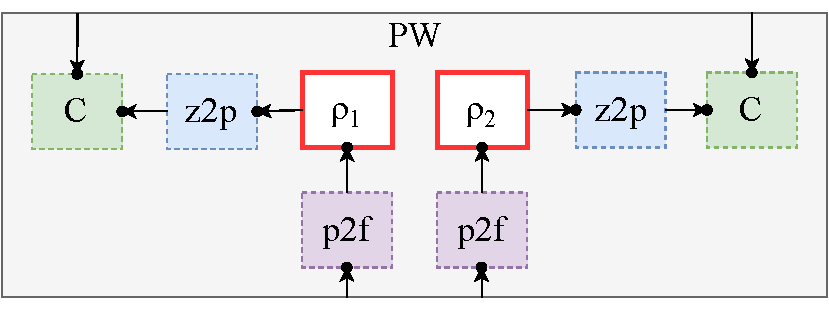
\includegraphics[scale=0.5]{figures/blankpartywrapper2.pdf}
\caption{The internals of the protocol wrapper with two parties. The arrows indicates the client/provider relationship between each pair: provider $\rightarrow$ client. The wrapper creates \texttt{z2p} to offer a channel and convert from gunctional to message type---the \texttt{p2f} do the same. A communicator is used because \texttt{z2p} cannot send message to real one with differing token type. The types of the processes offered are (color): \tgr{comm[z2pmsg[comp2f]]}, \tb{sender}, \tr{party[Int]}, \tp{comm[p2fmsg[rop2f]]}. }
%The processes \texttt{z2p} offer linear channels to their respective protocol parties that are typed according to that party's protocol, and they receive messages from virtual communicators that hold messages specific to one \texttt{pid}. The protocol code for $\pi_1$ and $\pi_2$ are user-specified and offer a channel to the \texttt{p2f} process according to their protocol with the functionality. The \texttt{p2f}s convert outgoing messages to, and incoming messages from, functional message types to be sent to/from the functionality. The protocol wrapper gives messages to the virtual communicators and receives messages from \texttt{p2f}s.}
\label{fig:blankpartywrapper}
\vspace{-1.5em}
\end{figure}

%For the commitment example, if $\pi_1$ and $\pi_2$ ran the commitment protocol, \inline{z2p} would offer a channel of type \inline{sender} and \inline{receiver} to $\pi_1$ and $\pi_2$, respectively, and it converts between the functional messages for the commitment protocol and the session typed ones. 
%In the ideal world, the $\pi_1$ and $\pi_2$ run a dummy protocol where their offered channels are simply forwarded to their \inline{z2p} channels, i.e. the \inline{z2p} and \inline{f2p} channels have the same type: \inline{sender} and \inline{receiver}, respectively.
%In the style of Nomos, the protocol wrapper:
%\begin{itemize}
%	\item Attempts to read messages incoming from \Z, \A, or \F and forward them to the appropriate process depending on \inline{pid}.
%	\item Read from the internal communicators or the \inline{p2f} processes for outcoing messages.
%\end{itemize}
%For reference the functional messages typed for the commitment protocol are:

%Recall the session types for the sender and receiver, with \Fcom, introduced in Section \ref{subsec:idealcommitment}.
%%\begin{gather}
%%	\mi{stype} \; \m{sender} = \ichoice{\mb{commit} : \m{bit} \product \m{scommitted}} \\
%%	\mi{stype} \; \m{scommitted} = \ichoice{\mb{open} : 1} \\
%%	\mi{stype} \; \m{receiver} = \echoice{\mb{commit} : \m{rcommitted}} \\
%%	\mi{stype} \; \m{rcommitted} = \echoice{\mb{open} : \m{bit} \arrow \one}
%%\end{gather}
%At the beginning there are no parties. When the \A or \Z write to a party with some pid $p$ the protocol wrapper creates $p$ if it does not exist.
%It creates and stores the session-typed channels or all of the parties in channels corresponding to their type and moves channels between them as the type evolves.
%For example for parties' channel with \Z the protocol wrapper generates the following lists:
%\begin{gather}
%	\m{R1L1}[\m{sender}] \\
%	\m{R1L2}[\m{scommitted}] \\
%	\m{R2L1}[\m{receiver}] \\
%	\m{R2L2}[\m{rcommitted}] 
%\end{gather}
%At the beginning of the protocol, the committer's \msf{z2p} channel would be in \inline{R1L1} and the receiver's is in \inline{R2L1}.
%The channel's connection the protocol wrapper to the rest are still functionally typed. It's channel \inline{p2f} will still be typed \inline{#ptof: comm[p2fmsg[comp2f]]} where \inline{comp2f} is:
%Succinctly, the protocol wrapper functions as follows:
%\begin{itemize}
%\item When the protocol wrapper receives a message for some \msf{pid}, if the party doesn't exist the protocol wrapper creates all the party's channel parameterized by the correct session types (the role of the party is determined by the incoming message). The channels are stored and outgoing channels are waiting to be read from.
%\item The message sent to the party with the session type is determined by the functional type. The wrapper creates a session-typed message and forwards the contents of the message to the party.
%Despite accepting functionally typed messages, the protocol wrapper uses session types in this way to allow the type checker to catch invalid and out of order environments, adversaries and functionalities. 
%For example, in the commitment protocol when the committer tries to commit a bit in \Fcom like this:
%\begin{lstlisting}[basicstyle=\small\BeraMonottFamily, frame=single, mathescape]
%$\$$p2f.commit 
%$\tb{send}$ $\$$p2f b
%$\tb{pay}$ {p2fn} $\$$p2f
%\end{lstlisting}
%\begin{lstlisting}[basicstyle=\small\BeraMonottFamily, frame=single, mathescape]
%$\$$p2f.SEND 
%$\tb{send}$ $\$$p2f pid 
%$\tb{send}$ $\$$p2f Commit(b)
%$\tb{pay}$ {p2fn} $\$$p2f
%\end{lstlisting}
%The party wrapper intercepts and converts it to a functionally typed message:
%\item For outgoing messages, the protocol wrapper does a similar conversion where it reads the sesion typed channel output by the party and converts its message to the appropriate functional message type.
%\end{itemize}

%\paragraph{Functionality Wrapper}
%The \fwrapper adopts a similar approach to the \partywrapper, except it only creates one instance of the underlying functionality.
%For the same reason as the \partywrapper, we use an \fwrapper to enable a dynamic set of parties.
%One caveat in supporting such functionalities, is that, so far, only functionalities whose type follows a specific form are allowed.
%In the random oracle type given below, notice that the type before and after a party interacts with it is the same: type $\m{party}[a]$.
%\begin{mathpar}
%\m{party}[a] = \textcolor{red}{\getpot^1} \ichoice{\mb{hash} : \m{pid} \arrow \m{int} \product \m{hashing}[a]} \\
%\m{hashing}[a] = \echoice{\mb{shash} : \m{pid} \arrow \m{int} \product \textcolor{red}{\paypot^0} \m{party}[a]} 
%\end{mathpar}
%A party queries a $\mb{hash}$ of an integer from \Fro and receives an integer as a response. The session type includes the \inline{pid}, which enables it to handle all parties over the same channel.
%
%An example of the internals of the \fwrapper are showing on the left-hand-side of Figure~\ref{fig:multisession}.
%Like the \inline{z2p} processes in the \partywrapper, \inline{S} and \inline{R} represent the sender and receiver in the commitment protocol, and they read from their virtual communicators and communicate with \Fcom over a session-typed channel.

%When a party invokes \Fro, the type it expects is \inline{party[a]}, and when it has received its hash the type is again back at \inline{party[a]}. 
%The wrapper handles such dynamic functionalities by channeling all party communication through one linear channel in the wrapper. 
%Therefore, \Fro reads on one channel and responds to the specific party with some \inline{pid}, and the protocol wrapper remains unchanged. 
%
%The constructions of the protocol wrapper and functionality wrapper enable users to write very simple ideal functionality and protocol code, as we will discuss in the next Section and in the Appedix.

%In the commitment example, \Fcom accepts two channels, one from each party, and two processes are created (call then \inline{p2f} for now) which offer channels of type \inline{sender} and \inline{receiver}, respectively. 
%The wrapper differs from the protocol wrapper for certain functionalities that accept a dynamic number of parties. 
%Continuing with our commitment example, the random oracle functionality, an idealized hash function, is used in the real world to realize \Fcom, and it allows a dynamic set of parties to inteact with it.
%Its session type with protocol parties is given below.
%The session type is special in that, for every interaction, the channels type always ends up back at \inline{party[a]} before any other party tries to use \Fro.
%NomosUC enables ideal functionalities whose types work like this by adding the \inline{pid} to the type, and having only one process in the functionality wrapper offering a channel of this type to \Fro.
%Unlike \Fcom where new communicator and \inline{p2f} process is created for each new party, messages from all parties pass through one such process.
%Additionally, moving the \inline{pid} into the session type means that the protocol wrapper can create arbitrarily many \inline{pid}s to communicate with \Fro.

\paragraph{The Adversary}
The adversary, much like the environment, is providing input to the protocol and functionalities.
As the UC framework is concerned with modular construction for protocols, and NomosUC with using session types to aid in suc construction, we do not give adversaries session types.
Therefore, they are not wrapper like protocols and functionalities, and communicate with all other processes directly through functional message types.

\subsection{Polynomial Bound}
The security of the UC framework relies on computational constraints on adversaries, and, generally, on what all ITMs can do.
It introduces the concept of import tokens as a new way to reason about ITMs being polynomial in the security parameter $k$. 
The import mechainsm as described in UC, and which we descrive in Section~\ref{sec:background}, ensures that a single ITM's execution is upper-bounded by some poynomial $T(n,k)$ where $T$ is a polynomial, $n$ is its net import token balance (received - sent), and $k$ is the security parameter.
Canetti et al. limit their discussion to parameterized systems where all machines do not do anything until they have received at least $k$ import.
We depart from this notion slightly and express ``interactive polynomial time'' by using a bounding polynomial in both import and $k$.
We do this for two reasons.
First, it remedies our exclusion of ``parameterized systems'' by easing the import requirements of cacnonical cryprograpic operations, such as a random oracle operation on $k$-bit strings that would otherwise require $k$ import. 
Second, we add $k$ to reflect a more natural notion of import and modularity in UC by allowing minimial import for constant-work one-shot processes like \Fcom which no longer need import just to handle $k$-bit strings.

In NomosUC, we build import into the type system to be able to reason about ITMs being locally polynomial time given some polynomial $T$.
Specifically, the system provides novel constructs to exchange import, generate potential from that import, and create virtual import for simulating other machines.
%Specifically, the type system can check whether a given polynomial bound in the import amount satisfies the potential generated/used by an open Nomos term.
The language additionally encodes the computational cost of each operation performed by an ITM, and statically guarantees that the execution cost of each ITM is locally polynomial in the net import it has over its entire execution. 
The locally polynomial invariant can be extended to claim that the entire UC execution of locally PPT ITMs is also PPT.

\begin{ddef}[PPT in $k$]\label{def:ppt}
A term $e(k,r)$ is \emph{well-resource-typed} and PPT if, given some amount of initial import $n$, there exists a polynomial $T(n,k)$ such that $\forall k, r, e(r,k) \{n\}$ terminates in at most $T(n,k)$ steps. 
\end{ddef}

%\begin{proof}
%The Nomos type system only type checks programs for which a satisfying assignment of polynomial $T$ is possible.
%Given an $n \in poly(k)$, all programs that type check must be \textit{well-resource-typed.}
%%The Nomos type system guarantees that a satisfying assignment of $n$ and $T$ will correctly type-check.
%%Therefore, given an initial amount of import $n(k) \in poly(k)$, the existence of some $T$ ensures that any process, regardless of its randomized execution according to the bit sequence $r$, $e$ is guarantees to be upper-bounded by $poly(k)$ satisfying the definition of probabilistic polynomial time in $k$.
%\end{proof}

%We demonstrate that our local PPT definition implies a PPT UC execution by adapting Proposition 7 from the UC framework to the NomosUC setting.
%Our sandboxing mechanism and \inline{withdrawTokens} procedure let us simulate the well-resource-typed ITMs, in the UC execution, within one ITM.
%We need only provide a suitable ``exchange rate function'' \GlobalF and a bounding polynomial $T$ on the single machine to conclude that it is well-resource-typed.
%If the initial import given to the system is $n$ then the single ITM generates $n$ virtual tokens, and simulates all inputs generated by the environment.
%Subsequently a sufficient bounding polynomial for this ITM is to the order of $O(n \times T')$ wher $T'$ is the largest polynomial among those bounding the simulated machines. The additional factor of $n$ exists to allow for routing/handling of messages between simulated machines.
%Clearly, this is not a tight bound but it will bound the entire UC execution, and our \inline{withdrawTokens} rules ensures that we are left with a valid token context.
%Therefore, the resulting UC execution, as a single ITM, is also well-resource-typed.

The soundness of our polytime notion comes down to showing that our UC experiment is PPT in only the security parameter $k$. 
The UC framework provides a simulation of a configuration of ITMs on a universal turing machine and proves that such a turing machine is also bounded by a polynomial $T$. 
Given the initial input of import tokens into the machine ($poly(k)$ amount of import), it can conclude that their import mechanism falls in line with the standard notion length-of-input polynomial time and satisfied their ``PPT in $k$'' definition. 
In NomosUC, we do not deal directly with ITMs, however, our type system allows us to judge whether a process, or collection of processes through the Preservation Theorem~\ref{thm:preservation}, is locally PPT given a particular polynomial. 
We use this judgement as a foundation and adapt Proposition 7 from UC~\cite{uc} to NomosUC, and show that our notion of locally PPT leads to a UC execution that is PPT in the security parameter $k$.

\todo{Define \F, \A, \Z, \m{PW}(\PI) as configurations that include the communicators to be used. Just need to create a standard for which direction communicator is part of which configuration.}
\begin{theorem} \label{thm:soundness}
Let \F, \A, \Z, and \m{PW}(\PI) be locally PPT configurations bounded by super additive polynomials $T_\F$, $T_\A$, $T_\Z$, $T_\PI$. Let \m{UC} be a configuration composed of a single process that runs \inline{execUC},. If \m{UC} receives $n \in poly(k)$ import initially, then the composed configuration $\m{UC} = \m{execUC} \; || \; \Z \; || \; \A \; || \; \m{PW}(\PI) \; || \; \F$ is PPT in $k$, where \m{PW} is the \partywrapper.
\end{theorem}

\begin{proof}
The resulting configuration \m{UC} has only one channel in it's context: the channel offered by \inline{execUC} of type \inline{Bit}. 
\inline{execUC}, therefore, is the intial process in the configuration and receives the intial import $n \in poly(k)$.

By the \m{compose} rule, the work done by the resulting configuration is strictly the sum of the work done by the composed configurations. 
The Preservation Theorem in conjunction with \m{compose} ensures type safety of \m{UC}, and allows us to concluce a sufficient bound on the total work done in \m{UC} by the polynomial $T'(n,k) = T_\A(n,k) + T_\Z(n,k) + T_\P(n,k) + T_\F(n,k) + O(1)$ where $n$ is the initial import into the system, and the addition $O(1)$ accounts for the constant bound on \inline{execUC}.
If we take the intial import $n$ to be polynomial in the security parameter $k$, we conclude that \m{UC} is PPT in $k$.
\end{proof}

\paragraph{Sending/Receiving Import}
Our construction of the UC experiment requires communicators (introduced in Section~\ref{sec:nomosuc}) to intermediate communication between the \Z, \A, \F, and \m{PW}(\PI).
Their use adds import requirements to the experiment that are not captures by just the types of \F, \A, and \PI. 
It results from them being activates a potentially polynomial number of times. Therefore, the communicator's type, introduced in Section~\ref{sec:nomosuc} defines the, reflects this computation by
retaining one of the import tokens that is sent accross it. 
Given that our functionalities are parameteric in the amount of import they send/receive (so as to not restriction wat protocols can realize them), the user must take into account the number of import taken by communicators.
In our commitment example, the messages from \Z that uses the most import in the real world is the sending the \inline{open} message to the committer. This activationa results in 5 communicators being activated and so five more import than the protocol already requires. As long as the ideal functionality is parameterized to accept the same amount of import, indistinguishability still holds. \todo{This belongs somewhere else}.

%Our construction of the \partywrapper and \fwrapper rely on sending functional messages between them through a shared communicator.
%The same holds true between the adversary and the two wrappers, and also holds true between the environment and the \partywrapper.
%When any of these parties is sending import to each other, they must always send the maximum import of any message that can be exchanged with each other.
%For example if parties $p_1$ and $p_2$ send $n_1$ and $n_2$ import to the functionality, then the communicator between the \partywrapper and \fwrapper will be typed to expect $max(n_1, n_2)+1$ import on every message from the \partywrapper and vice versa for messages from \fwrapper to \partywrapper. 
%Recall from Section~\ref{sec:nomosuc} that the $+1$ is required to give the communicator at least one unit of import.
%Similarly, \Z will send the maximum of the imports required by $p_1$ and $p_2$ plus two additional import for communicators.
%In total, for any activation by \A or \Z there can be up to three communicators activated in the execution. 

%An simple example where that illustrates the type system's capabilities is the authenticated append/read functionality $\F_\msf{AppRd}$~\footnote{We provide the code for this functionality in the appendix for the simplified case of a single party.}.
%The functionality requires parties to provide 1 unit of import to append items to the list and 1 unit of import to read from the list, and the functionality generates potential proportional to the length of the list in order to traverse it.
%It is clear that the total work performed by $\F_\msf{AppRd}$ is bounded by a quadratic poynomail, and the NomosUC type system ensures that only bounding polynomials quadratic or larger successfully type check.
%\todo{something more to say here}

%\begin{definition}[PPT Term]\label{def:pptterm}
%A \textit{PPT term} is a \textit{well-typed} term $e(k, r)$ that is \textit{closed} except for security parameter $k$, random bit sequence $r$.
%\end{definition}
%
%We first-define terms that are well-typed in the traditional session-types-sense in Definition~\ref{def:pptterm}, i.e. without any resource constraints~\cite{caires2010session}.
%Such terms are closed except for the security parameter $k$ and some uniformly random bit sequence $r$. 

%However, we also want to reason about terms that are well-typed when connected to another Nomos terms.

\subsection{Emulation}
Emulation underpins the UC security definition, and reasons about indistinguishability between two protocols over all adversaries against it and a simulator for all environments.
In NomosUC, we must be more careful to only consider protocols and adverasaries whose types (both message and import) match over the channels they share. 
Therefore, we introduce the term \textit{well-matched} to mean a PPT term $e$ is well-typed when connected to another term $e'$.
Simply put, we want to capture terms $e$ and $e'$ that can be connected over the channels the share given their type.
The resulting terms in Definition~\ref{def:wellmatched} are partionall closed after connection: the terms may only be connected on some subset of their channels.
%Simply put, the channels that $e$ and $e'$ share are of the same type. 
%Specifically, we want to exclude processes that logically share a channel, say the channel from \inline{p} to \inline{f}, but send (their types message types don't match).
%This new definition becomes important when we discuss UC emulation below as we want to reason about environments that are \textit{well-matched} for a protocol $\pi$ or a specific adversary \A.

\begin{ddef}[Well-Matched]\label{def:wellmatched}
\begin{mathpar}
\footnotesize
\inferrule*[right=Well-matched]
{\Tokens_1, K \semi \Delta_1 \vdash e :: \Delta_1' \semi 
\Tokens_2, K \semi \Delta_2 \vdash e' :: \Delta_2' \\ \\
 S \equiv \Delta_1 \bigcap \Delta_2 \neq \emptyset}
%{\Delta_1 \leftrightarrow \Delta_2}
{\Delta_1 \equiv_{S} \Delta_2 \semi e \leftrightarrow e'} 
\end{mathpar}
\end{ddef}

In the UC security definition, we say that a protocol $\pi$ posesses the same security properties as another protocol $\phi$ if no environment can distinguish between them for any adversary.
In most cases we compare a real protocol $\pi$ with an idealized protocol $(\idealP, \F)$ which is actually just an ideal functionality with dummy parties.
The ideal functionality is known to achieve the desired security processes because it acts like a simple, trusted third party.
%They are much simpler than protocols because they don't require any special code to handle mutually distrustful other processes, and they perform the given computation on behald of the ideal world parties.

Given the random choices ITMs in UC can make, it is clear that the outputs of \inline{execUC} produces and ensemble of distributions over all possible random bitstrings and security parameters.
Emulation, then, is about the ensembles created by two UC environments being computationally indistinguishable from each other.
We define indistinguishabiliy between ensembles in a standard way using \textit{statistical distance} in Definition~\ref{def:distance}.

\begin{definition}[Indisinguishability]\label{def:distance}
Two ensembles $\mathcal{D}_{1,k}, \mathcal{D}_{2,k}$ are indistinguishable, $\mathcal{D}_{1,k} \sim \mathcal{D}_{2,k}$, if their statistical distance is at most $negl(k), \forall k$.
\end{definition}

%\paragraph{Validity}
%For the remainder of this section we refer to \emph{valid} adversaries and simulators given a particular protocol, functionality, or environment.
%We refer to adversaries that type-check when connected to \Z, \F, or $\Pi$ by \inline{execUC}, and that are \emph{well-matched} as defined above. 
%Indisintiguishability between two protocols is defined as follows (we shorten the communicator type \msf{comm} to \msf{c}):

UC emulation combines the UC exeution with indistinguishability resuting in the following NomosUC emulation definition.
\begin{definition}[Emulation]\label{def:emulation}
Given two protocols $(\pi, \F_1), (\phi, \F_2)$ that are well-resource-typed then if $\forall \A$ well-matched with $(\pi, \F_1)$, $\exists \Sim$ s.t. $\forall \Z$ well-matched with \A and $(\pi, \F_1)$: \Sim is well-matched with $(\phi, \F_2)$, \Z is well-matched with $(\phi, \Sim)$, and $\msf{execUC}(\pi, \F_1, \Z, \A) \approx \msf{execUC}(\phi, \F_2, \Z, \Sim)$:

\begin{mathpar}
\footnotesize
	\inferrule*[right=emulate]
	{
		%. \models \msf{execUC}[\Tokentypes][\alpha] :: \Delta[\Tokentypes][\alpha] \\ \\ 
		% Protocols that are well-matched with their functionalities
		%\pi \rightarrow \Delta_1' \semi \phi \rightarrow \Delta_2' \semi \\
		\pi : \Delta_1'[\Tokentypes][\mathrm{T}_{\pi}] \semi \phi : \Delta_2'[\Tokentypes][\mathrm{T}_{\phi}] \semi \\
		%\langle \pi \leftrightarrow \F_2 \rangle, \langle \phi \leftrightarrow \F_1 \rangle \\
		% Type of execUC[DELTA_pi] and execUC[DELTA_phi]
		\forall \A \, | \, \Delta_4[\Tokentypes][\mathrm{T}_{\A}] \vdash \A :: \Delta_4', \langle \A \leftrightarrow \pi \rangle\\
		%\Delta_1'[\Tokentypes][\mathrm{T}_{\pi}] \equiv_{\Z} \Delta_1\ 
		%\semi \Delta_2'[\Tokentypes][\mathrm{T}_{\phi}] \equiv_\Z \Delta_2 \\
		% For all A if exists well-typed A that is well-matched with real world
		%\forall \A, (\exists (\Delta_4, \Delta_4') | \Delta_4 \vdash \A :: \Delta_4', \langle \A \leftrightarrow \pi \rangle, \langle \A \leftrightarrow \F_1 \rangle \\
		%\forall \A | \Delta_4 \vdash \A :: \Delta_4', \langle \A \leftrightarrow \pi \rangle, \langle \A \leftrightarrow \F_1 \rangle \\
		% implies simulator that is well-matched for ideal world
		%\Rightarrow \exists (\Delta_3,\Delta_3') \, | \, \Delta_3 \vdash \Sim_\A :: \Delta_3', \\ % \langle \Sim_\A \leftrightarrow \phi \rangle, \langle \Sim_\A \leftrightarrow \F_2 \rangle \\
		\Rightarrow \exists \Delta_3[\Tokentypes][\mathrm{T}_{\Sim}] \vdash \Sim_\A :: \Delta_3', \langle \Sim_\A \leftrightarrow \phi \rangle \\ % \langle \Sim_\A \leftrightarrow \phi \rangle, \langle \Sim_\A \leftrightarrow \F_2 \rangle \\
		% for all Z they that's well-matched for the real world => Z is well-matched with S and ideal world
		%\forall \Z (\langle \Z \leftrightarrow \A \rangle, \langle \Z \leftrightarrow \pi \rangle \Rightarrow \langle \Z \leftrightarrow \Sim_\A \rangle, \langle \Z \leftrightarrow \phi \rangle \\
		% and emulation has to hold
		\Rightarrow \forall \Z \; \msf{execUC} \ \pi\ \Z\ \F_1\ \A \approx\ \msf{execUC} \ \phi\ \Z\ \F_2\ \Sim_\A
	}
	{
		% EMULATION DEFINITION
		\lambda \A . \Sim_\A \vdash (\pi, \F_1) \sim (\phi, \F_2) % \F_1 \xrightarrow{\pi} \F_2
		%\lambda \A . \Sim_\A \vdash (\pi, \F_1) \sim (\phi, \F_2)
	}
\end{mathpar}
\end{definition}
The emulation definition above is quite straightforward. It starts with defining the protocols in question and their type under the type parameters passed to \inline{execUC}.
It then states that for all adversaries that are well-matched with $\pi$ and $\F_1$, there exists a simulator such that the two executions are indistinguishable. 
The definition ensures that for emulation to hold, the constructed simulator must be well-matched everywhere \A is well-matched: for all environments \A is well-matched with the \Sim must also be well-matched with.

With this emuluation definition we complete our definition of UC-realization in Definition~\ref{def:realize}.
If a simulator exists such that emulation holds for $(\pi, \F_1) \sim (\idealP, \F_2)$ then we say that the protocol $\pi$ UC-realied the functionality $\F_2$ in the $\F_1$-hybrid world:
\[
	\F_1 \xrightarrow{\pi} \F_2
\]

\paragraph{Import for Functionalities}
The \Fcom example use throughough this work is realized by protocol that uses the random oracle. 
A natural notion of import should define \Fcom as requiring 0 import because it is one-shot and halts after doing constant amount of work.
\Fro on the other hand, requires at least 1 unit of import in order to be handle a potentially polynomial mumber of activations as well as reading/writing $k$-bit strings.
This poses a problem that the ideal world requires 0 import however, the real world requires at least 1 unit of import.
We resolve this dilemma by defining functionalities as parameteric in the amount of import they require.
Parametric functionalities do not restrict UC-realization to only those protocols that are as compitatiaonally ``efficient'' as the them. In cryptography, it is common for real protocols to be computationally intensive while the ideal functionality they are realizing is trivial, and we want to be able to express such emulation.
We modify the arrow notation, slightly, to capture that a functionality can realize itself while requiring more import, and use the notation $\F^m$ to denote a functionality parameterized to require $m$ import.
\[
	\F_1^m \xrightarrow{\idealP} \F_2^{n \geq m}
\]
For the remainder of this work we do not bother import annotations on functionalities and only concern ourselves with the minimum import they require because it is an implementation detail.

%When we talk about emulation, we particularly care about emulation with respect to an ideal protocol $\phi$ which is really just $(\idealP, \F)$ where \idealP is the protocol which forwards all messages to/from \Z and \F.
%We say the protocol $\pi$ (potentially with a hybrid functionality $\F_1$) UC-realizes an ideal functionality $\F_2$ if Definition~\ref{def:emulation} holds for $(\pi, \F_1)$ and  $\phi = (\idealP, \F_2)$

%\begin{definition}[UC-Realize]
%A protocol $\pi$ UC-realized an ideal functionality $\F_1$ if $(\pi, \F_2) \sim (\idealP, \F_1)$ for some $\F_2$.
%
%\begin{mathpar}
%\footnotesize
%\inferrule*[right=UC-Realize]
%{ (\pi, \F_1) \sim (\idealP, \F_2) }
%{ \F_1 \xrightarrow{\pi} \F_2 }
%\end{mathpar}
%\end{definition}

\subsection{Dummy Lemma} \label{sec:dummy}
The dummy lemma is a crucial result in UC that reduces the design space of simulators to just one: for the dummy adversary in the real world.
The Lemma states that if a simulator exists for the dummy adversary, called the dummy simulator \DS, then there it is easy to construct a simulator for any other adversary \A. 
The simulator constructed in this lemma uses virtual tokens to internally run \DS and \A.

The intuitiom behind this results rests in the fact that emulation must hold over $\forall \Z$ for a particular \A. 
Particularly, in the case of \DS and \DummyAdv, emulation holds for a \Z that may be running any other possible \A internally and passing it's output to \DS and \DummyAdv.
Therefore, moving \A out of the simulation and into the execution, as the real adversary and as providing input to \DS, should maintain emulation between the two worlds.

\begin{theorem}[Dummy Lemma]\label{thm:dummy}
If \ $\exists \DS$ s.t. $ \DA, \DS \vdash \F_2 \xrightarrow{\pi} \F_1$ then $\forall \A \ \exists \Sim_\A$ s.t. $\Sim_{\A} \vdash  \F_2 \xrightarrow{\pi} \F_1)$ 
\end{theorem}

We give the proof of this lemma in the appendix, however, we provide an intuition for understanding why it is true.
Simulation w.r.t the dummy simulator works for all environments, even those that could run any potential real-world adverasry internally. Such environments, pass input to the adversary, whose output is given to the dummy simulator. 
The constructed simulator captures the idea of moving the adversary from the environment into the the execution, and the constructed simulator runs the real-world adverasry and dummy simulator internally.
Environment inputs are not passed to the adversary, and the adversary's outputs are passed to the dummy simulator.

%\begin{proof}
%The constructed simulator $\Sim_\A$ internally simulates \DS and \A through a virtual token type $K'$. 
%We describe the simulation pattern below to simulate messages to \DS and \A.
%
%On \inline{Z2A2P} input from \Z on channel \msf{z2a}, \Sim fowards the message to the internal \A with the same type but virtual tokens instead of real ones:
%\begin{lstlisting}[basicstyle=\small\BeraMonottFamily, frame=single,  mathescape, label={lst:sim}]
%msg = $\nrecv$ $\$$z2a ;
%$\nget$ $\$$z2a {z2an : K} ;
%$\tm{withdrawTokens}$ f K K1 z2an ;
%$\nsend$ $\$$a_z2a msg ;
%$\npay$ {z2an : K1} $\$$a_z2a ; 
%\end{lstlisting}
%
%Similarly, on \inline{A2P(pid,msg)} output from \A to a protocol party on channel \msf{a2p}, \Sim sends the message to \DS as input from \Z (type: \inline{Z2A2P(pid, msg)}:
%\begin{lstlisting}[basicstyle=\small\BeraMonottFamily, frame=single,  mathescape]
%pid = $\tb{recv}$ $\$$a_a2p ;
%msg = $\tb{recv}$ $\$$a_a2p ;
%$\tb{get}$ K1 $\$$aa2p {a2pn} ;
%$\tb{send}$ $\$$sd_z2a A2P(pid, msg) ;
%$\npay$ $\$$sd_z2a {z2an : K1} ;
%\end{lstlisting}
%
%$\Sim_\A$ accepts input from \Z and forwards it to the internal \A, which outputs to either the protocol parties or the ideal functionality. 
%\Sim forwards this output to \DS acting as input from the environment  and forward any outputs \DS creates to the intended recipients.
%Our main proof obligation here is to ensure that $\SIM{\A}$ in NomosUC is well-resource-typed for all well-resource-typed \A.
%The $\Sim_\A$ performs constant overhead on the simulattion of \A and \DS. Therefore, a sufficient bounding polynomial on the runtime of $\Sim_\A$ can be given as:
%\[
%T(n) = T_{\A,\DS}(n) + T_{\A,\DS}(n) + O(n)
%\]
%where $T_{\A,\DS}(n)$ is the greater of the two bounding polynomials for \DS and \A evaluated at $n$, and $n$ is the import that \Z sends to \A and \Sim. 
%We must also reason about the use of virtual tokens.
%Given that \A and \DS are well-resource-typed we can conclude that the virtual import tokens generated for activating \A and \DS never exceeds a polynomial in the number of real import tokens received by \Sim. 
%\end{proof}

\subsection{Single Composition}
In this section we present a composition operator for protocols that completes the single composition theorem, Theorem~\ref{thm:singlecomp}.
The composition operator allows replacement of a functioality with a protocol realizing it, and, potentially, any functionality that protocol uses.

Say a protocol $\pi$, using hybrid functionality $\F_1$, realizes functionality $\F_2$. 
For a protocol $\rho$ that uses $\F_2$, replacement results in parties of $\rho$ being directly connected to parties of $\pi$ within the \partywrapper.
The protocol party $\rho_i$ that is connected to its \inline{p2f} process with a channel of type $\mb{a}$ is connected to party $\pi_i$ with the same channel.
Party $\pi_i$ is, in turn, then connected to its \inline{p2f}.
This replacement is visually described in Figure~\ref{fig:replacement}.

%In this section we present a simplified composition theorem and a second theorem we call the squash theorem.
%These two theorems combine later in the section to prove the full UC composition theorem as it appears in the UC framework~\cite{uc}.
%
%Briefly the composition operator allows substitution of a functionality for a protocol that realized is. 
%The theorem states that a protocol that uses some functionaliy \F can replace with a protocol $\pi$ that realizes it along with any hybrid functionality $\pi$ uses.
%More specifically, in NomosUC, say a protocol $(\pi, \F_1)$ realizes some functionality $\F_2$.
%A protocol $\rho$ that uses $\F_2$ can replace is with instances of $\pi$ directly connected to the corresponding instances of $\rho$ \emph{within} the protocol wrapper, and the ideal functionality $\F_2$ being replaced by $\F_1$ in the functionality wrapper.

%We highlight first, that our protocol wrapper construction illustrated in \ref{fig:blankpartywrapper}, connects the internal process in that specific way to enable composition.
%Recal that the Nomos language has the concept of clients and providers for a give linear channel. Given to processes, the type of the channel changes depending on which process \emph{offers} the channel, i.e. is the provider, and who is the client.
%The arrows in Figure~\ref{fig:blankpartywrapper} illustrate the \emph{client} $\rightarrow$ \emph{provider} relationship.
%We illustrate how protocol replacement works in NomosUC in Figure~\ref{fig:replacement}.

\begin{figure}
\centering
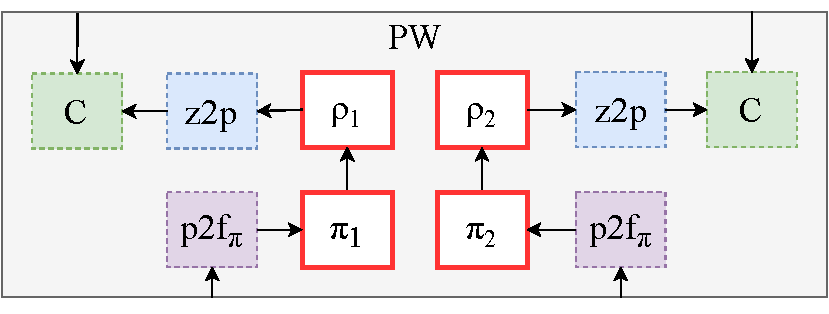
\includegraphics[scale=0.5]{figures/replacement2.pdf}
\caption{When we compose protocols we replace the \emph{p2f} process of $\rho$ with the corresponding instance of $\pi$ and its \emph{p2f} processes. By the emulation theorem, the channel offered by $\rho$ and accepted by $\pi$ have the same type.}
\label{fig:replacement}
\end{figure}

The code for the operator has the same type as any other protocol except, from the description above, it's offered channel is for the type of the functionality $\F_1$ instead of $\F_2$.
We rely on the code generation for to handle spawning instaces of a \inline{p2f} process corresponding to $\pi$ rather than $\rho$.
The operator is given in Figure~\ref{lst:compose}.
\begin{figure}
\begin{lstlisting}[basicstyle=\footnotesize\BeraMonottFamily, frame=single, mathescape]
$\tb{proc}$ compose[K][z,p]:
  (pid: Int), (rng: [Bit]), (sid: session[1]),
  (pid: Int), ($\$$z2p: z) |- ($\$$c: p) =
{
  $\$$ch <- PS.rho <- k rng sid pid $\$$z2p ;
  $\$$c <- Ps.pi <- k rng sid pid $\$$ch 
}
\end{lstlisting}
\caption{The composition operator accepts the same parameters as any other protocol party and offers the channel of type $p2f$ of the realizing protocol $\pi$. We connect $\rho$ to $\pi$ as an environment giving input to $\pi$. We do not need to include any import in our composition operator as the two protocols are guaranteed to be well-matched by the emulation definition. The operator replaces only one party (one \msf{pid}), and the \partywrapper instantiates parties that run the composed protocol.}
\label{lst:compose}
\end{figure}

The resulting composition operator, which composes the two simulators \SIM{\rho} and \SIM{\pi} inside the construction simulator, is best described in text as the resulting code is too verbose to include in the main body of this paper.
You can find the full simulator composition operator in the appendix.
\begin{itemize}
	\item Input from \Z is split between the two simulators
	\begin{itemize} 
		\item \inline{Z2A2P(pid, msg)} intended for parties of $\rho$ are passed to \SIM{\rho}
		\item \inline{Z2A2F(msg)} intended for $\F_1$ is passed to \SIM{\pi}.
	\end{itemize}
	\item Output from \SIM{\pi}: 
	\begin{itemize}
		\item \inline{A2F(msg)} for $\F_2$ and \inline{A2P(pid,msg)} for dummy parties of $\F_2$ are sent to \SIM{\rho} as \inline{Z2A2F(msg)}
		\item \inline{F2A2Z(msg)} is sent to \Z unaltered.
	\end{itemize}
	\item Output from \SIM{\rho}: 
	\begin{itemize}
		\item \inline{A2F(msg)} and \inline{A2P(pid,msg)} for $\F_3$ are sent out unaltered.
		\item \inline{F2A2Z(msg)} messages are sent to \SIM{\pi} as \inline{F2A(msg)} from $\F_2$.
		\item \inline{P2A2Z(pid,msg)} messages are sent to \Z unaltered.
	\end{itemize}
\end{itemize}
The simulator relies on simulators for $\F_1 \xrightarrow{\pi} \F_3$ and $\F_2 \xrightarrow{\rho} \F_3$ to satisfy simulation for Theorem~\ref{thm:singlecomp}.
It is clear that this construction adequately simulates the composed protocol. 
The type in the ideal world gurantees that both the real and ideal world adversaries get at least as much impor as any of the protocol parties. 
This ensures that the composed simulator has enough import to sandbox the two existing simulators and send import out to the ideal world parties and ideal funfctionality.
Therefore it is trivial to see that the composed simulator is well-resource-typed.

Another illustrative description of what composition proposes, logically, is shown by this series of UC executions where the $\equiv$ operator denotes equivalent UC executions that result from moving ITMs in and out of a sandbox, and $\approx$ indicates emulation:
\begin{align}
& \msf{execUC} \: \Z \, (\rho \circ \pi) \, \F_1 \, \DA \\
\equiv \; & \msf{execUC} \: (\Z \circ \rho) \, \pi \, \F_1 \, \DA \\
\approx \; & \msf{execUC} \: (\Z \circ \rho) \, \idealP \, \F_2 \, \SIM{\pi} \\
\equiv \; & \msf{execUC} \: \Z \, \rho \, \F_3 \, (\SIM{\pi} \circ \SIM{\rho})
%\approx \; & \msf{execUC} \: (\Z \circ \Sim{\pi}) \, \idealP \, \F_3 \, \Sim{\rho} \\
%\equiv \; & \msf{execUC} \: \Z \, \idealP \, \F_3 \, (\Sim{\pi} \circ \Sim{\rho}) 
\end{align}

%\item Inputs from \Z of \inline{Z2A2P(msg)} are passed to \SIM{\rho}, and inputs of \inline{Z2A2F(msg)} are passed to \SIM{\pi}.  
%\item \inline{P2A2Z(pid, msg)} outputs from \SIM{\rho} are forwarded to \Z unaltered.
%\item \inline{A2F(msg)} and \inline{A2P(pid, msg)} messages from \SIM{\pi} for $\F_2$ are sent to \SIM{\rho} as \inline{Z2A2F(msg)} and \inline{Z2A2P(pid, msg)}, respectively. 
%\item In the reverse direction, \inline{F2A2Z(msg)} messages from \SIM{\rho} are sent to \SIM{\pi} as \inline{F2A(msg)}, and, finally, \inline{F2A2Z(msg)} output generated by \SIM{\pi} is forwarded to \Z.
%\item \inline{A2P(pid,msg)}, \inline{A2F(msg)} messages from \SIM{\rho}, and \inline{P2A(pid,msg)} and \inline{F2A(msg)} from $\F_3$, are forwarded unaltered. 
%\end{itemize}

%We also provide a composition operator for simulators to construct a simulator for the composed protocol. We connect the simulatorsin the following way
%\begin{figure*}
%\begin{lstlisting}[basicstyle=\small\BeraMonottFamily, frame=single, mathescape]
%$\tb{proc}$ sim_compose[K][a2r,r2a][a2p,p2a][a2f,f2a]:
%  (k: Int), (rnd: [Bit]), (sid: session[1]),
%  (#z_to_a: comm[z2amsg[a2r][a2f]]), (#a_to_z: comm[a2zmsg[r2a,f2a]]),
%  (#a_to_p: comm[a2pmsg[a2r]]), (#p_to_a: comm[p2amsg[r2a]]), (#a_to_f: comm[a2fmsg[a2f]]), (#f_to_a: comm[f2amsg[f2a]])
%    |- ($\$$c: 1) =
%{
%  $\$$ch 
%\end{lstlisting}
%\end{figure*}

%\begin{figure*}
%\begin{lstlisting}[basicstyle=\small\BeraMonottFamily, frame=single,  mathescape]
%$\tb{proc}$ compose[K][z2r][r2z][f2r][r2f][p2f][f2p] : 
%    (pid: Int), ($\$$z_to_p: c[K][z2p]), ($\$$p_to_z: c[K][r2z]), 
%    ($\$$f_to_p: c[K][f2r]), ($\$$p_to_f: c[K][r2f])  |- ($\$$D : 1) =
%{
%	$\$$rho_to_pi <- $\tm{createchan}$[K][p2f];
%	$\$$pi_to_rho <- $\tm{createchan}$[K][f2p];
%
%	 <- pi  <-                 $\$$rho_to_pi $\$$pi_to_rho $\$$p_to_f $\$$f_to_p ;
%	 <- phi <- $\$$z_to_p $\$$p_to_z $\$$rho_to_pi $\$$pi_to_rho ; 
%}
%\end{lstlisting}
%\caption{Composition operator in Nomos that connects a protocol $\rho$ to a protocol $\pi$ that uses some functionality $\F$. The operators creates new channels to connect the realizing $\pi$ and it's hybrid \F. Output from $\rho$ intended for the replace functionality are actually send to parties of $\rho$, and channels outgoing from the parties to the functionality are given to $\pi$.}
%\label{lst:compose} 
%\end{figure*}

%\begin{theorem}[Composition]\label{thm:singlecomp}
%\begin{mathpar}
%\inferrule*[right=single-compose]
%{
%	\F_1 \xrightarrow{\pi} \F_2 \semi \F_2 \xrightarrow{\rho} \F_3 \\
%}
%{
%	\F_1 \xrightarrow{\rho \circ \pi} \F_3
%}
%\end{mathpar}
%
%If \textit{well-typed} $(\pi, \F_1$) realizes $\F_2$ and ($\rho$, $\F_2$) realizes some $\F_3$, then $(\rho \circ \pi, \F_2)$ is \textit{well-typed} and realizes $\F_3$ when $\circ$ is defined as in Figure~\ref{lst:compose}.
%\end{theorem}

%\begin{proof}
%The pre-condition ensures the existence of \textit{well-resource-typed} simulators $\Sim_\rho$ for $\F_2 \xrightarrow{\rho} \F_3$ and $\Sim_\pi$ for $\F_1 \xrightarrow{\pi} \F_2$, and, it is obvious that the composed protocol is also well-resource-typed.
%We construct a simulator \Sim' for the dummy adversary to show
%\[
%	\msf{execUC}\ (\rho \circ \pi)\ \F_1\ \Z\ \A \approx \msf{execUC}\ \idealP\ \F_3\ \Z\ \Sim''
%\]	
%
%The simulator $\Sim'$ relies only simulating \SIM{\pi} and \SIM{\rho}.
%Note that \SIM{\pi} can accept messages for $\pi$ or $\F_1$, simulate them, and generate input for $\F_2$. 
%Similarly, \SIM{\rho} can take inputs for $\rho$ or $\F_2$, simulate them, and generate input for $\F_3$.
%Therefore, we connect the two simulators in the natural way:
%\begin{itemize}
%\item Inputs from \Z of \inline{Z2A2P(msg)} are passed to \SIM{\rho}, and inputs of \inline{Z2A2F(msg)} are passed to \SIM{\pi}.  
%\item \inline{P2A2Z(pid, msg)} outputs from \SIM{\rho} are forwarded to \Z unaltered.
%\item \inline{A2F(msg)} and \inline{A2P(pid, msg)} messages from \SIM{\pi} for $\F_2$ are sent to \SIM{\rho} as \inline{Z2A2F(msg)} and \inline{Z2A2P(pid, msg)}, respectively. 
%\item In the reverse direction, \inline{F2A2Z(msg)} messages from \SIM{\rho} are sent to \SIM{\pi} as \inline{F2A(msg)}, and, finally, \inline{F2A2Z(msg)} output generated by \SIM{\pi} is forwarded to \Z.
%\item \inline{A2P(pid,msg)}, \inline{A2F(msg)} messages from \SIM{\rho}, and \inline{P2A(pid,msg)} and \inline{F2A(msg)} from $\F_3$, are forwarded unaltered. 
%\end{itemize}
%It is clear that \Sim' is able to emulate inputs from \Z to both parties of $\rho$ and the ideal functionalty $\F_1$.
%\Sim' performs constant over head in simulating two \emph{well-resource-typed}, and therefore it is clear that \Sim' is \emph{well-resource-typed}.
%When combined with the \emph{dummy lemma}, a well-resource-typed simulator exists for composition for any adverasry \A. 
%The dummy lemma presented above ensures that a simulator for any \A can be constructed that is well-resource-typed for all wel-resource-typed \A.
%\end{proof}
%
%We give a simpler, high-level idea of the forst step of the proof proof here which can be understood visually:
%The $\equiv$ operator is a result of moving around ITMs (some from within other ITMs into the main UC execution) and $\sim$ refers to indistinguishability.
%In line (13) above, $\rho$ is moved into the execution environment with an unchanged simulator as no additional simulation is required: the simulator allows unfettered communication between parties of $\rho$ and \Z.

\subsection{Multisession}

\begin{theorem}[Composition]\label{thm:composition}
\begin{mathpar}
\inferrule*[right=compose]
{
	%(\pi, !\F_1) \sim (\idealP, F_2) \semi (\rho, !\F_2) \sim (\idealP, \F_3) \\ 
	!\F_1 \xrightarrow{\pi} \F_2 \semi !\F_2 \xrightarrow{\rho} \F_3 \\
	%\Rightarrow \exists \Sim(\A) \vdash (\rho^{!\F_2 \rightarrow (!\pi \, \circ \, \msf{squash})}, !\F_1) \sim (\idealP, \F_3)
}
{
	!\F_1 \xrightarrow{\rho \, \circ !\pi \circ \, \msf{squash}} \F_3
	%(\rho \, \circ \, !\pi \circ \msf{squash}, !\F_1) \sim (\idealP, \F_3)
}
\end{mathpar}
\end{theorem}
Full composition in the UC framework extends beyond the simpler composition in Theorem~\ref{thm:singlecomp} which only defines replacement of one functionality with a protocol that realizes it.
Instead, UC composition allows for replacement of any number of instances of a functionality with instancesof the realizing protocol.
Theorem~\ref{thm:composition} illustrates the full composition theorem using our arrow notation, and highlights a theorem that we must prove before we can achieve full composition.
It relies on Theorem~\ref{thm:squash} that introduces the \msf{squash} protocol and the $!$ operator.
Notice that Theorem~\ref{thm:compose} follows directly from Theorem~\ref{thm:singlecomp} and Theorem~\ref{thm:squash}.

The multi-session extension of a protocol or functionality, specified by the $!$ operator (such as $!\rho$ or $!\F$), allows multiple instances of the protocol/functionality to be run within a sinlge ITM.
An ITM simulates the instances and multiplexes input/output to/from them much like the \partywrapper.

\begin{theorem}[Squash Theorem]\label{thm:squash}
%If a functionality \F is well-resource-typed, then $!\F$ and $!!\F$ are well-resource-typed (by Theorem~\ref{thm:bangppt}) and $(\idealP, !!\F) \sim (\msf{squash}, !\F)$.
%\textit{Well-resource-typed} \F $\Rightarrow$ $!\F \xrightarrow{\msf{squash}} !!\F$%  $(\idealP, !!\F) \sim (\msf{squash}, !\F)$
\begin{mathpar}
\inferrule*[right=squash]
{
\textit{well-resource-typed} \; \F
}
{
!\F \xrightarrow{\msf{squash}} !!\F
}
\end{mathpar}
\end{theorem}

For the multisession extension of a fuctionality, the type is straightforward and ony acts to multiplex input/outpt based on the intended target \inline{ssid}.
\begin{center}
\parbox{0cm}{
\begin{tabbing}
$\m{{P2MS}[a,b]\{n,m\}} = \textcolor{red}{\getpot^n} \ichoice{\mb{Inp}: ssid \arrow a \tensor \echoice{$\=$\mb{Ok}: \textcolor{red}{\paypot^0} \; \m{P2MS[a,b]\{n,m\}},$ \\
\>$\mb{Out}: ssid \arrow b \tensor \textcolor{red}{\paypot^m} \; \m{P2MS[a,b]\{m,n\}}}}$
%\m{MS2P[a][b]\{n,m\}}}$ \\
%\mi{stype} \; \m{{MS2P}[a][b]\{n,m\}} = \echoice{\mb{Ok}: \textcolor{red}{\paypot^0} \; \m{P2MS[a][b]\{n,m\}}, \mb{Out}: ssid \product b \arrow \textcolor{red}{\paypot^m} \; \m{P2MS[a][b]\{n,m\}}}  
\end{tabbing}}
\end{center}
The multisession extension is mentioned in greater detail in the appendix.
%and the functional types that are sent to the wrapper surrounding it are given by
%\begin{lstlisting}[basicstyle=\small\BeraMonottFamily, mathescape]
%$\yo{type}$ p2ms[a] = P2MS of ssid ^ a ;
%$\yo{type}$ ms2p[b] = MS2P of ssid ^ b ;
%\end{lstlisting}
%It is important to note that we require a session type here instead of allowing !\F act as the functionality wrapper because, when composed it must communicate directly communicate, over a session-typed channel, to another protocol.
%Furthermore, the construction of !\F is the same as in the \Fro example: one session typed channel for all parties.
%In Figure~\ref{fig:multisession} illustrated the functionality wrapper (right) and the multisession extension (left) for \Fcom. 
%\begin{figure}
%\centering
%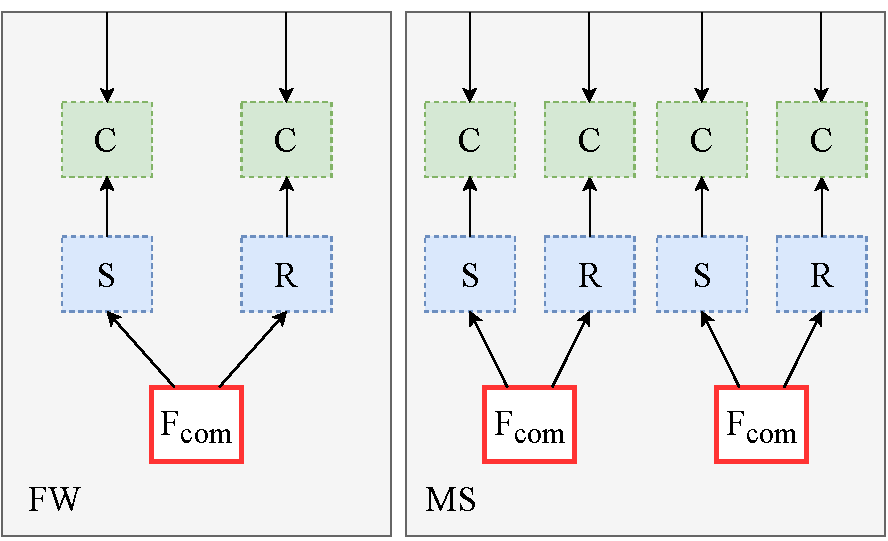
\includegraphics[scale=0.5]{figures/multisession.pdf}
%\caption{The multisession extension of \Fcom (right) with only two instances, creates the same processes $S$ and $R$ (offering the session typed channel to \Fcom) for every created instance. A communicator per session buffers messages for the $S$ and $R$ processes to consume and forward along their session-typed channel to \Fcom.}
%\label{fig:multisession}
%\end{figure}

%As a generic construction provided by NomosUC, the multisession operator requires some code generation but only to accept an arbitrary number of virtual token types if the underlying \F simulators other processes. 
%Furthermore, similar to the functionality wrapper, the multisession operator constructs the processes around \F in the same way and spawns them on-demand.
%The process definition for $!\F_\msf{com}$ is shown in Figure \ref{lst:bangf} accepting two token types: the real token type $K$ and the virtual token type $K_1$ for instances of $\F_\msf{com}$.
%
%\begin{figure}
%\begin{lstlisting}[basicstyle=\footnotesize\BeraMonottFamily, frame=single, mathescape]
%$\tb{proc}$ bangF[K,K1][p2f,...] :
%  (k: $\tgr{Int}$), (rng: [Bit]), (sid: session[a]), 
%  ($\$$p: P2MS[p2f][f2p]) |- ($\$$ch: 1) =
%\end{lstlisting}
%\caption{The type definition for the multisession operator for functionalities and the correspond message type and import parameters. The operator for protocol parties is identical in code but differens in that the parameters to the \texttt{P2MS} type are for \texttt{Z2P} interaction.}
%\label{lst:bangf}
%\end{figure}

\begin{theorem}[PPT !]\label{thm:bangppt}
If a functionality $\F$ is well-resource-typed, then it's multisession extension $!\F$ is well-resource-typed.
\end{theorem}

We examine this theorem in greater detail in the appendix. 
At a high-level it is obvious that such a construction, activated polynomially many times, is well-resource-typed as long as the underlying functionality/protocol is well-resource-typed.
%\begin{proof}
%A \textit{well-resource-typed} \F guarantees a polynomial $T_{\F}$ bounding its execution.
%In the worse-case, the multisession operator must spawn a new instance of $\F$ an every activation. 
%Let $N_{\F}$ denote the total number of instances (and, hence, number of activations) of $\F$ created by the operator.
%Note that $N_{\F}$ is polynomial in the security parameter $k$ for all well-typed environments, protocols, and adversary.
%Therefore, there always exists a bounding polynomial to bound a polynomial number of simulated instances of \F.
%The polynomial can be given as:
%$$ P_{!\F}(n) = N_{\F} P_{\F}(n) + \mathcal{O}(N_{\F}) $$
%where the $\mathcal{O}(N_{\F})$ is due to the overhead of maintaining and accessing the set of all instances.
%
%Similarly, \F being \textit{well-resource-typed} ensures a valid token context for all processes it may simulate. 
%Therefore, it is clear that there exists a global connecting poltnomial $f$ that ensures a valid token context for $!\F$.
%\end{proof}


%\begin{figure}
%\begin{lstlisting}[basicstyle=\small\BeraMonottFamily, mathescape, frame=single]
%$\yo{type}$ p2bFmsg[a] = P2bF of ssid ^ a ;
%$\yo{type}$ p2bbFmsg[a] = P2bbF of ssid ^ ssid ^ a ;
%$\tg{(* z2p : comm[z2pmsg[p2bbf[a]]] *)}$
%$\tg{(* p2f : comm[p2fmsg[P2bf[a]]] *)}$
%pid = recv $\$$z2p ;
%m = recv $\$$z2p ;
%case m (
%  P2bbF(ssid1, ssid2, m) =>
%    send $\$$p2f P2bF(ssid1 + ssid2, m) ;
%)
%\end{lstlisting}
%\caption{The \textit{squash protocol} accepts a message intended intended for $!!\F$ of type \inline{P2MS[p2ms[a]][ms2p[b]]}, i.e. of the form $(\msf{ssid}_1, (\msf{ssid}_1, msg))$.
%It ``flattens'' it into a single $\msf{ssid}_3 = \msf{ssid}_1 + \msf{ssid}_2$ that can be passed to $!\F$. The result is the same number of instances of \F but behind only a single $!$ operator.}
%\label{fig:squash}
%\end{figure}

\begin{proof} (Theorem~\ref{thm:squash})
On examination the \msf{squash} theorem does constant work per activation and concantenates two \inline{ssid}s into one for messages going to the functionality and does the inverse for messages incoming from the functionality.
We provide more detail for a proof of Theorem~\ref{thm:squash} in the Appendix, however, it is clear to see that the this theorem holds with a trivial simulator.
%First we describe the \msf{squash} protocol where $!!\F$ are nested $!$ operators.
%The protocol accepts messages intended for $!!\F$ of type \inline{P2MS[p2ms[a]][ms2p[b]]}, i.e. of the form $(\msf{ssid}_1, (\msf{ssid}_2, msg))$, and ``flattens'' them into a single message of type $\inline{P2MS[a][b]}$, i.e. of the form $(\msf{ssid}_3, msg)$.
%
%In $(\idealP, !!\F)$, \idealP~expects to receive messages of the form $(\msf{ssid}_1, (\msf{ssid}_2, m))$ where $\msf{ssid_2}$ is a sub-session of $\F$ (i.e. instance) inside some $!\F$ with sub-session id $\msf{ssid}_1$ inside of $!!\F$ (the message accesses functionality $\F[\msf{ssid}_1][\msf{ssid}_2]$).
%The \msf{squash} protocol flattens the indexing of instances of \F and combines session ids $\msf{ssid}_1$ and $\msf{ssid}_2$ into a single \msf{ssid}: $\msf{ssid}_3 := \msf{ssid}_1 \cdot \msf{ssid}_2$.
%If follows intuitively that the view for the environment remains the same. 
%
%We construct a simulator such that:
%\[
%\msf{execUC} \, \Z \, \idealP \, !!\F \, \SIM{\msf{squash}} \approx \msf{execUC} \, \Z \, \msf{squash} \, !\F \DA 
%\]
%The simulator is very simple. 
%Inputs to/from parties/\Z for a corrupt party is forwarded unmodified.
%Input intended for $!\F$ of the form $(\msf{ssid}_1 \cdot \msf{ssid}_2, msg)$ is sent as $(\msf{ssid}_1, (\msf{ssid}_2, msg))$ to $!!\F$. 
%Output from $!!\F$ is modified inversely and sent to \Z.
%
%The proposed simulator is trivially analyzed to be \textit{well-resource-typed}.
%It performs constant work per activation and does ``real'' simulation other than message modification to/from $!!\F$.
\end{proof}

\subsection{UC Composition}
Finally, we can conlude with full composition in Theorem~\ref{thm:compose}.
The proof follows directly from Theorems~\ref{thm:singlecomp} and \ref{thm:squash}.

\begin{proof}
By Theorem~\ref{thm:singlecomp} we can construct a simulator \SIM{1} for $!!\F_1 \xrightarrow{\rho \, \circ \, !\pi} \F_3$.
Theorem~\ref{thm:squash} then allows us to ``squash'' $!!\F_1$ and construct a simulator using \SIM{1} for $!\F_1 \xrightarrow{\rho \, \circ \, !\pi \, \circ \, \msf{squash}} \F_3$
\end{proof}

\subsection{Design Discussion}
One of the core research questions that this work aims to study session types applied to the UC framework. 
In this section, we discuss how resource-aware session types impact the design of functionalities in NomosUC as well as which are implementable.
We use the two-way authenticated channel functionality \Fauth to througout this discussion.

In plain session types, communication between two parties $P_s$ and $P_r$ occurs over a single duplex channel.
In UC the role of the adversary as a message scheduler in \Fauth, the most common network channel model, means a more complicated functionaty involving $P_s$, $P_r$, \F, and \A. 
The simplest, and most common approach, to \Fauth is the following communication pattern: a party $P_s$ sends a message to \Fauth, \Fauth sends the message to \A and waits for \A to say \inline{OK} before delivering the message to $P_r$.
Since both parties can send a message and receive a message, it is unclear which process, \Fauth or $P$, will be active along that channel at any given time.
Session types require this information to be statically known when two processes are communicating over a single channel--making this communication pattern unexpressable over a single channel.

There a few ways to overcome this constraint. 
In general, even though the UC framework places few restructions of communication patterns, most functionalities stick to a few.
\Fauth, for example, can take a few forms:
\begin{enumerate}
\item (presented above) Receiver and adverasry are activated directly: \Fauth waits for \A to tell it to deliver the message.
\item \Fauth ``polling'' approach: messages from $P_s$ are buffered for both \A and $P_r$. \A and $P_r$ must ask \Fauth for new messages. This is a more invonconvenient method, but can be useful for novel functionality designs that need a channel.
\item ``polling'' but receiver is activated: the message is stored in a buffer for \A, and \A's deliver message directly sends it to $P_r$.
\end{enumerate}
The simplest way to implement \Fauth in NomosUC is ``polling'' approach. As far as we know, we can systematically tranform any UC functionality into one that uses ``polling''. 
The consequences are that polling is inconvenient from a programming point of view because \Z needs to continuously activate parties to ask for new messages.
Hope is not lost though, because it turns out our type system can express functionalities in all three of the ways listed above. 
The first, and most natural, approach only requires splitting communicating between $P$ and \Fauth into two unidirectional channels
Such an extension to NomosUC trivially modifies the \partywrapper to handle two channels instead of one, and the types of the channels can be succintly expressed as: 
\begin{center}
\parbox{0cm}{
\begin{tabbing}
$\m{sending}[a] = \textcolor{red}{\getpot^n} \ichoice{\mb{sendmsg}: \m{a} \tensor \m{sendmsg}}$ \\
$\m{receive}[a] = \textcolor{red}{\getpot^m} \echoice{\mb{recv}: \m{a} \tensor \m{receive}}$ \\
$\m{adv}[a] = \echoice{\mb{leakmsg}: a \tensor \ichoice{ \mb{ok}: \m{leakmsg}}}$
\end{tabbing}}
\end{center}
The first to correspond to the channels for sending from $P$ to \Fauth and the second in the opposite direction. The third is the adversary's channel at \Fauth.

A notable part of our contruction is the machinery created around the protocol parties and functionality that intemediate their communication with communicators and functionally-typed messages.
Recall that such compromises are required in order to allow a \emph{dynamic} number of parties in UC.
The session type of the shared channel of a communicator only allows for a fixed amount of import to be sent over it with every messages. 
Protocols and functionalities that send different amounts of import depending on the message, say $i_1,...,i_n$, must now send $\m{max}(\{i_j\})$ import with every messages.
For existing UC definitions this appears to be an issue of ensuring a machine has \emph{enough} import, however, we can systematically map any UC import definition to one that works in NomosUC~\footnote{The problem can be reduced to ensuring enough ``latent'' import needed to compute, and, because we aren't concerned here with \emph{tight} computational bounds the problem is quite easy to solve. We discuss in greater detail in the appendix.}.



%\caption{The \msf{execUC} function used for the two-party commitment example used througout this paper. Recall, the \msf{execUC} is customized insofar as it takes in some number of virtual token types (here, $K_1$) to enable machines that simulate other machines. In the commitment example, there is no such simulation happening at the protocol or functionality level, therefore only the real token type $K_1$ is used here. The funtion spawns all the necessary ITMs in the UC execution: the environment, the protocol wrapper, the functionalty (wrapped), and the adversary. Each is parameterized with the security parameter $k$ and a random bit sequence $\msf{rng} \in \{0,1\}^{poly(k)}$.
%At the end, the environment is started and it returns a bit $b$ which is its guess for which world it is in. The full code can be found in the Appendix.}
%\label{lst:execuc}
%\end{figure*}

%We separate NomosUC into two modules: generic code and protocol-specific code. 
%Therefore, the \inline{execUC} refers to user specified code through the \inline{PS} module which defines \inline{PS.env} for \Z, \inline{PS.func} for the functionality, \inline{PS.prot} for the protocol, and \inline{PS.adv} for the adversary.
Communication between all of the major processes in the UC execution (\Z, \A, \partywrapper, and \fwrapper) is done through communicators introduced in Section~\ref{sec:nomosuc}.
Communicators are restricted to only sending functionally types messages in NomosUC, and we give generic types, below, to all such messages.
\todo{Is this important to even have here? seems a useless implementation detail.}
\begin{lstlisting}[basicstyle=\footnotesize\BeraMonottFamily, frame=single, mathescape]
$\Type$ p2zmsg[a] = P2Z of pid ^ a ;
$\Type$ p2fmsg[a] = P2F of pid ^ a ;
$\Type$ f2pmsg[a] = F2P of pid ^ a ;
\end{lstlisting}

\paragraph{The Environment}
The environment is the first machine that \inline{execUC} spawns and receives from it the session id and list of corrupted parties for this execution.
Its offered channel type \inline{EtoZ} specifies the interaction between \inline{execUC} and \Z:
\begin{lstlisting}[basicstyle=\footnotesize\BeraMonottFamily, mathescape, frame=single]
$\Type$ EtoZ[a] = +{init: a ^ list[pid] -> exec} 
$\Type$ exec = &{start : output_bit} ;
$\Type$ output_bit = +{bit: Bit -> 1} ;

$\tb{proc}$ PS.env[K][z2p,...]{p2zn,...} : 
  (k: $\tgr{int}$), (r: [Bit]), (#ztop: comm[z2pmsg[z2p]]{z2pn}), 
  (#ptoz: comm[p2zmsg[p2z]]{p2zn})...  |- ($\$$z : EtoZ) $\tg{(* <- offered channel *)}$
\end{lstlisting}
The environment also accepts communicators, as parameters, for communication with the protocol parties and the adversaries (in both directions), and offer a channel \inline{$\$$z} of type \inline{EtoZ}.
The type (above) states \Z provides an \emph{sid} of some user-defined type \inline{a} and a list of the \emph{pid}s of corrupted parties. 
Finally, \inline{execUC} instructs it to \inline{start} (\emph{external choice}) and return a bit $b$ as its guess for which world it is in.

%The \inline{\{z2pn\}}, for example, specifies the amount of import that must be sent by \Z with every message to a protocol party.
%The rest of the processes---the adversary, protocol wrapper, and functionality--are declared in the same way except the type parameters they expect are different: the protocol wrapper would of course accept type parameters for communication between it and \F, \A, and \Z.
%Finally the type of the offered channel \inline{$\$$z} is the same for all environments and communicates the \inline{sid} and set of corrupt parties chosen by \Z to \inline{execUC}.
%The \inline{sid} and corrupt list are parameters to the rest of the processes that \inline{execUC} spawns. 

%The communicators created by \inline{execUC} always use the same parametric types. 
%For example, for communication with the protocol, the types look like:
%\begin{lstlisting}[basicstyle=\small\BeraMonottFamily, frame=single, mathescape]
%$\Type$ p2zmsg[a] = P2Z of pid ^ a ;
%$\Type$ p2fmsg[a] = P2F of pid ^ a ;
%$\Type$ f2pmsg[a] = F2P of pid ^ a ;
%\end{lstlisting}
%Subsequently, the channel from \Z to the protocol wrapper will be typed as: \inline{comm[z2pmsg[z2p]]\{z2pn\}} where \inline{z2p} is a protocol-specific message type.
%The protocol \inline{PS.prot} is not spawned by \inline{execUC}. Instead the process spawns the protocol wrapper (described below) which spawns parties with that run the code \inline{PS.prot}.
%When in the ideal world, the protocol is given as the ideal protocol: one where the protocol wrapper converts the message from type \inline{z2pmsg[a]} to type \inline{p2fmsg[a]} but forwards the contents unaltered.
%The protocol wrapper and functionality wrapper manage spawning the instance(s) of the functionality and protocol parties.
%Similarly, an environment \msf{PS.env} and adversary \msf{PS.adv} must be defined as well.
%The message types exchanged between the processes are provided directly to \msf{execUC} as type parameters of the form \msf{p2f}, \msf{f2p}, and so on. 
%The first thing \inline{execUC} does is create the communicators and the corresponding channels for the main processes of the execution. 

%A consequence of using communicators is that in the UC setting they require at least 1 unit of import, beacuse they are activated a potentially polynomial number of times. 
%Therefore, all communicators in NomosUC receive some amount of import $n$ and send out only $n-1$. 
%The user-specified protocol, environment, functionality, and adverasary must account for this to ensure suffiient import is given to them.
%\begin{lstlisting}[basicstyle=\small\BeraMonottFamily, frame=single, mathescape]
%#ptoz <- communicator_init[K][p2zmsg[p2z]]
%           {p2zn+1} ;
%#ztop <- communicator_init[K][z2pmsg[z2p]]
%           {z2pn+1} ;
%...
%\end{lstlisting}
%This is strictly a design decision where user-defined protocols only specify import token requirements for the protocol not taking communicators into account. 
%The processes that they write, though, must conform to this standard and send an import token in addition to the amount they need.
%An alternate design would be that all import type parameters take the additional import token into account and communicators send one less than they receive.
%The drawback of the latter approach is that that when communicating with a process directly rather than through communicators (say, when simulating), you're sending one extra token for no reason.

%Next, the environment \msf{PS.env} is spawned, \inline{execUC} receives the \inline{sid} and corrupt list from \Z, and, finally, the remainder of the processes are spawned with these inputs. 
%Finally, the environment executes its own code when activated by \msf{\$z.start}, given the initial amoutn of import \inline{n}, and returns a bit through \inline{$\$$z.output_bit} which is its guess whether it's in the real or ideal world:
%\begin{lstlisting}[basicstyle=\small\BeraMonottFamily, frame=single, mathescape]
%$\$$z.start
%$\tb{pay}$ $\$$z {n}
%$\$$d <- $\$$z
%\end{lstlisting}

\subsection{The \partywrapper}
NomosUC departs slightly from the standard UC framework by using a \partywrapper to encapsulate all protocol parties and run them internally.
Rather than passing protocol party channels as parameters to \Z or \A (supporting a static set of parties), the \partywrapper provides a single endpoint for all messages to parties.
Similarly we adapt a \fwrapper to function like the \partywrapper but on functionalities. The main pupose of this wrapper and the \partywrapper is to intermediate communication between the session types the functionality uses and the functionally typed messages exchanges through communicators.

Like \iexecuc, we genrate the \partywrapper based on the protocol or functionality being executed. 
Converting between functional and session-typed messages is an easy task to automate and we push that onto code generation rather than requiring a user to produce it.
The extra processes generated within the \partywrapper are shown in Fiure~\ref{fig:blankpartywrapper}.
%In a nutshell, the wrapper accepts messages from a communicator, say from \Z, demultiplexes it, converts its type to one over a session-typed channel and conveys it to the necessary protocol party.

Following along with Figure~\ref{fig:blankpartywrapper}, the generated processes \inline{C} are use to de-multiplex messages based on the \inline{pid} of the receipient, and the \inline{z2p} and \inline{p2f} processes convert messages between the session typed channels and the functional messages that are received.
The arrow notation in Figure~\ref{fig:blankpartywrapper} indicates the $\m{prodiver} \leftarrow \m{client}$ relationship for each channel and provides their types.

We elaborate on the processes \inline{z2p}. For the commitment protocol the messages received by the \partywrapper are type as 
\begin{lstlisting}[basicstyle=\footnotesize\BeraMonottFamily, mathescape]
$\yo{type}$ comp2f = Commit of Bit | Open ;
$\yo{type}$ comf2p = Committed | Open of Bit ;
\end{lstlisting}
and the \inline{z2p} process intercepts them and communicates to the party over a channel typed with the \Fcom session types in Section~\ref{sec:nomosuc}.
For example when \Z gives the command to commit to a bit, \inline{z2p} does the following:
\begin{lstlisting}[basicstyle=\footnotesize\BeraMonottFamily, frame=single, mathescape]
case msg (
  Commit(b) =>
    $\$$z2p.commit ;
    $\tb{send}$ $\$$z2p b ;
    $\tb{pay}$ {z2pn} $\$$z2p ;
\end{lstlisting}
where \inline{$\$$z2p} is the session-typed channel to the committer.
The \inline{f2p} processes does the same for communication between the parties and the functionality.

Virtualizing the protoocl parties means that the wrapper and the parties it runs are, effectively, using the same import and potential.
We reason that the \partywrapper and protocol parties it runs will always have enough import by noticing that the \partywrapper does constant work on each activation.
Therefore, if protocol parties intend to hold on to import, there is always a suficient polynomial to allow both the wrapper and the party to perform potentially polynomial computation.
\todo{Reword this to make it crisper}.

%Folling along with Figure~\ref{fig:blankpartywrapper}, the generatd processes \inline{z2p} and \inline{f2p} communicate with the party over a session-typed channel and perform the message type conversion mentioned above based on a simple message type mapping provided by the user.
%The \inline{z2p} process offers a linear channel to the party with the correct session type with \Z. 
%The wrapper reads messages from \Z, demultiplexes them based on \inline{pid} and puts them in the appropriate virtual communcator (the green box labeled \inline{C}) for the \inline{z2p} processes to read from, convert, and send to the party.
%The protocol party offers a linear channel of its type with \F, and \inline{p2f} converts this to a functional type. \inline{p2f} offers the same type as a communciator to the wrapper which reads the message and sends it to \F. 
%Figure~\ref{fig:blankpartywrapper} indicates the type of the offered channel for all the relevant processes within the wrapper. 

%In order to use session types, the each protocol party is internally connected to two processes \inline{z2p} and \inline{f2p} over with session-typed channels for their communication with \Z and \F, respectively.
%\inline{z2p} is connected to party-specific virtual communicators so that \inline{z2p} and \inline{f2p} can read/send messages from. It can not read/write directly to/from the actual communicators connecting the protocol wrapper because, being simulations inside the protocol wrapper, they do not use the same token type.
%In the case of the ideal world with \Fcom, the both of the sender's ($\pi_1$) channel with \inline{z2p} channels with \inline{z2p} and \inline{f2p} are typed as \inline{sender}, and the protocol party itself ($\pi_1$) just fowards messages from one channel to the other.

%The processes \inline{Z2p} and \inline{f2p} are generated for each party based on their session-type, and they convert between them and functional messages for incoming/outgoing communcation with \Z, \F, or \A. 
%For example in the commitment example, where the functional message type is given by: 
%\begin{lstlisting}[basicstyle=\footnotesize\BeraMonottFamily, mathescape]
%$\yo{type}$ comp2f = Commit of Bit | Open ;
%$\yo{type}$ comf2p = Committed | Open of Bit ;
%\end{lstlisting}
%the \inline{z2p} process does something like this for the sender (where \inline{msg} is received from its virtual communicator):
%\begin{lstlisting}[basicstyle=\footnotesize\BeraMonottFamily, frame=single, mathescape]
%case msg (
%  Commit(b) =>
%    $\$$z2p.commit ;
%    $\tb{send}$ $\$$z2p b ;
%    $\tb{pay}$ {z2pn} $\$$z2p ;
%\end{lstlisting}
%It sends a commit message over the linear channel with the sender, and pays the necessary amount of (virtual) import tokens with the message.
%When \Z, \A, or \F send a message to a party that doesn't exist, the \partywrapper creates the new party's \inline{z2p}/\inline{f2p} processes and an instance of the party itself, and it connects them together in the same way shown. 
%We do something similar for functionalities, in Appefix~\ref{app:fwrapper}

\begin{figure}
\centering
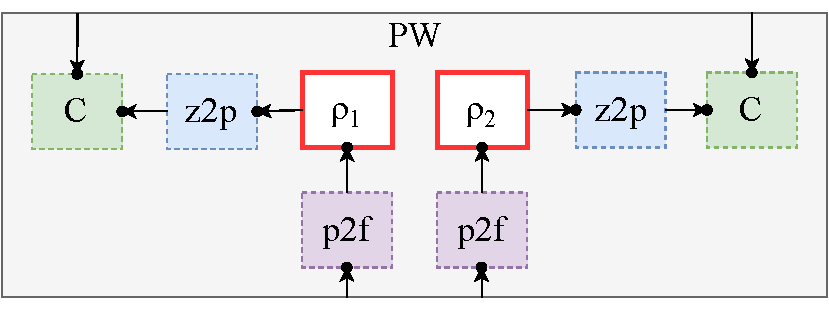
\includegraphics[scale=0.5]{figures/blankpartywrapper2.pdf}
\caption{The internals of the protocol wrapper with two parties. The arrows indicates the client/provider relationship between each pair: provider $\rightarrow$ client. The wrapper creates \texttt{z2p} to offer a channel and convert from gunctional to message type---the \texttt{p2f} do the same. A communicator is used because \texttt{z2p} cannot send message to real one with differing token type. The types of the processes offered are (color): \tgr{comm[z2pmsg[comp2f]]}, \tb{sender}, \tr{party[Int]}, \tp{comm[p2fmsg[rop2f]]}. }
%The processes \texttt{z2p} offer linear channels to their respective protocol parties that are typed according to that party's protocol, and they receive messages from virtual communicators that hold messages specific to one \texttt{pid}. The protocol code for $\pi_1$ and $\pi_2$ are user-specified and offer a channel to the \texttt{p2f} process according to their protocol with the functionality. The \texttt{p2f}s convert outgoing messages to, and incoming messages from, functional message types to be sent to/from the functionality. The protocol wrapper gives messages to the virtual communicators and receives messages from \texttt{p2f}s.}
\label{fig:blankpartywrapper}
\vspace{-1.5em}
\end{figure}

%For the commitment example, if $\pi_1$ and $\pi_2$ ran the commitment protocol, \inline{z2p} would offer a channel of type \inline{sender} and \inline{receiver} to $\pi_1$ and $\pi_2$, respectively, and it converts between the functional messages for the commitment protocol and the session typed ones. 
%In the ideal world, the $\pi_1$ and $\pi_2$ run a dummy protocol where their offered channels are simply forwarded to their \inline{z2p} channels, i.e. the \inline{z2p} and \inline{f2p} channels have the same type: \inline{sender} and \inline{receiver}, respectively.
%In the style of Nomos, the protocol wrapper:
%\begin{itemize}
%	\item Attempts to read messages incoming from \Z, \A, or \F and forward them to the appropriate process depending on \inline{pid}.
%	\item Read from the internal communicators or the \inline{p2f} processes for outcoing messages.
%\end{itemize}
%For reference the functional messages typed for the commitment protocol are:

%Recall the session types for the sender and receiver, with \Fcom, introduced in Section \ref{subsec:idealcommitment}.
%%\begin{gather}
%%	\mi{stype} \; \m{sender} = \ichoice{\mb{commit} : \m{bit} \product \m{scommitted}} \\
%%	\mi{stype} \; \m{scommitted} = \ichoice{\mb{open} : 1} \\
%%	\mi{stype} \; \m{receiver} = \echoice{\mb{commit} : \m{rcommitted}} \\
%%	\mi{stype} \; \m{rcommitted} = \echoice{\mb{open} : \m{bit} \arrow \one}
%%\end{gather}
%At the beginning there are no parties. When the \A or \Z write to a party with some pid $p$ the protocol wrapper creates $p$ if it does not exist.
%It creates and stores the session-typed channels or all of the parties in channels corresponding to their type and moves channels between them as the type evolves.
%For example for parties' channel with \Z the protocol wrapper generates the following lists:
%\begin{gather}
%	\m{R1L1}[\m{sender}] \\
%	\m{R1L2}[\m{scommitted}] \\
%	\m{R2L1}[\m{receiver}] \\
%	\m{R2L2}[\m{rcommitted}] 
%\end{gather}
%At the beginning of the protocol, the committer's \msf{z2p} channel would be in \inline{R1L1} and the receiver's is in \inline{R2L1}.
%The channel's connection the protocol wrapper to the rest are still functionally typed. It's channel \inline{p2f} will still be typed \inline{#ptof: comm[p2fmsg[comp2f]]} where \inline{comp2f} is:
%Succinctly, the protocol wrapper functions as follows:
%\begin{itemize}
%\item When the protocol wrapper receives a message for some \msf{pid}, if the party doesn't exist the protocol wrapper creates all the party's channel parameterized by the correct session types (the role of the party is determined by the incoming message). The channels are stored and outgoing channels are waiting to be read from.
%\item The message sent to the party with the session type is determined by the functional type. The wrapper creates a session-typed message and forwards the contents of the message to the party.
%Despite accepting functionally typed messages, the protocol wrapper uses session types in this way to allow the type checker to catch invalid and out of order environments, adversaries and functionalities. 
%For example, in the commitment protocol when the committer tries to commit a bit in \Fcom like this:
%\begin{lstlisting}[basicstyle=\small\BeraMonottFamily, frame=single, mathescape]
%$\$$p2f.commit 
%$\tb{send}$ $\$$p2f b
%$\tb{pay}$ {p2fn} $\$$p2f
%\end{lstlisting}
%\begin{lstlisting}[basicstyle=\small\BeraMonottFamily, frame=single, mathescape]
%$\$$p2f.SEND 
%$\tb{send}$ $\$$p2f pid 
%$\tb{send}$ $\$$p2f Commit(b)
%$\tb{pay}$ {p2fn} $\$$p2f
%\end{lstlisting}
%The party wrapper intercepts and converts it to a functionally typed message:
%\item For outgoing messages, the protocol wrapper does a similar conversion where it reads the sesion typed channel output by the party and converts its message to the appropriate functional message type.
%\end{itemize}

%\paragraph{Functionality Wrapper}
%The \fwrapper adopts a similar approach to the \partywrapper, except it only creates one instance of the underlying functionality.
%For the same reason as the \partywrapper, we use an \fwrapper to enable a dynamic set of parties.
%One caveat in supporting such functionalities, is that, so far, only functionalities whose type follows a specific form are allowed.
%In the random oracle type given below, notice that the type before and after a party interacts with it is the same: type $\m{party}[a]$.
%\begin{mathpar}
%\m{party}[a] = \textcolor{red}{\getpot^1} \ichoice{\mb{hash} : \m{pid} \arrow \m{int} \product \m{hashing}[a]} \\
%\m{hashing}[a] = \echoice{\mb{shash} : \m{pid} \arrow \m{int} \product \textcolor{red}{\paypot^0} \m{party}[a]} 
%\end{mathpar}
%A party queries a $\mb{hash}$ of an integer from \Fro and receives an integer as a response. The session type includes the \inline{pid}, which enables it to handle all parties over the same channel.
%
%An example of the internals of the \fwrapper are showing on the left-hand-side of Figure~\ref{fig:multisession}.
%Like the \inline{z2p} processes in the \partywrapper, \inline{S} and \inline{R} represent the sender and receiver in the commitment protocol, and they read from their virtual communicators and communicate with \Fcom over a session-typed channel.

%When a party invokes \Fro, the type it expects is \inline{party[a]}, and when it has received its hash the type is again back at \inline{party[a]}. 
%The wrapper handles such dynamic functionalities by channeling all party communication through one linear channel in the wrapper. 
%Therefore, \Fro reads on one channel and responds to the specific party with some \inline{pid}, and the protocol wrapper remains unchanged. 
%
%The constructions of the protocol wrapper and functionality wrapper enable users to write very simple ideal functionality and protocol code, as we will discuss in the next Section and in the Appedix.

%In the commitment example, \Fcom accepts two channels, one from each party, and two processes are created (call then \inline{p2f} for now) which offer channels of type \inline{sender} and \inline{receiver}, respectively. 
%The wrapper differs from the protocol wrapper for certain functionalities that accept a dynamic number of parties. 
%Continuing with our commitment example, the random oracle functionality, an idealized hash function, is used in the real world to realize \Fcom, and it allows a dynamic set of parties to inteact with it.
%Its session type with protocol parties is given below.
%The session type is special in that, for every interaction, the channels type always ends up back at \inline{party[a]} before any other party tries to use \Fro.
%NomosUC enables ideal functionalities whose types work like this by adding the \inline{pid} to the type, and having only one process in the functionality wrapper offering a channel of this type to \Fro.
%Unlike \Fcom where new communicator and \inline{p2f} process is created for each new party, messages from all parties pass through one such process.
%Additionally, moving the \inline{pid} into the session type means that the protocol wrapper can create arbitrarily many \inline{pid}s to communicate with \Fro.

\paragraph{The Adversary}
The adversary, much like the environment, is providing input to the protocol and functionalities.
As the UC framework is concerned with modular construction for protocols, and NomosUC with using session types to aid in suc construction, we do not give adversaries session types.
Therefore, they are not wrapper like protocols and functionalities, and communicate with all other processes directly through functional message types.

\subsection{Polynomial Bound}
The security of the UC framework relies on computational constraints on adversaries, and, generally, on what all ITMs can do.
It introduces the concept of import tokens as a new way to reason about ITMs being polynomial in the security parameter $k$. 
The import mechainsm as described in UC, and which we descrive in Section~\ref{sec:background}, ensures that a single ITM's execution is upper-bounded by some poynomial $T(n,k)$ where $T$ is a polynomial, $n$ is its net import token balance (received - sent), and $k$ is the security parameter.
Canetti et al. limit their discussion to parameterized systems where all machines do not do anything until they have received at least $k$ import.
We depart from this notion slightly and express ``interactive polynomial time'' by using a bounding polynomial in both import and $k$.
We do this for two reasons.
First, it remedies our exclusion of ``parameterized systems'' by easing the import requirements of cacnonical cryprograpic operations, such as a random oracle operation on $k$-bit strings that would otherwise require $k$ import. 
Second, we add $k$ to reflect a more natural notion of import and modularity in UC by allowing minimial import for constant-work one-shot processes like \Fcom which no longer need import just to handle $k$-bit strings.

In NomosUC, we build import into the type system to be able to reason about ITMs being locally polynomial time given some polynomial $T$.
Specifically, the system provides novel constructs to exchange import, generate potential from that import, and create virtual import for simulating other machines.
%Specifically, the type system can check whether a given polynomial bound in the import amount satisfies the potential generated/used by an open Nomos term.
The language additionally encodes the computational cost of each operation performed by an ITM, and statically guarantees that the execution cost of each ITM is locally polynomial in the net import it has over its entire execution. 
The locally polynomial invariant can be extended to claim that the entire UC execution of locally PPT ITMs is also PPT.

\begin{ddef}[PPT in $k$]\label{def:ppt}
A term $e(k,r)$ is \emph{well-resource-typed} and PPT if, given some amount of initial import $n$, there exists a polynomial $T(n,k)$ such that $\forall k, r, e(r,k) \{n\}$ terminates in at most $T(n,k)$ steps. 
\end{ddef}

%\begin{proof}
%The Nomos type system only type checks programs for which a satisfying assignment of polynomial $T$ is possible.
%Given an $n \in poly(k)$, all programs that type check must be \textit{well-resource-typed.}
%%The Nomos type system guarantees that a satisfying assignment of $n$ and $T$ will correctly type-check.
%%Therefore, given an initial amount of import $n(k) \in poly(k)$, the existence of some $T$ ensures that any process, regardless of its randomized execution according to the bit sequence $r$, $e$ is guarantees to be upper-bounded by $poly(k)$ satisfying the definition of probabilistic polynomial time in $k$.
%\end{proof}

%We demonstrate that our local PPT definition implies a PPT UC execution by adapting Proposition 7 from the UC framework to the NomosUC setting.
%Our sandboxing mechanism and \inline{withdrawTokens} procedure let us simulate the well-resource-typed ITMs, in the UC execution, within one ITM.
%We need only provide a suitable ``exchange rate function'' \GlobalF and a bounding polynomial $T$ on the single machine to conclude that it is well-resource-typed.
%If the initial import given to the system is $n$ then the single ITM generates $n$ virtual tokens, and simulates all inputs generated by the environment.
%Subsequently a sufficient bounding polynomial for this ITM is to the order of $O(n \times T')$ wher $T'$ is the largest polynomial among those bounding the simulated machines. The additional factor of $n$ exists to allow for routing/handling of messages between simulated machines.
%Clearly, this is not a tight bound but it will bound the entire UC execution, and our \inline{withdrawTokens} rules ensures that we are left with a valid token context.
%Therefore, the resulting UC execution, as a single ITM, is also well-resource-typed.

The soundness of our polytime notion comes down to showing that our UC experiment is PPT in only the security parameter $k$. 
The UC framework provides a simulation of a configuration of ITMs on a universal turing machine and proves that such a turing machine is also bounded by a polynomial $T$. 
Given the initial input of import tokens into the machine ($poly(k)$ amount of import), it can conclude that their import mechanism falls in line with the standard notion length-of-input polynomial time and satisfied their ``PPT in $k$'' definition. 
In NomosUC, we do not deal directly with ITMs, however, our type system allows us to judge whether a process, or collection of processes through the Preservation Theorem~\ref{thm:preservation}, is locally PPT given a particular polynomial. 
We use this judgement as a foundation and adapt Proposition 7 from UC~\cite{uc} to NomosUC, and show that our notion of locally PPT leads to a UC execution that is PPT in the security parameter $k$.

\todo{Define \F, \A, \Z, \m{PW}(\PI) as configurations that include the communicators to be used. Just need to create a standard for which direction communicator is part of which configuration.}
\begin{theorem} \label{thm:soundness}
Let \F, \A, \Z, and \m{PW}(\PI) be locally PPT configurations bounded by super additive polynomials $T_\F$, $T_\A$, $T_\Z$, $T_\PI$. Let \m{UC} be a configuration composed of a single process that runs \inline{execUC},. If \m{UC} receives $n \in poly(k)$ import initially, then the composed configuration $\m{UC} = \m{execUC} \; || \; \Z \; || \; \A \; || \; \m{PW}(\PI) \; || \; \F$ is PPT in $k$, where \m{PW} is the \partywrapper.
\end{theorem}

\begin{proof}
The resulting configuration \m{UC} has only one channel in it's context: the channel offered by \inline{execUC} of type \inline{Bit}. 
\inline{execUC}, therefore, is the intial process in the configuration and receives the intial import $n \in poly(k)$.

By the \m{compose} rule, the work done by the resulting configuration is strictly the sum of the work done by the composed configurations. 
The Preservation Theorem in conjunction with \m{compose} ensures type safety of \m{UC}, and allows us to concluce a sufficient bound on the total work done in \m{UC} by the polynomial $T'(n,k) = T_\A(n,k) + T_\Z(n,k) + T_\P(n,k) + T_\F(n,k) + O(1)$ where $n$ is the initial import into the system, and the addition $O(1)$ accounts for the constant bound on \inline{execUC}.
If we take the intial import $n$ to be polynomial in the security parameter $k$, we conclude that \m{UC} is PPT in $k$.
\end{proof}

\paragraph{Sending/Receiving Import}
Our construction of the UC experiment requires communicators (introduced in Section~\ref{sec:nomosuc}) to intermediate communication between the \Z, \A, \F, and \m{PW}(\PI).
Their use adds import requirements to the experiment that are not captures by just the types of \F, \A, and \PI. 
It results from them being activates a potentially polynomial number of times. Therefore, the communicator's type, introduced in Section~\ref{sec:nomosuc} defines the, reflects this computation by
retaining one of the import tokens that is sent accross it. 
Given that our functionalities are parameteric in the amount of import they send/receive (so as to not restriction wat protocols can realize them), the user must take into account the number of import taken by communicators.
In our commitment example, the messages from \Z that uses the most import in the real world is the sending the \inline{open} message to the committer. This activationa results in 5 communicators being activated and so five more import than the protocol already requires. As long as the ideal functionality is parameterized to accept the same amount of import, indistinguishability still holds. \todo{This belongs somewhere else}.

%Our construction of the \partywrapper and \fwrapper rely on sending functional messages between them through a shared communicator.
%The same holds true between the adversary and the two wrappers, and also holds true between the environment and the \partywrapper.
%When any of these parties is sending import to each other, they must always send the maximum import of any message that can be exchanged with each other.
%For example if parties $p_1$ and $p_2$ send $n_1$ and $n_2$ import to the functionality, then the communicator between the \partywrapper and \fwrapper will be typed to expect $max(n_1, n_2)+1$ import on every message from the \partywrapper and vice versa for messages from \fwrapper to \partywrapper. 
%Recall from Section~\ref{sec:nomosuc} that the $+1$ is required to give the communicator at least one unit of import.
%Similarly, \Z will send the maximum of the imports required by $p_1$ and $p_2$ plus two additional import for communicators.
%In total, for any activation by \A or \Z there can be up to three communicators activated in the execution. 

%An simple example where that illustrates the type system's capabilities is the authenticated append/read functionality $\F_\msf{AppRd}$~\footnote{We provide the code for this functionality in the appendix for the simplified case of a single party.}.
%The functionality requires parties to provide 1 unit of import to append items to the list and 1 unit of import to read from the list, and the functionality generates potential proportional to the length of the list in order to traverse it.
%It is clear that the total work performed by $\F_\msf{AppRd}$ is bounded by a quadratic poynomail, and the NomosUC type system ensures that only bounding polynomials quadratic or larger successfully type check.
%\todo{something more to say here}

%\begin{definition}[PPT Term]\label{def:pptterm}
%A \textit{PPT term} is a \textit{well-typed} term $e(k, r)$ that is \textit{closed} except for security parameter $k$, random bit sequence $r$.
%\end{definition}
%
%We first-define terms that are well-typed in the traditional session-types-sense in Definition~\ref{def:pptterm}, i.e. without any resource constraints~\cite{caires2010session}.
%Such terms are closed except for the security parameter $k$ and some uniformly random bit sequence $r$. 

%However, we also want to reason about terms that are well-typed when connected to another Nomos terms.

\subsection{Emulation}
Emulation underpins the UC security definition, and reasons about indistinguishability between two protocols over all adversaries against it and a simulator for all environments.
In NomosUC, we must be more careful to only consider protocols and adverasaries whose types (both message and import) match over the channels they share. 
Therefore, we introduce the term \textit{well-matched} to mean a PPT term $e$ is well-typed when connected to another term $e'$.
Simply put, we want to capture terms $e$ and $e'$ that can be connected over the channels the share given their type.
The resulting terms in Definition~\ref{def:wellmatched} are partionall closed after connection: the terms may only be connected on some subset of their channels.
%Simply put, the channels that $e$ and $e'$ share are of the same type. 
%Specifically, we want to exclude processes that logically share a channel, say the channel from \inline{p} to \inline{f}, but send (their types message types don't match).
%This new definition becomes important when we discuss UC emulation below as we want to reason about environments that are \textit{well-matched} for a protocol $\pi$ or a specific adversary \A.

\begin{ddef}[Well-Matched]\label{def:wellmatched}
\begin{mathpar}
\footnotesize
\inferrule*[right=Well-matched]
{\Tokens_1, K \semi \Delta_1 \vdash e :: \Delta_1' \semi 
\Tokens_2, K \semi \Delta_2 \vdash e' :: \Delta_2' \\ \\
 S \equiv \Delta_1 \bigcap \Delta_2 \neq \emptyset}
%{\Delta_1 \leftrightarrow \Delta_2}
{\Delta_1 \equiv_{S} \Delta_2 \semi e \leftrightarrow e'} 
\end{mathpar}
\end{ddef}

In the UC security definition, we say that a protocol $\pi$ posesses the same security properties as another protocol $\phi$ if no environment can distinguish between them for any adversary.
In most cases we compare a real protocol $\pi$ with an idealized protocol $(\idealP, \F)$ which is actually just an ideal functionality with dummy parties.
The ideal functionality is known to achieve the desired security processes because it acts like a simple, trusted third party.
%They are much simpler than protocols because they don't require any special code to handle mutually distrustful other processes, and they perform the given computation on behald of the ideal world parties.

Given the random choices ITMs in UC can make, it is clear that the outputs of \inline{execUC} produces and ensemble of distributions over all possible random bitstrings and security parameters.
Emulation, then, is about the ensembles created by two UC environments being computationally indistinguishable from each other.
We define indistinguishabiliy between ensembles in a standard way using \textit{statistical distance} in Definition~\ref{def:distance}.

\begin{definition}[Indisinguishability]\label{def:distance}
Two ensembles $\mathcal{D}_{1,k}, \mathcal{D}_{2,k}$ are indistinguishable, $\mathcal{D}_{1,k} \sim \mathcal{D}_{2,k}$, if their statistical distance is at most $negl(k), \forall k$.
\end{definition}

%\paragraph{Validity}
%For the remainder of this section we refer to \emph{valid} adversaries and simulators given a particular protocol, functionality, or environment.
%We refer to adversaries that type-check when connected to \Z, \F, or $\Pi$ by \inline{execUC}, and that are \emph{well-matched} as defined above. 
%Indisintiguishability between two protocols is defined as follows (we shorten the communicator type \msf{comm} to \msf{c}):

UC emulation combines the UC exeution with indistinguishability resuting in the following NomosUC emulation definition.
\begin{definition}[Emulation]\label{def:emulation}
Given two protocols $(\pi, \F_1), (\phi, \F_2)$ that are well-resource-typed then if $\forall \A$ well-matched with $(\pi, \F_1)$, $\exists \Sim$ s.t. $\forall \Z$ well-matched with \A and $(\pi, \F_1)$: \Sim is well-matched with $(\phi, \F_2)$, \Z is well-matched with $(\phi, \Sim)$, and $\msf{execUC}(\pi, \F_1, \Z, \A) \approx \msf{execUC}(\phi, \F_2, \Z, \Sim)$:

\begin{mathpar}
\footnotesize
	\inferrule*[right=emulate]
	{
		%. \models \msf{execUC}[\Tokentypes][\alpha] :: \Delta[\Tokentypes][\alpha] \\ \\ 
		% Protocols that are well-matched with their functionalities
		%\pi \rightarrow \Delta_1' \semi \phi \rightarrow \Delta_2' \semi \\
		\pi : \Delta_1'[\Tokentypes][\mathrm{T}_{\pi}] \semi \phi : \Delta_2'[\Tokentypes][\mathrm{T}_{\phi}] \semi \\
		%\langle \pi \leftrightarrow \F_2 \rangle, \langle \phi \leftrightarrow \F_1 \rangle \\
		% Type of execUC[DELTA_pi] and execUC[DELTA_phi]
		\forall \A \, | \, \Delta_4[\Tokentypes][\mathrm{T}_{\A}] \vdash \A :: \Delta_4', \langle \A \leftrightarrow \pi \rangle\\
		%\Delta_1'[\Tokentypes][\mathrm{T}_{\pi}] \equiv_{\Z} \Delta_1\ 
		%\semi \Delta_2'[\Tokentypes][\mathrm{T}_{\phi}] \equiv_\Z \Delta_2 \\
		% For all A if exists well-typed A that is well-matched with real world
		%\forall \A, (\exists (\Delta_4, \Delta_4') | \Delta_4 \vdash \A :: \Delta_4', \langle \A \leftrightarrow \pi \rangle, \langle \A \leftrightarrow \F_1 \rangle \\
		%\forall \A | \Delta_4 \vdash \A :: \Delta_4', \langle \A \leftrightarrow \pi \rangle, \langle \A \leftrightarrow \F_1 \rangle \\
		% implies simulator that is well-matched for ideal world
		%\Rightarrow \exists (\Delta_3,\Delta_3') \, | \, \Delta_3 \vdash \Sim_\A :: \Delta_3', \\ % \langle \Sim_\A \leftrightarrow \phi \rangle, \langle \Sim_\A \leftrightarrow \F_2 \rangle \\
		\Rightarrow \exists \Delta_3[\Tokentypes][\mathrm{T}_{\Sim}] \vdash \Sim_\A :: \Delta_3', \langle \Sim_\A \leftrightarrow \phi \rangle \\ % \langle \Sim_\A \leftrightarrow \phi \rangle, \langle \Sim_\A \leftrightarrow \F_2 \rangle \\
		% for all Z they that's well-matched for the real world => Z is well-matched with S and ideal world
		%\forall \Z (\langle \Z \leftrightarrow \A \rangle, \langle \Z \leftrightarrow \pi \rangle \Rightarrow \langle \Z \leftrightarrow \Sim_\A \rangle, \langle \Z \leftrightarrow \phi \rangle \\
		% and emulation has to hold
		\Rightarrow \forall \Z \; \msf{execUC} \ \pi\ \Z\ \F_1\ \A \approx\ \msf{execUC} \ \phi\ \Z\ \F_2\ \Sim_\A
	}
	{
		% EMULATION DEFINITION
		\lambda \A . \Sim_\A \vdash (\pi, \F_1) \sim (\phi, \F_2) % \F_1 \xrightarrow{\pi} \F_2
		%\lambda \A . \Sim_\A \vdash (\pi, \F_1) \sim (\phi, \F_2)
	}
\end{mathpar}
\end{definition}
The emulation definition above is quite straightforward. It starts with defining the protocols in question and their type under the type parameters passed to \inline{execUC}.
It then states that for all adversaries that are well-matched with $\pi$ and $\F_1$, there exists a simulator such that the two executions are indistinguishable. 
The definition ensures that for emulation to hold, the constructed simulator must be well-matched everywhere \A is well-matched: for all environments \A is well-matched with the \Sim must also be well-matched with.

With this emuluation definition we complete our definition of UC-realization in Definition~\ref{def:realize}.
If a simulator exists such that emulation holds for $(\pi, \F_1) \sim (\idealP, \F_2)$ then we say that the protocol $\pi$ UC-realied the functionality $\F_2$ in the $\F_1$-hybrid world:
\[
	\F_1 \xrightarrow{\pi} \F_2
\]

\paragraph{Import for Functionalities}
The \Fcom example use throughough this work is realized by protocol that uses the random oracle. 
A natural notion of import should define \Fcom as requiring 0 import because it is one-shot and halts after doing constant amount of work.
\Fro on the other hand, requires at least 1 unit of import in order to be handle a potentially polynomial mumber of activations as well as reading/writing $k$-bit strings.
This poses a problem that the ideal world requires 0 import however, the real world requires at least 1 unit of import.
We resolve this dilemma by defining functionalities as parameteric in the amount of import they require.
Parametric functionalities do not restrict UC-realization to only those protocols that are as compitatiaonally ``efficient'' as the them. In cryptography, it is common for real protocols to be computationally intensive while the ideal functionality they are realizing is trivial, and we want to be able to express such emulation.
We modify the arrow notation, slightly, to capture that a functionality can realize itself while requiring more import, and use the notation $\F^m$ to denote a functionality parameterized to require $m$ import.
\[
	\F_1^m \xrightarrow{\idealP} \F_2^{n \geq m}
\]
For the remainder of this work we do not bother import annotations on functionalities and only concern ourselves with the minimum import they require because it is an implementation detail.

%When we talk about emulation, we particularly care about emulation with respect to an ideal protocol $\phi$ which is really just $(\idealP, \F)$ where \idealP is the protocol which forwards all messages to/from \Z and \F.
%We say the protocol $\pi$ (potentially with a hybrid functionality $\F_1$) UC-realizes an ideal functionality $\F_2$ if Definition~\ref{def:emulation} holds for $(\pi, \F_1)$ and  $\phi = (\idealP, \F_2)$

%\begin{definition}[UC-Realize]
%A protocol $\pi$ UC-realized an ideal functionality $\F_1$ if $(\pi, \F_2) \sim (\idealP, \F_1)$ for some $\F_2$.
%
%\begin{mathpar}
%\footnotesize
%\inferrule*[right=UC-Realize]
%{ (\pi, \F_1) \sim (\idealP, \F_2) }
%{ \F_1 \xrightarrow{\pi} \F_2 }
%\end{mathpar}
%\end{definition}

\subsection{Dummy Lemma} \label{sec:dummy}
The dummy lemma is a crucial result in UC that reduces the design space of simulators to just one: for the dummy adversary in the real world.
The Lemma states that if a simulator exists for the dummy adversary, called the dummy simulator \DS, then there it is easy to construct a simulator for any other adversary \A. 
The simulator constructed in this lemma uses virtual tokens to internally run \DS and \A.

The intuitiom behind this results rests in the fact that emulation must hold over $\forall \Z$ for a particular \A. 
Particularly, in the case of \DS and \DummyAdv, emulation holds for a \Z that may be running any other possible \A internally and passing it's output to \DS and \DummyAdv.
Therefore, moving \A out of the simulation and into the execution, as the real adversary and as providing input to \DS, should maintain emulation between the two worlds.

\begin{theorem}[Dummy Lemma]\label{thm:dummy}
If \ $\exists \DS$ s.t. $ \DA, \DS \vdash \F_2 \xrightarrow{\pi} \F_1$ then $\forall \A \ \exists \Sim_\A$ s.t. $\Sim_{\A} \vdash  \F_2 \xrightarrow{\pi} \F_1)$ 
\end{theorem}

We give the proof of this lemma in the appendix, however, we provide an intuition for understanding why it is true.
Simulation w.r.t the dummy simulator works for all environments, even those that could run any potential real-world adverasry internally. Such environments, pass input to the adversary, whose output is given to the dummy simulator. 
The constructed simulator captures the idea of moving the adversary from the environment into the the execution, and the constructed simulator runs the real-world adverasry and dummy simulator internally.
Environment inputs are not passed to the adversary, and the adversary's outputs are passed to the dummy simulator.

%\begin{proof}
%The constructed simulator $\Sim_\A$ internally simulates \DS and \A through a virtual token type $K'$. 
%We describe the simulation pattern below to simulate messages to \DS and \A.
%
%On \inline{Z2A2P} input from \Z on channel \msf{z2a}, \Sim fowards the message to the internal \A with the same type but virtual tokens instead of real ones:
%\begin{lstlisting}[basicstyle=\small\BeraMonottFamily, frame=single,  mathescape, label={lst:sim}]
%msg = $\nrecv$ $\$$z2a ;
%$\nget$ $\$$z2a {z2an : K} ;
%$\tm{withdrawTokens}$ f K K1 z2an ;
%$\nsend$ $\$$a_z2a msg ;
%$\npay$ {z2an : K1} $\$$a_z2a ; 
%\end{lstlisting}
%
%Similarly, on \inline{A2P(pid,msg)} output from \A to a protocol party on channel \msf{a2p}, \Sim sends the message to \DS as input from \Z (type: \inline{Z2A2P(pid, msg)}:
%\begin{lstlisting}[basicstyle=\small\BeraMonottFamily, frame=single,  mathescape]
%pid = $\tb{recv}$ $\$$a_a2p ;
%msg = $\tb{recv}$ $\$$a_a2p ;
%$\tb{get}$ K1 $\$$aa2p {a2pn} ;
%$\tb{send}$ $\$$sd_z2a A2P(pid, msg) ;
%$\npay$ $\$$sd_z2a {z2an : K1} ;
%\end{lstlisting}
%
%$\Sim_\A$ accepts input from \Z and forwards it to the internal \A, which outputs to either the protocol parties or the ideal functionality. 
%\Sim forwards this output to \DS acting as input from the environment  and forward any outputs \DS creates to the intended recipients.
%Our main proof obligation here is to ensure that $\SIM{\A}$ in NomosUC is well-resource-typed for all well-resource-typed \A.
%The $\Sim_\A$ performs constant overhead on the simulattion of \A and \DS. Therefore, a sufficient bounding polynomial on the runtime of $\Sim_\A$ can be given as:
%\[
%T(n) = T_{\A,\DS}(n) + T_{\A,\DS}(n) + O(n)
%\]
%where $T_{\A,\DS}(n)$ is the greater of the two bounding polynomials for \DS and \A evaluated at $n$, and $n$ is the import that \Z sends to \A and \Sim. 
%We must also reason about the use of virtual tokens.
%Given that \A and \DS are well-resource-typed we can conclude that the virtual import tokens generated for activating \A and \DS never exceeds a polynomial in the number of real import tokens received by \Sim. 
%\end{proof}

\subsection{Single Composition}
In this section we present a composition operator for protocols that completes the single composition theorem, Theorem~\ref{thm:singlecomp}.
The composition operator allows replacement of a functioality with a protocol realizing it, and, potentially, any functionality that protocol uses.

Say a protocol $\pi$, using hybrid functionality $\F_1$, realizes functionality $\F_2$. 
For a protocol $\rho$ that uses $\F_2$, replacement results in parties of $\rho$ being directly connected to parties of $\pi$ within the \partywrapper.
The protocol party $\rho_i$ that is connected to its \inline{p2f} process with a channel of type $\mb{a}$ is connected to party $\pi_i$ with the same channel.
Party $\pi_i$ is, in turn, then connected to its \inline{p2f}.
This replacement is visually described in Figure~\ref{fig:replacement}.

%In this section we present a simplified composition theorem and a second theorem we call the squash theorem.
%These two theorems combine later in the section to prove the full UC composition theorem as it appears in the UC framework~\cite{uc}.
%
%Briefly the composition operator allows substitution of a functionality for a protocol that realized is. 
%The theorem states that a protocol that uses some functionaliy \F can replace with a protocol $\pi$ that realizes it along with any hybrid functionality $\pi$ uses.
%More specifically, in NomosUC, say a protocol $(\pi, \F_1)$ realizes some functionality $\F_2$.
%A protocol $\rho$ that uses $\F_2$ can replace is with instances of $\pi$ directly connected to the corresponding instances of $\rho$ \emph{within} the protocol wrapper, and the ideal functionality $\F_2$ being replaced by $\F_1$ in the functionality wrapper.

%We highlight first, that our protocol wrapper construction illustrated in \ref{fig:blankpartywrapper}, connects the internal process in that specific way to enable composition.
%Recal that the Nomos language has the concept of clients and providers for a give linear channel. Given to processes, the type of the channel changes depending on which process \emph{offers} the channel, i.e. is the provider, and who is the client.
%The arrows in Figure~\ref{fig:blankpartywrapper} illustrate the \emph{client} $\rightarrow$ \emph{provider} relationship.
%We illustrate how protocol replacement works in NomosUC in Figure~\ref{fig:replacement}.

\begin{figure}
\centering
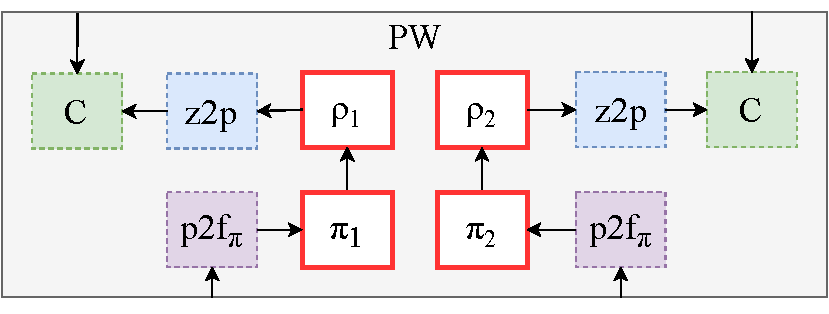
\includegraphics[scale=0.5]{figures/replacement2.pdf}
\caption{When we compose protocols we replace the \emph{p2f} process of $\rho$ with the corresponding instance of $\pi$ and its \emph{p2f} processes. By the emulation theorem, the channel offered by $\rho$ and accepted by $\pi$ have the same type.}
\label{fig:replacement}
\end{figure}

The code for the operator has the same type as any other protocol except, from the description above, it's offered channel is for the type of the functionality $\F_1$ instead of $\F_2$.
We rely on the code generation for to handle spawning instaces of a \inline{p2f} process corresponding to $\pi$ rather than $\rho$.
The operator is given in Figure~\ref{lst:compose}.
\begin{figure}
\begin{lstlisting}[basicstyle=\footnotesize\BeraMonottFamily, frame=single, mathescape]
$\tb{proc}$ compose[K][z,p]:
  (pid: Int), (rng: [Bit]), (sid: session[1]),
  (pid: Int), ($\$$z2p: z) |- ($\$$c: p) =
{
  $\$$ch <- PS.rho <- k rng sid pid $\$$z2p ;
  $\$$c <- Ps.pi <- k rng sid pid $\$$ch 
}
\end{lstlisting}
\caption{The composition operator accepts the same parameters as any other protocol party and offers the channel of type $p2f$ of the realizing protocol $\pi$. We connect $\rho$ to $\pi$ as an environment giving input to $\pi$. We do not need to include any import in our composition operator as the two protocols are guaranteed to be well-matched by the emulation definition. The operator replaces only one party (one \msf{pid}), and the \partywrapper instantiates parties that run the composed protocol.}
\label{lst:compose}
\end{figure}

The resulting composition operator, which composes the two simulators \SIM{\rho} and \SIM{\pi} inside the construction simulator, is best described in text as the resulting code is too verbose to include in the main body of this paper.
You can find the full simulator composition operator in the appendix.
\begin{itemize}
	\item Input from \Z is split between the two simulators
	\begin{itemize} 
		\item \inline{Z2A2P(pid, msg)} intended for parties of $\rho$ are passed to \SIM{\rho}
		\item \inline{Z2A2F(msg)} intended for $\F_1$ is passed to \SIM{\pi}.
	\end{itemize}
	\item Output from \SIM{\pi}: 
	\begin{itemize}
		\item \inline{A2F(msg)} for $\F_2$ and \inline{A2P(pid,msg)} for dummy parties of $\F_2$ are sent to \SIM{\rho} as \inline{Z2A2F(msg)}
		\item \inline{F2A2Z(msg)} is sent to \Z unaltered.
	\end{itemize}
	\item Output from \SIM{\rho}: 
	\begin{itemize}
		\item \inline{A2F(msg)} and \inline{A2P(pid,msg)} for $\F_3$ are sent out unaltered.
		\item \inline{F2A2Z(msg)} messages are sent to \SIM{\pi} as \inline{F2A(msg)} from $\F_2$.
		\item \inline{P2A2Z(pid,msg)} messages are sent to \Z unaltered.
	\end{itemize}
\end{itemize}
The simulator relies on simulators for $\F_1 \xrightarrow{\pi} \F_3$ and $\F_2 \xrightarrow{\rho} \F_3$ to satisfy simulation for Theorem~\ref{thm:singlecomp}.
It is clear that this construction adequately simulates the composed protocol. 
The type in the ideal world gurantees that both the real and ideal world adversaries get at least as much impor as any of the protocol parties. 
This ensures that the composed simulator has enough import to sandbox the two existing simulators and send import out to the ideal world parties and ideal funfctionality.
Therefore it is trivial to see that the composed simulator is well-resource-typed.

Another illustrative description of what composition proposes, logically, is shown by this series of UC executions where the $\equiv$ operator denotes equivalent UC executions that result from moving ITMs in and out of a sandbox, and $\approx$ indicates emulation:
\begin{align}
& \msf{execUC} \: \Z \, (\rho \circ \pi) \, \F_1 \, \DA \\
\equiv \; & \msf{execUC} \: (\Z \circ \rho) \, \pi \, \F_1 \, \DA \\
\approx \; & \msf{execUC} \: (\Z \circ \rho) \, \idealP \, \F_2 \, \SIM{\pi} \\
\equiv \; & \msf{execUC} \: \Z \, \rho \, \F_3 \, (\SIM{\pi} \circ \SIM{\rho})
%\approx \; & \msf{execUC} \: (\Z \circ \Sim{\pi}) \, \idealP \, \F_3 \, \Sim{\rho} \\
%\equiv \; & \msf{execUC} \: \Z \, \idealP \, \F_3 \, (\Sim{\pi} \circ \Sim{\rho}) 
\end{align}

%\item Inputs from \Z of \inline{Z2A2P(msg)} are passed to \SIM{\rho}, and inputs of \inline{Z2A2F(msg)} are passed to \SIM{\pi}.  
%\item \inline{P2A2Z(pid, msg)} outputs from \SIM{\rho} are forwarded to \Z unaltered.
%\item \inline{A2F(msg)} and \inline{A2P(pid, msg)} messages from \SIM{\pi} for $\F_2$ are sent to \SIM{\rho} as \inline{Z2A2F(msg)} and \inline{Z2A2P(pid, msg)}, respectively. 
%\item In the reverse direction, \inline{F2A2Z(msg)} messages from \SIM{\rho} are sent to \SIM{\pi} as \inline{F2A(msg)}, and, finally, \inline{F2A2Z(msg)} output generated by \SIM{\pi} is forwarded to \Z.
%\item \inline{A2P(pid,msg)}, \inline{A2F(msg)} messages from \SIM{\rho}, and \inline{P2A(pid,msg)} and \inline{F2A(msg)} from $\F_3$, are forwarded unaltered. 
%\end{itemize}

%We also provide a composition operator for simulators to construct a simulator for the composed protocol. We connect the simulatorsin the following way
%\begin{figure*}
%\begin{lstlisting}[basicstyle=\small\BeraMonottFamily, frame=single, mathescape]
%$\tb{proc}$ sim_compose[K][a2r,r2a][a2p,p2a][a2f,f2a]:
%  (k: Int), (rnd: [Bit]), (sid: session[1]),
%  (#z_to_a: comm[z2amsg[a2r][a2f]]), (#a_to_z: comm[a2zmsg[r2a,f2a]]),
%  (#a_to_p: comm[a2pmsg[a2r]]), (#p_to_a: comm[p2amsg[r2a]]), (#a_to_f: comm[a2fmsg[a2f]]), (#f_to_a: comm[f2amsg[f2a]])
%    |- ($\$$c: 1) =
%{
%  $\$$ch 
%\end{lstlisting}
%\end{figure*}

%\begin{figure*}
%\begin{lstlisting}[basicstyle=\small\BeraMonottFamily, frame=single,  mathescape]
%$\tb{proc}$ compose[K][z2r][r2z][f2r][r2f][p2f][f2p] : 
%    (pid: Int), ($\$$z_to_p: c[K][z2p]), ($\$$p_to_z: c[K][r2z]), 
%    ($\$$f_to_p: c[K][f2r]), ($\$$p_to_f: c[K][r2f])  |- ($\$$D : 1) =
%{
%	$\$$rho_to_pi <- $\tm{createchan}$[K][p2f];
%	$\$$pi_to_rho <- $\tm{createchan}$[K][f2p];
%
%	 <- pi  <-                 $\$$rho_to_pi $\$$pi_to_rho $\$$p_to_f $\$$f_to_p ;
%	 <- phi <- $\$$z_to_p $\$$p_to_z $\$$rho_to_pi $\$$pi_to_rho ; 
%}
%\end{lstlisting}
%\caption{Composition operator in Nomos that connects a protocol $\rho$ to a protocol $\pi$ that uses some functionality $\F$. The operators creates new channels to connect the realizing $\pi$ and it's hybrid \F. Output from $\rho$ intended for the replace functionality are actually send to parties of $\rho$, and channels outgoing from the parties to the functionality are given to $\pi$.}
%\label{lst:compose} 
%\end{figure*}

%\begin{theorem}[Composition]\label{thm:singlecomp}
%\begin{mathpar}
%\inferrule*[right=single-compose]
%{
%	\F_1 \xrightarrow{\pi} \F_2 \semi \F_2 \xrightarrow{\rho} \F_3 \\
%}
%{
%	\F_1 \xrightarrow{\rho \circ \pi} \F_3
%}
%\end{mathpar}
%
%If \textit{well-typed} $(\pi, \F_1$) realizes $\F_2$ and ($\rho$, $\F_2$) realizes some $\F_3$, then $(\rho \circ \pi, \F_2)$ is \textit{well-typed} and realizes $\F_3$ when $\circ$ is defined as in Figure~\ref{lst:compose}.
%\end{theorem}

%\begin{proof}
%The pre-condition ensures the existence of \textit{well-resource-typed} simulators $\Sim_\rho$ for $\F_2 \xrightarrow{\rho} \F_3$ and $\Sim_\pi$ for $\F_1 \xrightarrow{\pi} \F_2$, and, it is obvious that the composed protocol is also well-resource-typed.
%We construct a simulator \Sim' for the dummy adversary to show
%\[
%	\msf{execUC}\ (\rho \circ \pi)\ \F_1\ \Z\ \A \approx \msf{execUC}\ \idealP\ \F_3\ \Z\ \Sim''
%\]	
%
%The simulator $\Sim'$ relies only simulating \SIM{\pi} and \SIM{\rho}.
%Note that \SIM{\pi} can accept messages for $\pi$ or $\F_1$, simulate them, and generate input for $\F_2$. 
%Similarly, \SIM{\rho} can take inputs for $\rho$ or $\F_2$, simulate them, and generate input for $\F_3$.
%Therefore, we connect the two simulators in the natural way:
%\begin{itemize}
%\item Inputs from \Z of \inline{Z2A2P(msg)} are passed to \SIM{\rho}, and inputs of \inline{Z2A2F(msg)} are passed to \SIM{\pi}.  
%\item \inline{P2A2Z(pid, msg)} outputs from \SIM{\rho} are forwarded to \Z unaltered.
%\item \inline{A2F(msg)} and \inline{A2P(pid, msg)} messages from \SIM{\pi} for $\F_2$ are sent to \SIM{\rho} as \inline{Z2A2F(msg)} and \inline{Z2A2P(pid, msg)}, respectively. 
%\item In the reverse direction, \inline{F2A2Z(msg)} messages from \SIM{\rho} are sent to \SIM{\pi} as \inline{F2A(msg)}, and, finally, \inline{F2A2Z(msg)} output generated by \SIM{\pi} is forwarded to \Z.
%\item \inline{A2P(pid,msg)}, \inline{A2F(msg)} messages from \SIM{\rho}, and \inline{P2A(pid,msg)} and \inline{F2A(msg)} from $\F_3$, are forwarded unaltered. 
%\end{itemize}
%It is clear that \Sim' is able to emulate inputs from \Z to both parties of $\rho$ and the ideal functionalty $\F_1$.
%\Sim' performs constant over head in simulating two \emph{well-resource-typed}, and therefore it is clear that \Sim' is \emph{well-resource-typed}.
%When combined with the \emph{dummy lemma}, a well-resource-typed simulator exists for composition for any adverasry \A. 
%The dummy lemma presented above ensures that a simulator for any \A can be constructed that is well-resource-typed for all wel-resource-typed \A.
%\end{proof}
%
%We give a simpler, high-level idea of the forst step of the proof proof here which can be understood visually:
%The $\equiv$ operator is a result of moving around ITMs (some from within other ITMs into the main UC execution) and $\sim$ refers to indistinguishability.
%In line (13) above, $\rho$ is moved into the execution environment with an unchanged simulator as no additional simulation is required: the simulator allows unfettered communication between parties of $\rho$ and \Z.

\subsection{Multisession}

\begin{theorem}[Composition]\label{thm:composition}
\begin{mathpar}
\inferrule*[right=compose]
{
	%(\pi, !\F_1) \sim (\idealP, F_2) \semi (\rho, !\F_2) \sim (\idealP, \F_3) \\ 
	!\F_1 \xrightarrow{\pi} \F_2 \semi !\F_2 \xrightarrow{\rho} \F_3 \\
	%\Rightarrow \exists \Sim(\A) \vdash (\rho^{!\F_2 \rightarrow (!\pi \, \circ \, \msf{squash})}, !\F_1) \sim (\idealP, \F_3)
}
{
	!\F_1 \xrightarrow{\rho \, \circ !\pi \circ \, \msf{squash}} \F_3
	%(\rho \, \circ \, !\pi \circ \msf{squash}, !\F_1) \sim (\idealP, \F_3)
}
\end{mathpar}
\end{theorem}
Full composition in the UC framework extends beyond the simpler composition in Theorem~\ref{thm:singlecomp} which only defines replacement of one functionality with a protocol that realizes it.
Instead, UC composition allows for replacement of any number of instances of a functionality with instancesof the realizing protocol.
Theorem~\ref{thm:composition} illustrates the full composition theorem using our arrow notation, and highlights a theorem that we must prove before we can achieve full composition.
It relies on Theorem~\ref{thm:squash} that introduces the \msf{squash} protocol and the $!$ operator.
Notice that Theorem~\ref{thm:compose} follows directly from Theorem~\ref{thm:singlecomp} and Theorem~\ref{thm:squash}.

The multi-session extension of a protocol or functionality, specified by the $!$ operator (such as $!\rho$ or $!\F$), allows multiple instances of the protocol/functionality to be run within a sinlge ITM.
An ITM simulates the instances and multiplexes input/output to/from them much like the \partywrapper.

\begin{theorem}[Squash Theorem]\label{thm:squash}
%If a functionality \F is well-resource-typed, then $!\F$ and $!!\F$ are well-resource-typed (by Theorem~\ref{thm:bangppt}) and $(\idealP, !!\F) \sim (\msf{squash}, !\F)$.
%\textit{Well-resource-typed} \F $\Rightarrow$ $!\F \xrightarrow{\msf{squash}} !!\F$%  $(\idealP, !!\F) \sim (\msf{squash}, !\F)$
\begin{mathpar}
\inferrule*[right=squash]
{
\textit{well-resource-typed} \; \F
}
{
!\F \xrightarrow{\msf{squash}} !!\F
}
\end{mathpar}
\end{theorem}

For the multisession extension of a fuctionality, the type is straightforward and ony acts to multiplex input/outpt based on the intended target \inline{ssid}.
\begin{center}
\parbox{0cm}{
\begin{tabbing}
$\m{{P2MS}[a,b]\{n,m\}} = \textcolor{red}{\getpot^n} \ichoice{\mb{Inp}: ssid \arrow a \tensor \echoice{$\=$\mb{Ok}: \textcolor{red}{\paypot^0} \; \m{P2MS[a,b]\{n,m\}},$ \\
\>$\mb{Out}: ssid \arrow b \tensor \textcolor{red}{\paypot^m} \; \m{P2MS[a,b]\{m,n\}}}}$
%\m{MS2P[a][b]\{n,m\}}}$ \\
%\mi{stype} \; \m{{MS2P}[a][b]\{n,m\}} = \echoice{\mb{Ok}: \textcolor{red}{\paypot^0} \; \m{P2MS[a][b]\{n,m\}}, \mb{Out}: ssid \product b \arrow \textcolor{red}{\paypot^m} \; \m{P2MS[a][b]\{n,m\}}}  
\end{tabbing}}
\end{center}
The multisession extension is mentioned in greater detail in the appendix.
%and the functional types that are sent to the wrapper surrounding it are given by
%\begin{lstlisting}[basicstyle=\small\BeraMonottFamily, mathescape]
%$\yo{type}$ p2ms[a] = P2MS of ssid ^ a ;
%$\yo{type}$ ms2p[b] = MS2P of ssid ^ b ;
%\end{lstlisting}
%It is important to note that we require a session type here instead of allowing !\F act as the functionality wrapper because, when composed it must communicate directly communicate, over a session-typed channel, to another protocol.
%Furthermore, the construction of !\F is the same as in the \Fro example: one session typed channel for all parties.
%In Figure~\ref{fig:multisession} illustrated the functionality wrapper (right) and the multisession extension (left) for \Fcom. 
%\begin{figure}
%\centering
%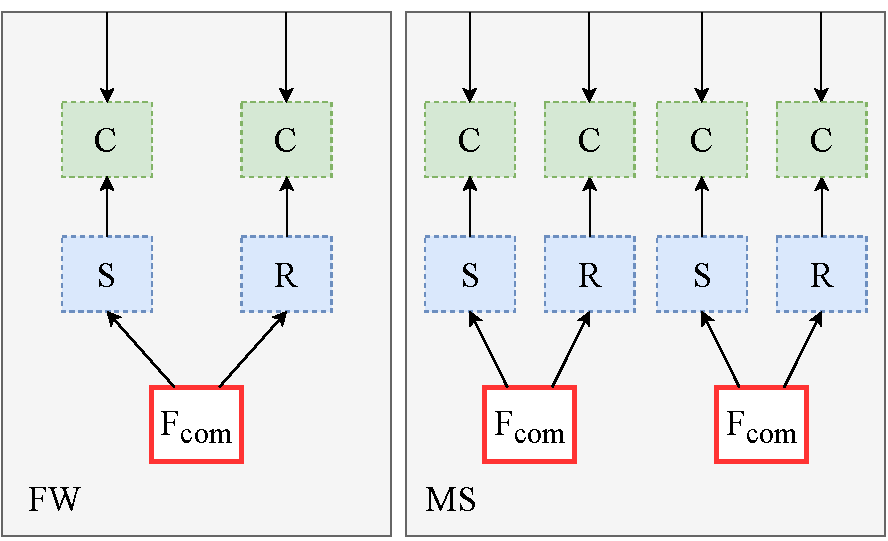
\includegraphics[scale=0.5]{figures/multisession.pdf}
%\caption{The multisession extension of \Fcom (right) with only two instances, creates the same processes $S$ and $R$ (offering the session typed channel to \Fcom) for every created instance. A communicator per session buffers messages for the $S$ and $R$ processes to consume and forward along their session-typed channel to \Fcom.}
%\label{fig:multisession}
%\end{figure}

%As a generic construction provided by NomosUC, the multisession operator requires some code generation but only to accept an arbitrary number of virtual token types if the underlying \F simulators other processes. 
%Furthermore, similar to the functionality wrapper, the multisession operator constructs the processes around \F in the same way and spawns them on-demand.
%The process definition for $!\F_\msf{com}$ is shown in Figure \ref{lst:bangf} accepting two token types: the real token type $K$ and the virtual token type $K_1$ for instances of $\F_\msf{com}$.
%
%\begin{figure}
%\begin{lstlisting}[basicstyle=\footnotesize\BeraMonottFamily, frame=single, mathescape]
%$\tb{proc}$ bangF[K,K1][p2f,...] :
%  (k: $\tgr{Int}$), (rng: [Bit]), (sid: session[a]), 
%  ($\$$p: P2MS[p2f][f2p]) |- ($\$$ch: 1) =
%\end{lstlisting}
%\caption{The type definition for the multisession operator for functionalities and the correspond message type and import parameters. The operator for protocol parties is identical in code but differens in that the parameters to the \texttt{P2MS} type are for \texttt{Z2P} interaction.}
%\label{lst:bangf}
%\end{figure}

\begin{theorem}[PPT !]\label{thm:bangppt}
If a functionality $\F$ is well-resource-typed, then it's multisession extension $!\F$ is well-resource-typed.
\end{theorem}

We examine this theorem in greater detail in the appendix. 
At a high-level it is obvious that such a construction, activated polynomially many times, is well-resource-typed as long as the underlying functionality/protocol is well-resource-typed.
%\begin{proof}
%A \textit{well-resource-typed} \F guarantees a polynomial $T_{\F}$ bounding its execution.
%In the worse-case, the multisession operator must spawn a new instance of $\F$ an every activation. 
%Let $N_{\F}$ denote the total number of instances (and, hence, number of activations) of $\F$ created by the operator.
%Note that $N_{\F}$ is polynomial in the security parameter $k$ for all well-typed environments, protocols, and adversary.
%Therefore, there always exists a bounding polynomial to bound a polynomial number of simulated instances of \F.
%The polynomial can be given as:
%$$ P_{!\F}(n) = N_{\F} P_{\F}(n) + \mathcal{O}(N_{\F}) $$
%where the $\mathcal{O}(N_{\F})$ is due to the overhead of maintaining and accessing the set of all instances.
%
%Similarly, \F being \textit{well-resource-typed} ensures a valid token context for all processes it may simulate. 
%Therefore, it is clear that there exists a global connecting poltnomial $f$ that ensures a valid token context for $!\F$.
%\end{proof}


%\begin{figure}
%\begin{lstlisting}[basicstyle=\small\BeraMonottFamily, mathescape, frame=single]
%$\yo{type}$ p2bFmsg[a] = P2bF of ssid ^ a ;
%$\yo{type}$ p2bbFmsg[a] = P2bbF of ssid ^ ssid ^ a ;
%$\tg{(* z2p : comm[z2pmsg[p2bbf[a]]] *)}$
%$\tg{(* p2f : comm[p2fmsg[P2bf[a]]] *)}$
%pid = recv $\$$z2p ;
%m = recv $\$$z2p ;
%case m (
%  P2bbF(ssid1, ssid2, m) =>
%    send $\$$p2f P2bF(ssid1 + ssid2, m) ;
%)
%\end{lstlisting}
%\caption{The \textit{squash protocol} accepts a message intended intended for $!!\F$ of type \inline{P2MS[p2ms[a]][ms2p[b]]}, i.e. of the form $(\msf{ssid}_1, (\msf{ssid}_1, msg))$.
%It ``flattens'' it into a single $\msf{ssid}_3 = \msf{ssid}_1 + \msf{ssid}_2$ that can be passed to $!\F$. The result is the same number of instances of \F but behind only a single $!$ operator.}
%\label{fig:squash}
%\end{figure}

\begin{proof} (Theorem~\ref{thm:squash})
On examination the \msf{squash} theorem does constant work per activation and concantenates two \inline{ssid}s into one for messages going to the functionality and does the inverse for messages incoming from the functionality.
We provide more detail for a proof of Theorem~\ref{thm:squash} in the Appendix, however, it is clear to see that the this theorem holds with a trivial simulator.
%First we describe the \msf{squash} protocol where $!!\F$ are nested $!$ operators.
%The protocol accepts messages intended for $!!\F$ of type \inline{P2MS[p2ms[a]][ms2p[b]]}, i.e. of the form $(\msf{ssid}_1, (\msf{ssid}_2, msg))$, and ``flattens'' them into a single message of type $\inline{P2MS[a][b]}$, i.e. of the form $(\msf{ssid}_3, msg)$.
%
%In $(\idealP, !!\F)$, \idealP~expects to receive messages of the form $(\msf{ssid}_1, (\msf{ssid}_2, m))$ where $\msf{ssid_2}$ is a sub-session of $\F$ (i.e. instance) inside some $!\F$ with sub-session id $\msf{ssid}_1$ inside of $!!\F$ (the message accesses functionality $\F[\msf{ssid}_1][\msf{ssid}_2]$).
%The \msf{squash} protocol flattens the indexing of instances of \F and combines session ids $\msf{ssid}_1$ and $\msf{ssid}_2$ into a single \msf{ssid}: $\msf{ssid}_3 := \msf{ssid}_1 \cdot \msf{ssid}_2$.
%If follows intuitively that the view for the environment remains the same. 
%
%We construct a simulator such that:
%\[
%\msf{execUC} \, \Z \, \idealP \, !!\F \, \SIM{\msf{squash}} \approx \msf{execUC} \, \Z \, \msf{squash} \, !\F \DA 
%\]
%The simulator is very simple. 
%Inputs to/from parties/\Z for a corrupt party is forwarded unmodified.
%Input intended for $!\F$ of the form $(\msf{ssid}_1 \cdot \msf{ssid}_2, msg)$ is sent as $(\msf{ssid}_1, (\msf{ssid}_2, msg))$ to $!!\F$. 
%Output from $!!\F$ is modified inversely and sent to \Z.
%
%The proposed simulator is trivially analyzed to be \textit{well-resource-typed}.
%It performs constant work per activation and does ``real'' simulation other than message modification to/from $!!\F$.
\end{proof}

\subsection{UC Composition}
Finally, we can conlude with full composition in Theorem~\ref{thm:compose}.
The proof follows directly from Theorems~\ref{thm:singlecomp} and \ref{thm:squash}.

\begin{proof}
By Theorem~\ref{thm:singlecomp} we can construct a simulator \SIM{1} for $!!\F_1 \xrightarrow{\rho \, \circ \, !\pi} \F_3$.
Theorem~\ref{thm:squash} then allows us to ``squash'' $!!\F_1$ and construct a simulator using \SIM{1} for $!\F_1 \xrightarrow{\rho \, \circ \, !\pi \, \circ \, \msf{squash}} \F_3$
\end{proof}

\subsection{Design Discussion}
One of the core research questions that this work aims to study session types applied to the UC framework. 
In this section, we discuss how resource-aware session types impact the design of functionalities in NomosUC as well as which are implementable.
We use the two-way authenticated channel functionality \Fauth to througout this discussion.

In plain session types, communication between two parties $P_s$ and $P_r$ occurs over a single duplex channel.
In UC the role of the adversary as a message scheduler in \Fauth, the most common network channel model, means a more complicated functionaty involving $P_s$, $P_r$, \F, and \A. 
The simplest, and most common approach, to \Fauth is the following communication pattern: a party $P_s$ sends a message to \Fauth, \Fauth sends the message to \A and waits for \A to say \inline{OK} before delivering the message to $P_r$.
Since both parties can send a message and receive a message, it is unclear which process, \Fauth or $P$, will be active along that channel at any given time.
Session types require this information to be statically known when two processes are communicating over a single channel--making this communication pattern unexpressable over a single channel.

There a few ways to overcome this constraint. 
In general, even though the UC framework places few restructions of communication patterns, most functionalities stick to a few.
\Fauth, for example, can take a few forms:
\begin{enumerate}
\item (presented above) Receiver and adverasry are activated directly: \Fauth waits for \A to tell it to deliver the message.
\item \Fauth ``polling'' approach: messages from $P_s$ are buffered for both \A and $P_r$. \A and $P_r$ must ask \Fauth for new messages. This is a more invonconvenient method, but can be useful for novel functionality designs that need a channel.
\item ``polling'' but receiver is activated: the message is stored in a buffer for \A, and \A's deliver message directly sends it to $P_r$.
\end{enumerate}
The simplest way to implement \Fauth in NomosUC is ``polling'' approach. As far as we know, we can systematically tranform any UC functionality into one that uses ``polling''. 
The consequences are that polling is inconvenient from a programming point of view because \Z needs to continuously activate parties to ask for new messages.
Hope is not lost though, because it turns out our type system can express functionalities in all three of the ways listed above. 
The first, and most natural, approach only requires splitting communicating between $P$ and \Fauth into two unidirectional channels
Such an extension to NomosUC trivially modifies the \partywrapper to handle two channels instead of one, and the types of the channels can be succintly expressed as: 
\begin{center}
\parbox{0cm}{
\begin{tabbing}
$\m{sending}[a] = \textcolor{red}{\getpot^n} \ichoice{\mb{sendmsg}: \m{a} \tensor \m{sendmsg}}$ \\
$\m{receive}[a] = \textcolor{red}{\getpot^m} \echoice{\mb{recv}: \m{a} \tensor \m{receive}}$ \\
$\m{adv}[a] = \echoice{\mb{leakmsg}: a \tensor \ichoice{ \mb{ok}: \m{leakmsg}}}$
\end{tabbing}}
\end{center}
The first to correspond to the channels for sending from $P$ to \Fauth and the second in the opposite direction. The third is the adversary's channel at \Fauth.

A notable part of our contruction is the machinery created around the protocol parties and functionality that intemediate their communication with communicators and functionally-typed messages.
Recall that such compromises are required in order to allow a \emph{dynamic} number of parties in UC.
The session type of the shared channel of a communicator only allows for a fixed amount of import to be sent over it with every messages. 
Protocols and functionalities that send different amounts of import depending on the message, say $i_1,...,i_n$, must now send $\m{max}(\{i_j\})$ import with every messages.
For existing UC definitions this appears to be an issue of ensuring a machine has \emph{enough} import, however, we can systematically map any UC import definition to one that works in NomosUC~\footnote{The problem can be reduced to ensuring enough ``latent'' import needed to compute, and, because we aren't concerned here with \emph{tight} computational bounds the problem is quite easy to solve. We discuss in greater detail in the appendix.}.



%\caption{The \msf{execUC} function used for the two-party commitment example used througout this paper. Recall, the \msf{execUC} is customized insofar as it takes in some number of virtual token types (here, $K_1$) to enable machines that simulate other machines. In the commitment example, there is no such simulation happening at the protocol or functionality level, therefore only the real token type $K_1$ is used here. The funtion spawns all the necessary ITMs in the UC execution: the environment, the protocol wrapper, the functionalty (wrapped), and the adversary. Each is parameterized with the security parameter $k$ and a random bit sequence $\msf{rng} \in \{0,1\}^{poly(k)}$.
%At the end, the environment is started and it returns a bit $b$ which is its guess for which world it is in. The full code can be found in the Appendix.}
%\label{lst:execuc}
%\end{figure*}

%We separate NomosUC into two modules: generic code and protocol-specific code. 
%Therefore, the \inline{execUC} refers to user specified code through the \inline{PS} module which defines \inline{PS.env} for \Z, \inline{PS.func} for the functionality, \inline{PS.prot} for the protocol, and \inline{PS.adv} for the adversary.
Communication between all of the major processes in the UC execution (\Z, \A, \partywrapper, and \fwrapper) is done through communicators introduced in Section~\ref{sec:nomosuc}.
Communicators are restricted to only sending functionally types messages in NomosUC, and we give generic types, below, to all such messages.
\todo{Is this important to even have here? seems a useless implementation detail.}
\begin{lstlisting}[basicstyle=\footnotesize\BeraMonottFamily, frame=single, mathescape]
$\Type$ p2zmsg[a] = P2Z of pid ^ a ;
$\Type$ p2fmsg[a] = P2F of pid ^ a ;
$\Type$ f2pmsg[a] = F2P of pid ^ a ;
\end{lstlisting}

\paragraph{The Environment}
The environment is the first machine that \inline{execUC} spawns and receives from it the session id and list of corrupted parties for this execution.
Its offered channel type \inline{EtoZ} specifies the interaction between \inline{execUC} and \Z:
\begin{lstlisting}[basicstyle=\footnotesize\BeraMonottFamily, mathescape, frame=single]
$\Type$ EtoZ[a] = +{init: a ^ list[pid] -> exec} 
$\Type$ exec = &{start : output_bit} ;
$\Type$ output_bit = +{bit: Bit -> 1} ;

$\tb{proc}$ PS.env[K][z2p,...]{p2zn,...} : 
  (k: $\tgr{int}$), (r: [Bit]), (#ztop: comm[z2pmsg[z2p]]{z2pn}), 
  (#ptoz: comm[p2zmsg[p2z]]{p2zn})...  |- ($\$$z : EtoZ) $\tg{(* <- offered channel *)}$
\end{lstlisting}
The environment also accepts communicators, as parameters, for communication with the protocol parties and the adversaries (in both directions), and offer a channel \inline{$\$$z} of type \inline{EtoZ}.
The type (above) states \Z provides an \emph{sid} of some user-defined type \inline{a} and a list of the \emph{pid}s of corrupted parties. 
Finally, \inline{execUC} instructs it to \inline{start} (\emph{external choice}) and return a bit $b$ as its guess for which world it is in.

%The \inline{\{z2pn\}}, for example, specifies the amount of import that must be sent by \Z with every message to a protocol party.
%The rest of the processes---the adversary, protocol wrapper, and functionality--are declared in the same way except the type parameters they expect are different: the protocol wrapper would of course accept type parameters for communication between it and \F, \A, and \Z.
%Finally the type of the offered channel \inline{$\$$z} is the same for all environments and communicates the \inline{sid} and set of corrupt parties chosen by \Z to \inline{execUC}.
%The \inline{sid} and corrupt list are parameters to the rest of the processes that \inline{execUC} spawns. 

%The communicators created by \inline{execUC} always use the same parametric types. 
%For example, for communication with the protocol, the types look like:
%\begin{lstlisting}[basicstyle=\small\BeraMonottFamily, frame=single, mathescape]
%$\Type$ p2zmsg[a] = P2Z of pid ^ a ;
%$\Type$ p2fmsg[a] = P2F of pid ^ a ;
%$\Type$ f2pmsg[a] = F2P of pid ^ a ;
%\end{lstlisting}
%Subsequently, the channel from \Z to the protocol wrapper will be typed as: \inline{comm[z2pmsg[z2p]]\{z2pn\}} where \inline{z2p} is a protocol-specific message type.
%The protocol \inline{PS.prot} is not spawned by \inline{execUC}. Instead the process spawns the protocol wrapper (described below) which spawns parties with that run the code \inline{PS.prot}.
%When in the ideal world, the protocol is given as the ideal protocol: one where the protocol wrapper converts the message from type \inline{z2pmsg[a]} to type \inline{p2fmsg[a]} but forwards the contents unaltered.
%The protocol wrapper and functionality wrapper manage spawning the instance(s) of the functionality and protocol parties.
%Similarly, an environment \msf{PS.env} and adversary \msf{PS.adv} must be defined as well.
%The message types exchanged between the processes are provided directly to \msf{execUC} as type parameters of the form \msf{p2f}, \msf{f2p}, and so on. 
%The first thing \inline{execUC} does is create the communicators and the corresponding channels for the main processes of the execution. 

%A consequence of using communicators is that in the UC setting they require at least 1 unit of import, beacuse they are activated a potentially polynomial number of times. 
%Therefore, all communicators in NomosUC receive some amount of import $n$ and send out only $n-1$. 
%The user-specified protocol, environment, functionality, and adverasary must account for this to ensure suffiient import is given to them.
%\begin{lstlisting}[basicstyle=\small\BeraMonottFamily, frame=single, mathescape]
%#ptoz <- communicator_init[K][p2zmsg[p2z]]
%           {p2zn+1} ;
%#ztop <- communicator_init[K][z2pmsg[z2p]]
%           {z2pn+1} ;
%...
%\end{lstlisting}
%This is strictly a design decision where user-defined protocols only specify import token requirements for the protocol not taking communicators into account. 
%The processes that they write, though, must conform to this standard and send an import token in addition to the amount they need.
%An alternate design would be that all import type parameters take the additional import token into account and communicators send one less than they receive.
%The drawback of the latter approach is that that when communicating with a process directly rather than through communicators (say, when simulating), you're sending one extra token for no reason.

%Next, the environment \msf{PS.env} is spawned, \inline{execUC} receives the \inline{sid} and corrupt list from \Z, and, finally, the remainder of the processes are spawned with these inputs. 
%Finally, the environment executes its own code when activated by \msf{\$z.start}, given the initial amoutn of import \inline{n}, and returns a bit through \inline{$\$$z.output_bit} which is its guess whether it's in the real or ideal world:
%\begin{lstlisting}[basicstyle=\small\BeraMonottFamily, frame=single, mathescape]
%$\$$z.start
%$\tb{pay}$ $\$$z {n}
%$\$$d <- $\$$z
%\end{lstlisting}

\subsection{The \partywrapper}
NomosUC departs slightly from the standard UC framework by using a \partywrapper to encapsulate all protocol parties and run them internally.
Rather than passing protocol party channels as parameters to \Z or \A (supporting a static set of parties), the \partywrapper provides a single endpoint for all messages to parties.
Similarly we adapt a \fwrapper to function like the \partywrapper but on functionalities. The main pupose of this wrapper and the \partywrapper is to intermediate communication between the session types the functionality uses and the functionally typed messages exchanges through communicators.

Like \iexecuc, we genrate the \partywrapper based on the protocol or functionality being executed. 
Converting between functional and session-typed messages is an easy task to automate and we push that onto code generation rather than requiring a user to produce it.
The extra processes generated within the \partywrapper are shown in Fiure~\ref{fig:blankpartywrapper}.
%In a nutshell, the wrapper accepts messages from a communicator, say from \Z, demultiplexes it, converts its type to one over a session-typed channel and conveys it to the necessary protocol party.

Following along with Figure~\ref{fig:blankpartywrapper}, the generated processes \inline{C} are use to de-multiplex messages based on the \inline{pid} of the receipient, and the \inline{z2p} and \inline{p2f} processes convert messages between the session typed channels and the functional messages that are received.
The arrow notation in Figure~\ref{fig:blankpartywrapper} indicates the $\m{prodiver} \leftarrow \m{client}$ relationship for each channel and provides their types.

We elaborate on the processes \inline{z2p}. For the commitment protocol the messages received by the \partywrapper are type as 
\begin{lstlisting}[basicstyle=\footnotesize\BeraMonottFamily, mathescape]
$\yo{type}$ comp2f = Commit of Bit | Open ;
$\yo{type}$ comf2p = Committed | Open of Bit ;
\end{lstlisting}
and the \inline{z2p} process intercepts them and communicates to the party over a channel typed with the \Fcom session types in Section~\ref{sec:nomosuc}.
For example when \Z gives the command to commit to a bit, \inline{z2p} does the following:
\begin{lstlisting}[basicstyle=\footnotesize\BeraMonottFamily, frame=single, mathescape]
case msg (
  Commit(b) =>
    $\$$z2p.commit ;
    $\tb{send}$ $\$$z2p b ;
    $\tb{pay}$ {z2pn} $\$$z2p ;
\end{lstlisting}
where \inline{$\$$z2p} is the session-typed channel to the committer.
The \inline{f2p} processes does the same for communication between the parties and the functionality.

Virtualizing the protoocl parties means that the wrapper and the parties it runs are, effectively, using the same import and potential.
We reason that the \partywrapper and protocol parties it runs will always have enough import by noticing that the \partywrapper does constant work on each activation.
Therefore, if protocol parties intend to hold on to import, there is always a suficient polynomial to allow both the wrapper and the party to perform potentially polynomial computation.
\todo{Reword this to make it crisper}.

%Folling along with Figure~\ref{fig:blankpartywrapper}, the generatd processes \inline{z2p} and \inline{f2p} communicate with the party over a session-typed channel and perform the message type conversion mentioned above based on a simple message type mapping provided by the user.
%The \inline{z2p} process offers a linear channel to the party with the correct session type with \Z. 
%The wrapper reads messages from \Z, demultiplexes them based on \inline{pid} and puts them in the appropriate virtual communcator (the green box labeled \inline{C}) for the \inline{z2p} processes to read from, convert, and send to the party.
%The protocol party offers a linear channel of its type with \F, and \inline{p2f} converts this to a functional type. \inline{p2f} offers the same type as a communciator to the wrapper which reads the message and sends it to \F. 
%Figure~\ref{fig:blankpartywrapper} indicates the type of the offered channel for all the relevant processes within the wrapper. 

%In order to use session types, the each protocol party is internally connected to two processes \inline{z2p} and \inline{f2p} over with session-typed channels for their communication with \Z and \F, respectively.
%\inline{z2p} is connected to party-specific virtual communicators so that \inline{z2p} and \inline{f2p} can read/send messages from. It can not read/write directly to/from the actual communicators connecting the protocol wrapper because, being simulations inside the protocol wrapper, they do not use the same token type.
%In the case of the ideal world with \Fcom, the both of the sender's ($\pi_1$) channel with \inline{z2p} channels with \inline{z2p} and \inline{f2p} are typed as \inline{sender}, and the protocol party itself ($\pi_1$) just fowards messages from one channel to the other.

%The processes \inline{Z2p} and \inline{f2p} are generated for each party based on their session-type, and they convert between them and functional messages for incoming/outgoing communcation with \Z, \F, or \A. 
%For example in the commitment example, where the functional message type is given by: 
%\begin{lstlisting}[basicstyle=\footnotesize\BeraMonottFamily, mathescape]
%$\yo{type}$ comp2f = Commit of Bit | Open ;
%$\yo{type}$ comf2p = Committed | Open of Bit ;
%\end{lstlisting}
%the \inline{z2p} process does something like this for the sender (where \inline{msg} is received from its virtual communicator):
%\begin{lstlisting}[basicstyle=\footnotesize\BeraMonottFamily, frame=single, mathescape]
%case msg (
%  Commit(b) =>
%    $\$$z2p.commit ;
%    $\tb{send}$ $\$$z2p b ;
%    $\tb{pay}$ {z2pn} $\$$z2p ;
%\end{lstlisting}
%It sends a commit message over the linear channel with the sender, and pays the necessary amount of (virtual) import tokens with the message.
%When \Z, \A, or \F send a message to a party that doesn't exist, the \partywrapper creates the new party's \inline{z2p}/\inline{f2p} processes and an instance of the party itself, and it connects them together in the same way shown. 
%We do something similar for functionalities, in Appefix~\ref{app:fwrapper}

\begin{figure}
\centering
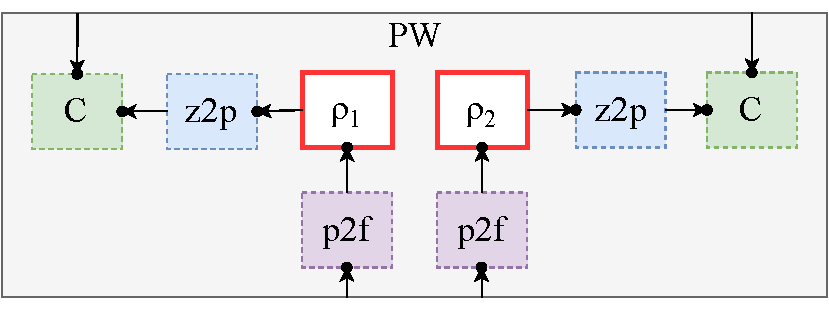
\includegraphics[scale=0.5]{figures/blankpartywrapper2.pdf}
\caption{The internals of the protocol wrapper with two parties. The arrows indicates the client/provider relationship between each pair: provider $\rightarrow$ client. The wrapper creates \texttt{z2p} to offer a channel and convert from gunctional to message type---the \texttt{p2f} do the same. A communicator is used because \texttt{z2p} cannot send message to real one with differing token type. The types of the processes offered are (color): \tgr{comm[z2pmsg[comp2f]]}, \tb{sender}, \tr{party[Int]}, \tp{comm[p2fmsg[rop2f]]}. }
%The processes \texttt{z2p} offer linear channels to their respective protocol parties that are typed according to that party's protocol, and they receive messages from virtual communicators that hold messages specific to one \texttt{pid}. The protocol code for $\pi_1$ and $\pi_2$ are user-specified and offer a channel to the \texttt{p2f} process according to their protocol with the functionality. The \texttt{p2f}s convert outgoing messages to, and incoming messages from, functional message types to be sent to/from the functionality. The protocol wrapper gives messages to the virtual communicators and receives messages from \texttt{p2f}s.}
\label{fig:blankpartywrapper}
\vspace{-1.5em}
\end{figure}

%For the commitment example, if $\pi_1$ and $\pi_2$ ran the commitment protocol, \inline{z2p} would offer a channel of type \inline{sender} and \inline{receiver} to $\pi_1$ and $\pi_2$, respectively, and it converts between the functional messages for the commitment protocol and the session typed ones. 
%In the ideal world, the $\pi_1$ and $\pi_2$ run a dummy protocol where their offered channels are simply forwarded to their \inline{z2p} channels, i.e. the \inline{z2p} and \inline{f2p} channels have the same type: \inline{sender} and \inline{receiver}, respectively.
%In the style of Nomos, the protocol wrapper:
%\begin{itemize}
%	\item Attempts to read messages incoming from \Z, \A, or \F and forward them to the appropriate process depending on \inline{pid}.
%	\item Read from the internal communicators or the \inline{p2f} processes for outcoing messages.
%\end{itemize}
%For reference the functional messages typed for the commitment protocol are:

%Recall the session types for the sender and receiver, with \Fcom, introduced in Section \ref{subsec:idealcommitment}.
%%\begin{gather}
%%	\mi{stype} \; \m{sender} = \ichoice{\mb{commit} : \m{bit} \product \m{scommitted}} \\
%%	\mi{stype} \; \m{scommitted} = \ichoice{\mb{open} : 1} \\
%%	\mi{stype} \; \m{receiver} = \echoice{\mb{commit} : \m{rcommitted}} \\
%%	\mi{stype} \; \m{rcommitted} = \echoice{\mb{open} : \m{bit} \arrow \one}
%%\end{gather}
%At the beginning there are no parties. When the \A or \Z write to a party with some pid $p$ the protocol wrapper creates $p$ if it does not exist.
%It creates and stores the session-typed channels or all of the parties in channels corresponding to their type and moves channels between them as the type evolves.
%For example for parties' channel with \Z the protocol wrapper generates the following lists:
%\begin{gather}
%	\m{R1L1}[\m{sender}] \\
%	\m{R1L2}[\m{scommitted}] \\
%	\m{R2L1}[\m{receiver}] \\
%	\m{R2L2}[\m{rcommitted}] 
%\end{gather}
%At the beginning of the protocol, the committer's \msf{z2p} channel would be in \inline{R1L1} and the receiver's is in \inline{R2L1}.
%The channel's connection the protocol wrapper to the rest are still functionally typed. It's channel \inline{p2f} will still be typed \inline{#ptof: comm[p2fmsg[comp2f]]} where \inline{comp2f} is:
%Succinctly, the protocol wrapper functions as follows:
%\begin{itemize}
%\item When the protocol wrapper receives a message for some \msf{pid}, if the party doesn't exist the protocol wrapper creates all the party's channel parameterized by the correct session types (the role of the party is determined by the incoming message). The channels are stored and outgoing channels are waiting to be read from.
%\item The message sent to the party with the session type is determined by the functional type. The wrapper creates a session-typed message and forwards the contents of the message to the party.
%Despite accepting functionally typed messages, the protocol wrapper uses session types in this way to allow the type checker to catch invalid and out of order environments, adversaries and functionalities. 
%For example, in the commitment protocol when the committer tries to commit a bit in \Fcom like this:
%\begin{lstlisting}[basicstyle=\small\BeraMonottFamily, frame=single, mathescape]
%$\$$p2f.commit 
%$\tb{send}$ $\$$p2f b
%$\tb{pay}$ {p2fn} $\$$p2f
%\end{lstlisting}
%\begin{lstlisting}[basicstyle=\small\BeraMonottFamily, frame=single, mathescape]
%$\$$p2f.SEND 
%$\tb{send}$ $\$$p2f pid 
%$\tb{send}$ $\$$p2f Commit(b)
%$\tb{pay}$ {p2fn} $\$$p2f
%\end{lstlisting}
%The party wrapper intercepts and converts it to a functionally typed message:
%\item For outgoing messages, the protocol wrapper does a similar conversion where it reads the sesion typed channel output by the party and converts its message to the appropriate functional message type.
%\end{itemize}

%\paragraph{Functionality Wrapper}
%The \fwrapper adopts a similar approach to the \partywrapper, except it only creates one instance of the underlying functionality.
%For the same reason as the \partywrapper, we use an \fwrapper to enable a dynamic set of parties.
%One caveat in supporting such functionalities, is that, so far, only functionalities whose type follows a specific form are allowed.
%In the random oracle type given below, notice that the type before and after a party interacts with it is the same: type $\m{party}[a]$.
%\begin{mathpar}
%\m{party}[a] = \textcolor{red}{\getpot^1} \ichoice{\mb{hash} : \m{pid} \arrow \m{int} \product \m{hashing}[a]} \\
%\m{hashing}[a] = \echoice{\mb{shash} : \m{pid} \arrow \m{int} \product \textcolor{red}{\paypot^0} \m{party}[a]} 
%\end{mathpar}
%A party queries a $\mb{hash}$ of an integer from \Fro and receives an integer as a response. The session type includes the \inline{pid}, which enables it to handle all parties over the same channel.
%
%An example of the internals of the \fwrapper are showing on the left-hand-side of Figure~\ref{fig:multisession}.
%Like the \inline{z2p} processes in the \partywrapper, \inline{S} and \inline{R} represent the sender and receiver in the commitment protocol, and they read from their virtual communicators and communicate with \Fcom over a session-typed channel.

%When a party invokes \Fro, the type it expects is \inline{party[a]}, and when it has received its hash the type is again back at \inline{party[a]}. 
%The wrapper handles such dynamic functionalities by channeling all party communication through one linear channel in the wrapper. 
%Therefore, \Fro reads on one channel and responds to the specific party with some \inline{pid}, and the protocol wrapper remains unchanged. 
%
%The constructions of the protocol wrapper and functionality wrapper enable users to write very simple ideal functionality and protocol code, as we will discuss in the next Section and in the Appedix.

%In the commitment example, \Fcom accepts two channels, one from each party, and two processes are created (call then \inline{p2f} for now) which offer channels of type \inline{sender} and \inline{receiver}, respectively. 
%The wrapper differs from the protocol wrapper for certain functionalities that accept a dynamic number of parties. 
%Continuing with our commitment example, the random oracle functionality, an idealized hash function, is used in the real world to realize \Fcom, and it allows a dynamic set of parties to inteact with it.
%Its session type with protocol parties is given below.
%The session type is special in that, for every interaction, the channels type always ends up back at \inline{party[a]} before any other party tries to use \Fro.
%NomosUC enables ideal functionalities whose types work like this by adding the \inline{pid} to the type, and having only one process in the functionality wrapper offering a channel of this type to \Fro.
%Unlike \Fcom where new communicator and \inline{p2f} process is created for each new party, messages from all parties pass through one such process.
%Additionally, moving the \inline{pid} into the session type means that the protocol wrapper can create arbitrarily many \inline{pid}s to communicate with \Fro.

\paragraph{The Adversary}
The adversary, much like the environment, is providing input to the protocol and functionalities.
As the UC framework is concerned with modular construction for protocols, and NomosUC with using session types to aid in suc construction, we do not give adversaries session types.
Therefore, they are not wrapper like protocols and functionalities, and communicate with all other processes directly through functional message types.

\subsection{Polynomial Bound}
The security of the UC framework relies on computational constraints on adversaries, and, generally, on what all ITMs can do.
It introduces the concept of import tokens as a new way to reason about ITMs being polynomial in the security parameter $k$. 
The import mechainsm as described in UC, and which we descrive in Section~\ref{sec:background}, ensures that a single ITM's execution is upper-bounded by some poynomial $T(n,k)$ where $T$ is a polynomial, $n$ is its net import token balance (received - sent), and $k$ is the security parameter.
Canetti et al. limit their discussion to parameterized systems where all machines do not do anything until they have received at least $k$ import.
We depart from this notion slightly and express ``interactive polynomial time'' by using a bounding polynomial in both import and $k$.
We do this for two reasons.
First, it remedies our exclusion of ``parameterized systems'' by easing the import requirements of cacnonical cryprograpic operations, such as a random oracle operation on $k$-bit strings that would otherwise require $k$ import. 
Second, we add $k$ to reflect a more natural notion of import and modularity in UC by allowing minimial import for constant-work one-shot processes like \Fcom which no longer need import just to handle $k$-bit strings.

In NomosUC, we build import into the type system to be able to reason about ITMs being locally polynomial time given some polynomial $T$.
Specifically, the system provides novel constructs to exchange import, generate potential from that import, and create virtual import for simulating other machines.
%Specifically, the type system can check whether a given polynomial bound in the import amount satisfies the potential generated/used by an open Nomos term.
The language additionally encodes the computational cost of each operation performed by an ITM, and statically guarantees that the execution cost of each ITM is locally polynomial in the net import it has over its entire execution. 
The locally polynomial invariant can be extended to claim that the entire UC execution of locally PPT ITMs is also PPT.

\begin{ddef}[PPT in $k$]\label{def:ppt}
A term $e(k,r)$ is \emph{well-resource-typed} and PPT if, given some amount of initial import $n$, there exists a polynomial $T(n,k)$ such that $\forall k, r, e(r,k) \{n\}$ terminates in at most $T(n,k)$ steps. 
\end{ddef}

%\begin{proof}
%The Nomos type system only type checks programs for which a satisfying assignment of polynomial $T$ is possible.
%Given an $n \in poly(k)$, all programs that type check must be \textit{well-resource-typed.}
%%The Nomos type system guarantees that a satisfying assignment of $n$ and $T$ will correctly type-check.
%%Therefore, given an initial amount of import $n(k) \in poly(k)$, the existence of some $T$ ensures that any process, regardless of its randomized execution according to the bit sequence $r$, $e$ is guarantees to be upper-bounded by $poly(k)$ satisfying the definition of probabilistic polynomial time in $k$.
%\end{proof}

%We demonstrate that our local PPT definition implies a PPT UC execution by adapting Proposition 7 from the UC framework to the NomosUC setting.
%Our sandboxing mechanism and \inline{withdrawTokens} procedure let us simulate the well-resource-typed ITMs, in the UC execution, within one ITM.
%We need only provide a suitable ``exchange rate function'' \GlobalF and a bounding polynomial $T$ on the single machine to conclude that it is well-resource-typed.
%If the initial import given to the system is $n$ then the single ITM generates $n$ virtual tokens, and simulates all inputs generated by the environment.
%Subsequently a sufficient bounding polynomial for this ITM is to the order of $O(n \times T')$ wher $T'$ is the largest polynomial among those bounding the simulated machines. The additional factor of $n$ exists to allow for routing/handling of messages between simulated machines.
%Clearly, this is not a tight bound but it will bound the entire UC execution, and our \inline{withdrawTokens} rules ensures that we are left with a valid token context.
%Therefore, the resulting UC execution, as a single ITM, is also well-resource-typed.

The soundness of our polytime notion comes down to showing that our UC experiment is PPT in only the security parameter $k$. 
The UC framework provides a simulation of a configuration of ITMs on a universal turing machine and proves that such a turing machine is also bounded by a polynomial $T$. 
Given the initial input of import tokens into the machine ($poly(k)$ amount of import), it can conclude that their import mechanism falls in line with the standard notion length-of-input polynomial time and satisfied their ``PPT in $k$'' definition. 
In NomosUC, we do not deal directly with ITMs, however, our type system allows us to judge whether a process, or collection of processes through the Preservation Theorem~\ref{thm:preservation}, is locally PPT given a particular polynomial. 
We use this judgement as a foundation and adapt Proposition 7 from UC~\cite{uc} to NomosUC, and show that our notion of locally PPT leads to a UC execution that is PPT in the security parameter $k$.

\todo{Define \F, \A, \Z, \m{PW}(\PI) as configurations that include the communicators to be used. Just need to create a standard for which direction communicator is part of which configuration.}
\begin{theorem} \label{thm:soundness}
Let \F, \A, \Z, and \m{PW}(\PI) be locally PPT configurations bounded by super additive polynomials $T_\F$, $T_\A$, $T_\Z$, $T_\PI$. Let \m{UC} be a configuration composed of a single process that runs \inline{execUC},. If \m{UC} receives $n \in poly(k)$ import initially, then the composed configuration $\m{UC} = \m{execUC} \; || \; \Z \; || \; \A \; || \; \m{PW}(\PI) \; || \; \F$ is PPT in $k$, where \m{PW} is the \partywrapper.
\end{theorem}

\begin{proof}
The resulting configuration \m{UC} has only one channel in it's context: the channel offered by \inline{execUC} of type \inline{Bit}. 
\inline{execUC}, therefore, is the intial process in the configuration and receives the intial import $n \in poly(k)$.

By the \m{compose} rule, the work done by the resulting configuration is strictly the sum of the work done by the composed configurations. 
The Preservation Theorem in conjunction with \m{compose} ensures type safety of \m{UC}, and allows us to concluce a sufficient bound on the total work done in \m{UC} by the polynomial $T'(n,k) = T_\A(n,k) + T_\Z(n,k) + T_\P(n,k) + T_\F(n,k) + O(1)$ where $n$ is the initial import into the system, and the addition $O(1)$ accounts for the constant bound on \inline{execUC}.
If we take the intial import $n$ to be polynomial in the security parameter $k$, we conclude that \m{UC} is PPT in $k$.
\end{proof}

\paragraph{Sending/Receiving Import}
Our construction of the UC experiment requires communicators (introduced in Section~\ref{sec:nomosuc}) to intermediate communication between the \Z, \A, \F, and \m{PW}(\PI).
Their use adds import requirements to the experiment that are not captures by just the types of \F, \A, and \PI. 
It results from them being activates a potentially polynomial number of times. Therefore, the communicator's type, introduced in Section~\ref{sec:nomosuc} defines the, reflects this computation by
retaining one of the import tokens that is sent accross it. 
Given that our functionalities are parameteric in the amount of import they send/receive (so as to not restriction wat protocols can realize them), the user must take into account the number of import taken by communicators.
In our commitment example, the messages from \Z that uses the most import in the real world is the sending the \inline{open} message to the committer. This activationa results in 5 communicators being activated and so five more import than the protocol already requires. As long as the ideal functionality is parameterized to accept the same amount of import, indistinguishability still holds. \todo{This belongs somewhere else}.

%Our construction of the \partywrapper and \fwrapper rely on sending functional messages between them through a shared communicator.
%The same holds true between the adversary and the two wrappers, and also holds true between the environment and the \partywrapper.
%When any of these parties is sending import to each other, they must always send the maximum import of any message that can be exchanged with each other.
%For example if parties $p_1$ and $p_2$ send $n_1$ and $n_2$ import to the functionality, then the communicator between the \partywrapper and \fwrapper will be typed to expect $max(n_1, n_2)+1$ import on every message from the \partywrapper and vice versa for messages from \fwrapper to \partywrapper. 
%Recall from Section~\ref{sec:nomosuc} that the $+1$ is required to give the communicator at least one unit of import.
%Similarly, \Z will send the maximum of the imports required by $p_1$ and $p_2$ plus two additional import for communicators.
%In total, for any activation by \A or \Z there can be up to three communicators activated in the execution. 

%An simple example where that illustrates the type system's capabilities is the authenticated append/read functionality $\F_\msf{AppRd}$~\footnote{We provide the code for this functionality in the appendix for the simplified case of a single party.}.
%The functionality requires parties to provide 1 unit of import to append items to the list and 1 unit of import to read from the list, and the functionality generates potential proportional to the length of the list in order to traverse it.
%It is clear that the total work performed by $\F_\msf{AppRd}$ is bounded by a quadratic poynomail, and the NomosUC type system ensures that only bounding polynomials quadratic or larger successfully type check.
%\todo{something more to say here}

%\begin{definition}[PPT Term]\label{def:pptterm}
%A \textit{PPT term} is a \textit{well-typed} term $e(k, r)$ that is \textit{closed} except for security parameter $k$, random bit sequence $r$.
%\end{definition}
%
%We first-define terms that are well-typed in the traditional session-types-sense in Definition~\ref{def:pptterm}, i.e. without any resource constraints~\cite{caires2010session}.
%Such terms are closed except for the security parameter $k$ and some uniformly random bit sequence $r$. 

%However, we also want to reason about terms that are well-typed when connected to another Nomos terms.

\subsection{Emulation}
Emulation underpins the UC security definition, and reasons about indistinguishability between two protocols over all adversaries against it and a simulator for all environments.
In NomosUC, we must be more careful to only consider protocols and adverasaries whose types (both message and import) match over the channels they share. 
Therefore, we introduce the term \textit{well-matched} to mean a PPT term $e$ is well-typed when connected to another term $e'$.
Simply put, we want to capture terms $e$ and $e'$ that can be connected over the channels the share given their type.
The resulting terms in Definition~\ref{def:wellmatched} are partionall closed after connection: the terms may only be connected on some subset of their channels.
%Simply put, the channels that $e$ and $e'$ share are of the same type. 
%Specifically, we want to exclude processes that logically share a channel, say the channel from \inline{p} to \inline{f}, but send (their types message types don't match).
%This new definition becomes important when we discuss UC emulation below as we want to reason about environments that are \textit{well-matched} for a protocol $\pi$ or a specific adversary \A.

\begin{ddef}[Well-Matched]\label{def:wellmatched}
\begin{mathpar}
\footnotesize
\inferrule*[right=Well-matched]
{\Tokens_1, K \semi \Delta_1 \vdash e :: \Delta_1' \semi 
\Tokens_2, K \semi \Delta_2 \vdash e' :: \Delta_2' \\ \\
 S \equiv \Delta_1 \bigcap \Delta_2 \neq \emptyset}
%{\Delta_1 \leftrightarrow \Delta_2}
{\Delta_1 \equiv_{S} \Delta_2 \semi e \leftrightarrow e'} 
\end{mathpar}
\end{ddef}

In the UC security definition, we say that a protocol $\pi$ posesses the same security properties as another protocol $\phi$ if no environment can distinguish between them for any adversary.
In most cases we compare a real protocol $\pi$ with an idealized protocol $(\idealP, \F)$ which is actually just an ideal functionality with dummy parties.
The ideal functionality is known to achieve the desired security processes because it acts like a simple, trusted third party.
%They are much simpler than protocols because they don't require any special code to handle mutually distrustful other processes, and they perform the given computation on behald of the ideal world parties.

Given the random choices ITMs in UC can make, it is clear that the outputs of \inline{execUC} produces and ensemble of distributions over all possible random bitstrings and security parameters.
Emulation, then, is about the ensembles created by two UC environments being computationally indistinguishable from each other.
We define indistinguishabiliy between ensembles in a standard way using \textit{statistical distance} in Definition~\ref{def:distance}.

\begin{definition}[Indisinguishability]\label{def:distance}
Two ensembles $\mathcal{D}_{1,k}, \mathcal{D}_{2,k}$ are indistinguishable, $\mathcal{D}_{1,k} \sim \mathcal{D}_{2,k}$, if their statistical distance is at most $negl(k), \forall k$.
\end{definition}

%\paragraph{Validity}
%For the remainder of this section we refer to \emph{valid} adversaries and simulators given a particular protocol, functionality, or environment.
%We refer to adversaries that type-check when connected to \Z, \F, or $\Pi$ by \inline{execUC}, and that are \emph{well-matched} as defined above. 
%Indisintiguishability between two protocols is defined as follows (we shorten the communicator type \msf{comm} to \msf{c}):

UC emulation combines the UC exeution with indistinguishability resuting in the following NomosUC emulation definition.
\begin{definition}[Emulation]\label{def:emulation}
Given two protocols $(\pi, \F_1), (\phi, \F_2)$ that are well-resource-typed then if $\forall \A$ well-matched with $(\pi, \F_1)$, $\exists \Sim$ s.t. $\forall \Z$ well-matched with \A and $(\pi, \F_1)$: \Sim is well-matched with $(\phi, \F_2)$, \Z is well-matched with $(\phi, \Sim)$, and $\msf{execUC}(\pi, \F_1, \Z, \A) \approx \msf{execUC}(\phi, \F_2, \Z, \Sim)$:

\begin{mathpar}
\footnotesize
	\inferrule*[right=emulate]
	{
		%. \models \msf{execUC}[\Tokentypes][\alpha] :: \Delta[\Tokentypes][\alpha] \\ \\ 
		% Protocols that are well-matched with their functionalities
		%\pi \rightarrow \Delta_1' \semi \phi \rightarrow \Delta_2' \semi \\
		\pi : \Delta_1'[\Tokentypes][\mathrm{T}_{\pi}] \semi \phi : \Delta_2'[\Tokentypes][\mathrm{T}_{\phi}] \semi \\
		%\langle \pi \leftrightarrow \F_2 \rangle, \langle \phi \leftrightarrow \F_1 \rangle \\
		% Type of execUC[DELTA_pi] and execUC[DELTA_phi]
		\forall \A \, | \, \Delta_4[\Tokentypes][\mathrm{T}_{\A}] \vdash \A :: \Delta_4', \langle \A \leftrightarrow \pi \rangle\\
		%\Delta_1'[\Tokentypes][\mathrm{T}_{\pi}] \equiv_{\Z} \Delta_1\ 
		%\semi \Delta_2'[\Tokentypes][\mathrm{T}_{\phi}] \equiv_\Z \Delta_2 \\
		% For all A if exists well-typed A that is well-matched with real world
		%\forall \A, (\exists (\Delta_4, \Delta_4') | \Delta_4 \vdash \A :: \Delta_4', \langle \A \leftrightarrow \pi \rangle, \langle \A \leftrightarrow \F_1 \rangle \\
		%\forall \A | \Delta_4 \vdash \A :: \Delta_4', \langle \A \leftrightarrow \pi \rangle, \langle \A \leftrightarrow \F_1 \rangle \\
		% implies simulator that is well-matched for ideal world
		%\Rightarrow \exists (\Delta_3,\Delta_3') \, | \, \Delta_3 \vdash \Sim_\A :: \Delta_3', \\ % \langle \Sim_\A \leftrightarrow \phi \rangle, \langle \Sim_\A \leftrightarrow \F_2 \rangle \\
		\Rightarrow \exists \Delta_3[\Tokentypes][\mathrm{T}_{\Sim}] \vdash \Sim_\A :: \Delta_3', \langle \Sim_\A \leftrightarrow \phi \rangle \\ % \langle \Sim_\A \leftrightarrow \phi \rangle, \langle \Sim_\A \leftrightarrow \F_2 \rangle \\
		% for all Z they that's well-matched for the real world => Z is well-matched with S and ideal world
		%\forall \Z (\langle \Z \leftrightarrow \A \rangle, \langle \Z \leftrightarrow \pi \rangle \Rightarrow \langle \Z \leftrightarrow \Sim_\A \rangle, \langle \Z \leftrightarrow \phi \rangle \\
		% and emulation has to hold
		\Rightarrow \forall \Z \; \msf{execUC} \ \pi\ \Z\ \F_1\ \A \approx\ \msf{execUC} \ \phi\ \Z\ \F_2\ \Sim_\A
	}
	{
		% EMULATION DEFINITION
		\lambda \A . \Sim_\A \vdash (\pi, \F_1) \sim (\phi, \F_2) % \F_1 \xrightarrow{\pi} \F_2
		%\lambda \A . \Sim_\A \vdash (\pi, \F_1) \sim (\phi, \F_2)
	}
\end{mathpar}
\end{definition}
The emulation definition above is quite straightforward. It starts with defining the protocols in question and their type under the type parameters passed to \inline{execUC}.
It then states that for all adversaries that are well-matched with $\pi$ and $\F_1$, there exists a simulator such that the two executions are indistinguishable. 
The definition ensures that for emulation to hold, the constructed simulator must be well-matched everywhere \A is well-matched: for all environments \A is well-matched with the \Sim must also be well-matched with.

With this emuluation definition we complete our definition of UC-realization in Definition~\ref{def:realize}.
If a simulator exists such that emulation holds for $(\pi, \F_1) \sim (\idealP, \F_2)$ then we say that the protocol $\pi$ UC-realied the functionality $\F_2$ in the $\F_1$-hybrid world:
\[
	\F_1 \xrightarrow{\pi} \F_2
\]

\paragraph{Import for Functionalities}
The \Fcom example use throughough this work is realized by protocol that uses the random oracle. 
A natural notion of import should define \Fcom as requiring 0 import because it is one-shot and halts after doing constant amount of work.
\Fro on the other hand, requires at least 1 unit of import in order to be handle a potentially polynomial mumber of activations as well as reading/writing $k$-bit strings.
This poses a problem that the ideal world requires 0 import however, the real world requires at least 1 unit of import.
We resolve this dilemma by defining functionalities as parameteric in the amount of import they require.
Parametric functionalities do not restrict UC-realization to only those protocols that are as compitatiaonally ``efficient'' as the them. In cryptography, it is common for real protocols to be computationally intensive while the ideal functionality they are realizing is trivial, and we want to be able to express such emulation.
We modify the arrow notation, slightly, to capture that a functionality can realize itself while requiring more import, and use the notation $\F^m$ to denote a functionality parameterized to require $m$ import.
\[
	\F_1^m \xrightarrow{\idealP} \F_2^{n \geq m}
\]
For the remainder of this work we do not bother import annotations on functionalities and only concern ourselves with the minimum import they require because it is an implementation detail.

%When we talk about emulation, we particularly care about emulation with respect to an ideal protocol $\phi$ which is really just $(\idealP, \F)$ where \idealP is the protocol which forwards all messages to/from \Z and \F.
%We say the protocol $\pi$ (potentially with a hybrid functionality $\F_1$) UC-realizes an ideal functionality $\F_2$ if Definition~\ref{def:emulation} holds for $(\pi, \F_1)$ and  $\phi = (\idealP, \F_2)$

%\begin{definition}[UC-Realize]
%A protocol $\pi$ UC-realized an ideal functionality $\F_1$ if $(\pi, \F_2) \sim (\idealP, \F_1)$ for some $\F_2$.
%
%\begin{mathpar}
%\footnotesize
%\inferrule*[right=UC-Realize]
%{ (\pi, \F_1) \sim (\idealP, \F_2) }
%{ \F_1 \xrightarrow{\pi} \F_2 }
%\end{mathpar}
%\end{definition}

\subsection{Dummy Lemma} \label{sec:dummy}
The dummy lemma is a crucial result in UC that reduces the design space of simulators to just one: for the dummy adversary in the real world.
The Lemma states that if a simulator exists for the dummy adversary, called the dummy simulator \DS, then there it is easy to construct a simulator for any other adversary \A. 
The simulator constructed in this lemma uses virtual tokens to internally run \DS and \A.

The intuitiom behind this results rests in the fact that emulation must hold over $\forall \Z$ for a particular \A. 
Particularly, in the case of \DS and \DummyAdv, emulation holds for a \Z that may be running any other possible \A internally and passing it's output to \DS and \DummyAdv.
Therefore, moving \A out of the simulation and into the execution, as the real adversary and as providing input to \DS, should maintain emulation between the two worlds.

\begin{theorem}[Dummy Lemma]\label{thm:dummy}
If \ $\exists \DS$ s.t. $ \DA, \DS \vdash \F_2 \xrightarrow{\pi} \F_1$ then $\forall \A \ \exists \Sim_\A$ s.t. $\Sim_{\A} \vdash  \F_2 \xrightarrow{\pi} \F_1)$ 
\end{theorem}

We give the proof of this lemma in the appendix, however, we provide an intuition for understanding why it is true.
Simulation w.r.t the dummy simulator works for all environments, even those that could run any potential real-world adverasry internally. Such environments, pass input to the adversary, whose output is given to the dummy simulator. 
The constructed simulator captures the idea of moving the adversary from the environment into the the execution, and the constructed simulator runs the real-world adverasry and dummy simulator internally.
Environment inputs are not passed to the adversary, and the adversary's outputs are passed to the dummy simulator.

%\begin{proof}
%The constructed simulator $\Sim_\A$ internally simulates \DS and \A through a virtual token type $K'$. 
%We describe the simulation pattern below to simulate messages to \DS and \A.
%
%On \inline{Z2A2P} input from \Z on channel \msf{z2a}, \Sim fowards the message to the internal \A with the same type but virtual tokens instead of real ones:
%\begin{lstlisting}[basicstyle=\small\BeraMonottFamily, frame=single,  mathescape, label={lst:sim}]
%msg = $\nrecv$ $\$$z2a ;
%$\nget$ $\$$z2a {z2an : K} ;
%$\tm{withdrawTokens}$ f K K1 z2an ;
%$\nsend$ $\$$a_z2a msg ;
%$\npay$ {z2an : K1} $\$$a_z2a ; 
%\end{lstlisting}
%
%Similarly, on \inline{A2P(pid,msg)} output from \A to a protocol party on channel \msf{a2p}, \Sim sends the message to \DS as input from \Z (type: \inline{Z2A2P(pid, msg)}:
%\begin{lstlisting}[basicstyle=\small\BeraMonottFamily, frame=single,  mathescape]
%pid = $\tb{recv}$ $\$$a_a2p ;
%msg = $\tb{recv}$ $\$$a_a2p ;
%$\tb{get}$ K1 $\$$aa2p {a2pn} ;
%$\tb{send}$ $\$$sd_z2a A2P(pid, msg) ;
%$\npay$ $\$$sd_z2a {z2an : K1} ;
%\end{lstlisting}
%
%$\Sim_\A$ accepts input from \Z and forwards it to the internal \A, which outputs to either the protocol parties or the ideal functionality. 
%\Sim forwards this output to \DS acting as input from the environment  and forward any outputs \DS creates to the intended recipients.
%Our main proof obligation here is to ensure that $\SIM{\A}$ in NomosUC is well-resource-typed for all well-resource-typed \A.
%The $\Sim_\A$ performs constant overhead on the simulattion of \A and \DS. Therefore, a sufficient bounding polynomial on the runtime of $\Sim_\A$ can be given as:
%\[
%T(n) = T_{\A,\DS}(n) + T_{\A,\DS}(n) + O(n)
%\]
%where $T_{\A,\DS}(n)$ is the greater of the two bounding polynomials for \DS and \A evaluated at $n$, and $n$ is the import that \Z sends to \A and \Sim. 
%We must also reason about the use of virtual tokens.
%Given that \A and \DS are well-resource-typed we can conclude that the virtual import tokens generated for activating \A and \DS never exceeds a polynomial in the number of real import tokens received by \Sim. 
%\end{proof}

\subsection{Single Composition}
In this section we present a composition operator for protocols that completes the single composition theorem, Theorem~\ref{thm:singlecomp}.
The composition operator allows replacement of a functioality with a protocol realizing it, and, potentially, any functionality that protocol uses.

Say a protocol $\pi$, using hybrid functionality $\F_1$, realizes functionality $\F_2$. 
For a protocol $\rho$ that uses $\F_2$, replacement results in parties of $\rho$ being directly connected to parties of $\pi$ within the \partywrapper.
The protocol party $\rho_i$ that is connected to its \inline{p2f} process with a channel of type $\mb{a}$ is connected to party $\pi_i$ with the same channel.
Party $\pi_i$ is, in turn, then connected to its \inline{p2f}.
This replacement is visually described in Figure~\ref{fig:replacement}.

%In this section we present a simplified composition theorem and a second theorem we call the squash theorem.
%These two theorems combine later in the section to prove the full UC composition theorem as it appears in the UC framework~\cite{uc}.
%
%Briefly the composition operator allows substitution of a functionality for a protocol that realized is. 
%The theorem states that a protocol that uses some functionaliy \F can replace with a protocol $\pi$ that realizes it along with any hybrid functionality $\pi$ uses.
%More specifically, in NomosUC, say a protocol $(\pi, \F_1)$ realizes some functionality $\F_2$.
%A protocol $\rho$ that uses $\F_2$ can replace is with instances of $\pi$ directly connected to the corresponding instances of $\rho$ \emph{within} the protocol wrapper, and the ideal functionality $\F_2$ being replaced by $\F_1$ in the functionality wrapper.

%We highlight first, that our protocol wrapper construction illustrated in \ref{fig:blankpartywrapper}, connects the internal process in that specific way to enable composition.
%Recal that the Nomos language has the concept of clients and providers for a give linear channel. Given to processes, the type of the channel changes depending on which process \emph{offers} the channel, i.e. is the provider, and who is the client.
%The arrows in Figure~\ref{fig:blankpartywrapper} illustrate the \emph{client} $\rightarrow$ \emph{provider} relationship.
%We illustrate how protocol replacement works in NomosUC in Figure~\ref{fig:replacement}.

\begin{figure}
\centering
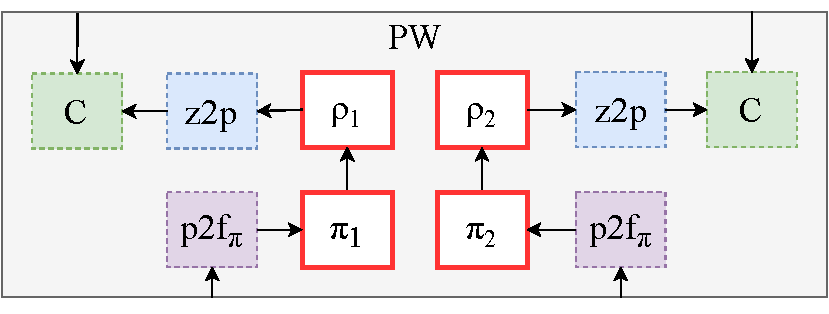
\includegraphics[scale=0.5]{figures/replacement2.pdf}
\caption{When we compose protocols we replace the \emph{p2f} process of $\rho$ with the corresponding instance of $\pi$ and its \emph{p2f} processes. By the emulation theorem, the channel offered by $\rho$ and accepted by $\pi$ have the same type.}
\label{fig:replacement}
\end{figure}

The code for the operator has the same type as any other protocol except, from the description above, it's offered channel is for the type of the functionality $\F_1$ instead of $\F_2$.
We rely on the code generation for to handle spawning instaces of a \inline{p2f} process corresponding to $\pi$ rather than $\rho$.
The operator is given in Figure~\ref{lst:compose}.
\begin{figure}
\begin{lstlisting}[basicstyle=\footnotesize\BeraMonottFamily, frame=single, mathescape]
$\tb{proc}$ compose[K][z,p]:
  (pid: Int), (rng: [Bit]), (sid: session[1]),
  (pid: Int), ($\$$z2p: z) |- ($\$$c: p) =
{
  $\$$ch <- PS.rho <- k rng sid pid $\$$z2p ;
  $\$$c <- Ps.pi <- k rng sid pid $\$$ch 
}
\end{lstlisting}
\caption{The composition operator accepts the same parameters as any other protocol party and offers the channel of type $p2f$ of the realizing protocol $\pi$. We connect $\rho$ to $\pi$ as an environment giving input to $\pi$. We do not need to include any import in our composition operator as the two protocols are guaranteed to be well-matched by the emulation definition. The operator replaces only one party (one \msf{pid}), and the \partywrapper instantiates parties that run the composed protocol.}
\label{lst:compose}
\end{figure}

The resulting composition operator, which composes the two simulators \SIM{\rho} and \SIM{\pi} inside the construction simulator, is best described in text as the resulting code is too verbose to include in the main body of this paper.
You can find the full simulator composition operator in the appendix.
\begin{itemize}
	\item Input from \Z is split between the two simulators
	\begin{itemize} 
		\item \inline{Z2A2P(pid, msg)} intended for parties of $\rho$ are passed to \SIM{\rho}
		\item \inline{Z2A2F(msg)} intended for $\F_1$ is passed to \SIM{\pi}.
	\end{itemize}
	\item Output from \SIM{\pi}: 
	\begin{itemize}
		\item \inline{A2F(msg)} for $\F_2$ and \inline{A2P(pid,msg)} for dummy parties of $\F_2$ are sent to \SIM{\rho} as \inline{Z2A2F(msg)}
		\item \inline{F2A2Z(msg)} is sent to \Z unaltered.
	\end{itemize}
	\item Output from \SIM{\rho}: 
	\begin{itemize}
		\item \inline{A2F(msg)} and \inline{A2P(pid,msg)} for $\F_3$ are sent out unaltered.
		\item \inline{F2A2Z(msg)} messages are sent to \SIM{\pi} as \inline{F2A(msg)} from $\F_2$.
		\item \inline{P2A2Z(pid,msg)} messages are sent to \Z unaltered.
	\end{itemize}
\end{itemize}
The simulator relies on simulators for $\F_1 \xrightarrow{\pi} \F_3$ and $\F_2 \xrightarrow{\rho} \F_3$ to satisfy simulation for Theorem~\ref{thm:singlecomp}.
It is clear that this construction adequately simulates the composed protocol. 
The type in the ideal world gurantees that both the real and ideal world adversaries get at least as much impor as any of the protocol parties. 
This ensures that the composed simulator has enough import to sandbox the two existing simulators and send import out to the ideal world parties and ideal funfctionality.
Therefore it is trivial to see that the composed simulator is well-resource-typed.

Another illustrative description of what composition proposes, logically, is shown by this series of UC executions where the $\equiv$ operator denotes equivalent UC executions that result from moving ITMs in and out of a sandbox, and $\approx$ indicates emulation:
\begin{align}
& \msf{execUC} \: \Z \, (\rho \circ \pi) \, \F_1 \, \DA \\
\equiv \; & \msf{execUC} \: (\Z \circ \rho) \, \pi \, \F_1 \, \DA \\
\approx \; & \msf{execUC} \: (\Z \circ \rho) \, \idealP \, \F_2 \, \SIM{\pi} \\
\equiv \; & \msf{execUC} \: \Z \, \rho \, \F_3 \, (\SIM{\pi} \circ \SIM{\rho})
%\approx \; & \msf{execUC} \: (\Z \circ \Sim{\pi}) \, \idealP \, \F_3 \, \Sim{\rho} \\
%\equiv \; & \msf{execUC} \: \Z \, \idealP \, \F_3 \, (\Sim{\pi} \circ \Sim{\rho}) 
\end{align}

%\item Inputs from \Z of \inline{Z2A2P(msg)} are passed to \SIM{\rho}, and inputs of \inline{Z2A2F(msg)} are passed to \SIM{\pi}.  
%\item \inline{P2A2Z(pid, msg)} outputs from \SIM{\rho} are forwarded to \Z unaltered.
%\item \inline{A2F(msg)} and \inline{A2P(pid, msg)} messages from \SIM{\pi} for $\F_2$ are sent to \SIM{\rho} as \inline{Z2A2F(msg)} and \inline{Z2A2P(pid, msg)}, respectively. 
%\item In the reverse direction, \inline{F2A2Z(msg)} messages from \SIM{\rho} are sent to \SIM{\pi} as \inline{F2A(msg)}, and, finally, \inline{F2A2Z(msg)} output generated by \SIM{\pi} is forwarded to \Z.
%\item \inline{A2P(pid,msg)}, \inline{A2F(msg)} messages from \SIM{\rho}, and \inline{P2A(pid,msg)} and \inline{F2A(msg)} from $\F_3$, are forwarded unaltered. 
%\end{itemize}

%We also provide a composition operator for simulators to construct a simulator for the composed protocol. We connect the simulatorsin the following way
%\begin{figure*}
%\begin{lstlisting}[basicstyle=\small\BeraMonottFamily, frame=single, mathescape]
%$\tb{proc}$ sim_compose[K][a2r,r2a][a2p,p2a][a2f,f2a]:
%  (k: Int), (rnd: [Bit]), (sid: session[1]),
%  (#z_to_a: comm[z2amsg[a2r][a2f]]), (#a_to_z: comm[a2zmsg[r2a,f2a]]),
%  (#a_to_p: comm[a2pmsg[a2r]]), (#p_to_a: comm[p2amsg[r2a]]), (#a_to_f: comm[a2fmsg[a2f]]), (#f_to_a: comm[f2amsg[f2a]])
%    |- ($\$$c: 1) =
%{
%  $\$$ch 
%\end{lstlisting}
%\end{figure*}

%\begin{figure*}
%\begin{lstlisting}[basicstyle=\small\BeraMonottFamily, frame=single,  mathescape]
%$\tb{proc}$ compose[K][z2r][r2z][f2r][r2f][p2f][f2p] : 
%    (pid: Int), ($\$$z_to_p: c[K][z2p]), ($\$$p_to_z: c[K][r2z]), 
%    ($\$$f_to_p: c[K][f2r]), ($\$$p_to_f: c[K][r2f])  |- ($\$$D : 1) =
%{
%	$\$$rho_to_pi <- $\tm{createchan}$[K][p2f];
%	$\$$pi_to_rho <- $\tm{createchan}$[K][f2p];
%
%	 <- pi  <-                 $\$$rho_to_pi $\$$pi_to_rho $\$$p_to_f $\$$f_to_p ;
%	 <- phi <- $\$$z_to_p $\$$p_to_z $\$$rho_to_pi $\$$pi_to_rho ; 
%}
%\end{lstlisting}
%\caption{Composition operator in Nomos that connects a protocol $\rho$ to a protocol $\pi$ that uses some functionality $\F$. The operators creates new channels to connect the realizing $\pi$ and it's hybrid \F. Output from $\rho$ intended for the replace functionality are actually send to parties of $\rho$, and channels outgoing from the parties to the functionality are given to $\pi$.}
%\label{lst:compose} 
%\end{figure*}

%\begin{theorem}[Composition]\label{thm:singlecomp}
%\begin{mathpar}
%\inferrule*[right=single-compose]
%{
%	\F_1 \xrightarrow{\pi} \F_2 \semi \F_2 \xrightarrow{\rho} \F_3 \\
%}
%{
%	\F_1 \xrightarrow{\rho \circ \pi} \F_3
%}
%\end{mathpar}
%
%If \textit{well-typed} $(\pi, \F_1$) realizes $\F_2$ and ($\rho$, $\F_2$) realizes some $\F_3$, then $(\rho \circ \pi, \F_2)$ is \textit{well-typed} and realizes $\F_3$ when $\circ$ is defined as in Figure~\ref{lst:compose}.
%\end{theorem}

%\begin{proof}
%The pre-condition ensures the existence of \textit{well-resource-typed} simulators $\Sim_\rho$ for $\F_2 \xrightarrow{\rho} \F_3$ and $\Sim_\pi$ for $\F_1 \xrightarrow{\pi} \F_2$, and, it is obvious that the composed protocol is also well-resource-typed.
%We construct a simulator \Sim' for the dummy adversary to show
%\[
%	\msf{execUC}\ (\rho \circ \pi)\ \F_1\ \Z\ \A \approx \msf{execUC}\ \idealP\ \F_3\ \Z\ \Sim''
%\]	
%
%The simulator $\Sim'$ relies only simulating \SIM{\pi} and \SIM{\rho}.
%Note that \SIM{\pi} can accept messages for $\pi$ or $\F_1$, simulate them, and generate input for $\F_2$. 
%Similarly, \SIM{\rho} can take inputs for $\rho$ or $\F_2$, simulate them, and generate input for $\F_3$.
%Therefore, we connect the two simulators in the natural way:
%\begin{itemize}
%\item Inputs from \Z of \inline{Z2A2P(msg)} are passed to \SIM{\rho}, and inputs of \inline{Z2A2F(msg)} are passed to \SIM{\pi}.  
%\item \inline{P2A2Z(pid, msg)} outputs from \SIM{\rho} are forwarded to \Z unaltered.
%\item \inline{A2F(msg)} and \inline{A2P(pid, msg)} messages from \SIM{\pi} for $\F_2$ are sent to \SIM{\rho} as \inline{Z2A2F(msg)} and \inline{Z2A2P(pid, msg)}, respectively. 
%\item In the reverse direction, \inline{F2A2Z(msg)} messages from \SIM{\rho} are sent to \SIM{\pi} as \inline{F2A(msg)}, and, finally, \inline{F2A2Z(msg)} output generated by \SIM{\pi} is forwarded to \Z.
%\item \inline{A2P(pid,msg)}, \inline{A2F(msg)} messages from \SIM{\rho}, and \inline{P2A(pid,msg)} and \inline{F2A(msg)} from $\F_3$, are forwarded unaltered. 
%\end{itemize}
%It is clear that \Sim' is able to emulate inputs from \Z to both parties of $\rho$ and the ideal functionalty $\F_1$.
%\Sim' performs constant over head in simulating two \emph{well-resource-typed}, and therefore it is clear that \Sim' is \emph{well-resource-typed}.
%When combined with the \emph{dummy lemma}, a well-resource-typed simulator exists for composition for any adverasry \A. 
%The dummy lemma presented above ensures that a simulator for any \A can be constructed that is well-resource-typed for all wel-resource-typed \A.
%\end{proof}
%
%We give a simpler, high-level idea of the forst step of the proof proof here which can be understood visually:
%The $\equiv$ operator is a result of moving around ITMs (some from within other ITMs into the main UC execution) and $\sim$ refers to indistinguishability.
%In line (13) above, $\rho$ is moved into the execution environment with an unchanged simulator as no additional simulation is required: the simulator allows unfettered communication between parties of $\rho$ and \Z.

\subsection{Multisession}

\begin{theorem}[Composition]\label{thm:composition}
\begin{mathpar}
\inferrule*[right=compose]
{
	%(\pi, !\F_1) \sim (\idealP, F_2) \semi (\rho, !\F_2) \sim (\idealP, \F_3) \\ 
	!\F_1 \xrightarrow{\pi} \F_2 \semi !\F_2 \xrightarrow{\rho} \F_3 \\
	%\Rightarrow \exists \Sim(\A) \vdash (\rho^{!\F_2 \rightarrow (!\pi \, \circ \, \msf{squash})}, !\F_1) \sim (\idealP, \F_3)
}
{
	!\F_1 \xrightarrow{\rho \, \circ !\pi \circ \, \msf{squash}} \F_3
	%(\rho \, \circ \, !\pi \circ \msf{squash}, !\F_1) \sim (\idealP, \F_3)
}
\end{mathpar}
\end{theorem}
Full composition in the UC framework extends beyond the simpler composition in Theorem~\ref{thm:singlecomp} which only defines replacement of one functionality with a protocol that realizes it.
Instead, UC composition allows for replacement of any number of instances of a functionality with instancesof the realizing protocol.
Theorem~\ref{thm:composition} illustrates the full composition theorem using our arrow notation, and highlights a theorem that we must prove before we can achieve full composition.
It relies on Theorem~\ref{thm:squash} that introduces the \msf{squash} protocol and the $!$ operator.
Notice that Theorem~\ref{thm:compose} follows directly from Theorem~\ref{thm:singlecomp} and Theorem~\ref{thm:squash}.

The multi-session extension of a protocol or functionality, specified by the $!$ operator (such as $!\rho$ or $!\F$), allows multiple instances of the protocol/functionality to be run within a sinlge ITM.
An ITM simulates the instances and multiplexes input/output to/from them much like the \partywrapper.

\begin{theorem}[Squash Theorem]\label{thm:squash}
%If a functionality \F is well-resource-typed, then $!\F$ and $!!\F$ are well-resource-typed (by Theorem~\ref{thm:bangppt}) and $(\idealP, !!\F) \sim (\msf{squash}, !\F)$.
%\textit{Well-resource-typed} \F $\Rightarrow$ $!\F \xrightarrow{\msf{squash}} !!\F$%  $(\idealP, !!\F) \sim (\msf{squash}, !\F)$
\begin{mathpar}
\inferrule*[right=squash]
{
\textit{well-resource-typed} \; \F
}
{
!\F \xrightarrow{\msf{squash}} !!\F
}
\end{mathpar}
\end{theorem}

For the multisession extension of a fuctionality, the type is straightforward and ony acts to multiplex input/outpt based on the intended target \inline{ssid}.
\begin{center}
\parbox{0cm}{
\begin{tabbing}
$\m{{P2MS}[a,b]\{n,m\}} = \textcolor{red}{\getpot^n} \ichoice{\mb{Inp}: ssid \arrow a \tensor \echoice{$\=$\mb{Ok}: \textcolor{red}{\paypot^0} \; \m{P2MS[a,b]\{n,m\}},$ \\
\>$\mb{Out}: ssid \arrow b \tensor \textcolor{red}{\paypot^m} \; \m{P2MS[a,b]\{m,n\}}}}$
%\m{MS2P[a][b]\{n,m\}}}$ \\
%\mi{stype} \; \m{{MS2P}[a][b]\{n,m\}} = \echoice{\mb{Ok}: \textcolor{red}{\paypot^0} \; \m{P2MS[a][b]\{n,m\}}, \mb{Out}: ssid \product b \arrow \textcolor{red}{\paypot^m} \; \m{P2MS[a][b]\{n,m\}}}  
\end{tabbing}}
\end{center}
The multisession extension is mentioned in greater detail in the appendix.
%and the functional types that are sent to the wrapper surrounding it are given by
%\begin{lstlisting}[basicstyle=\small\BeraMonottFamily, mathescape]
%$\yo{type}$ p2ms[a] = P2MS of ssid ^ a ;
%$\yo{type}$ ms2p[b] = MS2P of ssid ^ b ;
%\end{lstlisting}
%It is important to note that we require a session type here instead of allowing !\F act as the functionality wrapper because, when composed it must communicate directly communicate, over a session-typed channel, to another protocol.
%Furthermore, the construction of !\F is the same as in the \Fro example: one session typed channel for all parties.
%In Figure~\ref{fig:multisession} illustrated the functionality wrapper (right) and the multisession extension (left) for \Fcom. 
%\begin{figure}
%\centering
%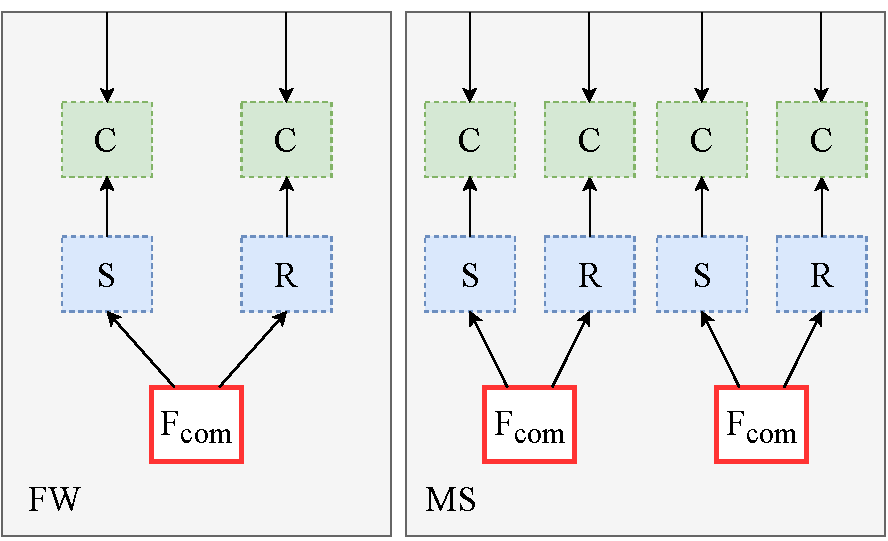
\includegraphics[scale=0.5]{figures/multisession.pdf}
%\caption{The multisession extension of \Fcom (right) with only two instances, creates the same processes $S$ and $R$ (offering the session typed channel to \Fcom) for every created instance. A communicator per session buffers messages for the $S$ and $R$ processes to consume and forward along their session-typed channel to \Fcom.}
%\label{fig:multisession}
%\end{figure}

%As a generic construction provided by NomosUC, the multisession operator requires some code generation but only to accept an arbitrary number of virtual token types if the underlying \F simulators other processes. 
%Furthermore, similar to the functionality wrapper, the multisession operator constructs the processes around \F in the same way and spawns them on-demand.
%The process definition for $!\F_\msf{com}$ is shown in Figure \ref{lst:bangf} accepting two token types: the real token type $K$ and the virtual token type $K_1$ for instances of $\F_\msf{com}$.
%
%\begin{figure}
%\begin{lstlisting}[basicstyle=\footnotesize\BeraMonottFamily, frame=single, mathescape]
%$\tb{proc}$ bangF[K,K1][p2f,...] :
%  (k: $\tgr{Int}$), (rng: [Bit]), (sid: session[a]), 
%  ($\$$p: P2MS[p2f][f2p]) |- ($\$$ch: 1) =
%\end{lstlisting}
%\caption{The type definition for the multisession operator for functionalities and the correspond message type and import parameters. The operator for protocol parties is identical in code but differens in that the parameters to the \texttt{P2MS} type are for \texttt{Z2P} interaction.}
%\label{lst:bangf}
%\end{figure}

\begin{theorem}[PPT !]\label{thm:bangppt}
If a functionality $\F$ is well-resource-typed, then it's multisession extension $!\F$ is well-resource-typed.
\end{theorem}

We examine this theorem in greater detail in the appendix. 
At a high-level it is obvious that such a construction, activated polynomially many times, is well-resource-typed as long as the underlying functionality/protocol is well-resource-typed.
%\begin{proof}
%A \textit{well-resource-typed} \F guarantees a polynomial $T_{\F}$ bounding its execution.
%In the worse-case, the multisession operator must spawn a new instance of $\F$ an every activation. 
%Let $N_{\F}$ denote the total number of instances (and, hence, number of activations) of $\F$ created by the operator.
%Note that $N_{\F}$ is polynomial in the security parameter $k$ for all well-typed environments, protocols, and adversary.
%Therefore, there always exists a bounding polynomial to bound a polynomial number of simulated instances of \F.
%The polynomial can be given as:
%$$ P_{!\F}(n) = N_{\F} P_{\F}(n) + \mathcal{O}(N_{\F}) $$
%where the $\mathcal{O}(N_{\F})$ is due to the overhead of maintaining and accessing the set of all instances.
%
%Similarly, \F being \textit{well-resource-typed} ensures a valid token context for all processes it may simulate. 
%Therefore, it is clear that there exists a global connecting poltnomial $f$ that ensures a valid token context for $!\F$.
%\end{proof}


%\begin{figure}
%\begin{lstlisting}[basicstyle=\small\BeraMonottFamily, mathescape, frame=single]
%$\yo{type}$ p2bFmsg[a] = P2bF of ssid ^ a ;
%$\yo{type}$ p2bbFmsg[a] = P2bbF of ssid ^ ssid ^ a ;
%$\tg{(* z2p : comm[z2pmsg[p2bbf[a]]] *)}$
%$\tg{(* p2f : comm[p2fmsg[P2bf[a]]] *)}$
%pid = recv $\$$z2p ;
%m = recv $\$$z2p ;
%case m (
%  P2bbF(ssid1, ssid2, m) =>
%    send $\$$p2f P2bF(ssid1 + ssid2, m) ;
%)
%\end{lstlisting}
%\caption{The \textit{squash protocol} accepts a message intended intended for $!!\F$ of type \inline{P2MS[p2ms[a]][ms2p[b]]}, i.e. of the form $(\msf{ssid}_1, (\msf{ssid}_1, msg))$.
%It ``flattens'' it into a single $\msf{ssid}_3 = \msf{ssid}_1 + \msf{ssid}_2$ that can be passed to $!\F$. The result is the same number of instances of \F but behind only a single $!$ operator.}
%\label{fig:squash}
%\end{figure}

\begin{proof} (Theorem~\ref{thm:squash})
On examination the \msf{squash} theorem does constant work per activation and concantenates two \inline{ssid}s into one for messages going to the functionality and does the inverse for messages incoming from the functionality.
We provide more detail for a proof of Theorem~\ref{thm:squash} in the Appendix, however, it is clear to see that the this theorem holds with a trivial simulator.
%First we describe the \msf{squash} protocol where $!!\F$ are nested $!$ operators.
%The protocol accepts messages intended for $!!\F$ of type \inline{P2MS[p2ms[a]][ms2p[b]]}, i.e. of the form $(\msf{ssid}_1, (\msf{ssid}_2, msg))$, and ``flattens'' them into a single message of type $\inline{P2MS[a][b]}$, i.e. of the form $(\msf{ssid}_3, msg)$.
%
%In $(\idealP, !!\F)$, \idealP~expects to receive messages of the form $(\msf{ssid}_1, (\msf{ssid}_2, m))$ where $\msf{ssid_2}$ is a sub-session of $\F$ (i.e. instance) inside some $!\F$ with sub-session id $\msf{ssid}_1$ inside of $!!\F$ (the message accesses functionality $\F[\msf{ssid}_1][\msf{ssid}_2]$).
%The \msf{squash} protocol flattens the indexing of instances of \F and combines session ids $\msf{ssid}_1$ and $\msf{ssid}_2$ into a single \msf{ssid}: $\msf{ssid}_3 := \msf{ssid}_1 \cdot \msf{ssid}_2$.
%If follows intuitively that the view for the environment remains the same. 
%
%We construct a simulator such that:
%\[
%\msf{execUC} \, \Z \, \idealP \, !!\F \, \SIM{\msf{squash}} \approx \msf{execUC} \, \Z \, \msf{squash} \, !\F \DA 
%\]
%The simulator is very simple. 
%Inputs to/from parties/\Z for a corrupt party is forwarded unmodified.
%Input intended for $!\F$ of the form $(\msf{ssid}_1 \cdot \msf{ssid}_2, msg)$ is sent as $(\msf{ssid}_1, (\msf{ssid}_2, msg))$ to $!!\F$. 
%Output from $!!\F$ is modified inversely and sent to \Z.
%
%The proposed simulator is trivially analyzed to be \textit{well-resource-typed}.
%It performs constant work per activation and does ``real'' simulation other than message modification to/from $!!\F$.
\end{proof}

\subsection{UC Composition}
Finally, we can conlude with full composition in Theorem~\ref{thm:compose}.
The proof follows directly from Theorems~\ref{thm:singlecomp} and \ref{thm:squash}.

\begin{proof}
By Theorem~\ref{thm:singlecomp} we can construct a simulator \SIM{1} for $!!\F_1 \xrightarrow{\rho \, \circ \, !\pi} \F_3$.
Theorem~\ref{thm:squash} then allows us to ``squash'' $!!\F_1$ and construct a simulator using \SIM{1} for $!\F_1 \xrightarrow{\rho \, \circ \, !\pi \, \circ \, \msf{squash}} \F_3$
\end{proof}

\subsection{Design Discussion}
One of the core research questions that this work aims to study session types applied to the UC framework. 
In this section, we discuss how resource-aware session types impact the design of functionalities in NomosUC as well as which are implementable.
We use the two-way authenticated channel functionality \Fauth to througout this discussion.

In plain session types, communication between two parties $P_s$ and $P_r$ occurs over a single duplex channel.
In UC the role of the adversary as a message scheduler in \Fauth, the most common network channel model, means a more complicated functionaty involving $P_s$, $P_r$, \F, and \A. 
The simplest, and most common approach, to \Fauth is the following communication pattern: a party $P_s$ sends a message to \Fauth, \Fauth sends the message to \A and waits for \A to say \inline{OK} before delivering the message to $P_r$.
Since both parties can send a message and receive a message, it is unclear which process, \Fauth or $P$, will be active along that channel at any given time.
Session types require this information to be statically known when two processes are communicating over a single channel--making this communication pattern unexpressable over a single channel.

There a few ways to overcome this constraint. 
In general, even though the UC framework places few restructions of communication patterns, most functionalities stick to a few.
\Fauth, for example, can take a few forms:
\begin{enumerate}
\item (presented above) Receiver and adverasry are activated directly: \Fauth waits for \A to tell it to deliver the message.
\item \Fauth ``polling'' approach: messages from $P_s$ are buffered for both \A and $P_r$. \A and $P_r$ must ask \Fauth for new messages. This is a more invonconvenient method, but can be useful for novel functionality designs that need a channel.
\item ``polling'' but receiver is activated: the message is stored in a buffer for \A, and \A's deliver message directly sends it to $P_r$.
\end{enumerate}
The simplest way to implement \Fauth in NomosUC is ``polling'' approach. As far as we know, we can systematically tranform any UC functionality into one that uses ``polling''. 
The consequences are that polling is inconvenient from a programming point of view because \Z needs to continuously activate parties to ask for new messages.
Hope is not lost though, because it turns out our type system can express functionalities in all three of the ways listed above. 
The first, and most natural, approach only requires splitting communicating between $P$ and \Fauth into two unidirectional channels
Such an extension to NomosUC trivially modifies the \partywrapper to handle two channels instead of one, and the types of the channels can be succintly expressed as: 
\begin{center}
\parbox{0cm}{
\begin{tabbing}
$\m{sending}[a] = \textcolor{red}{\getpot^n} \ichoice{\mb{sendmsg}: \m{a} \tensor \m{sendmsg}}$ \\
$\m{receive}[a] = \textcolor{red}{\getpot^m} \echoice{\mb{recv}: \m{a} \tensor \m{receive}}$ \\
$\m{adv}[a] = \echoice{\mb{leakmsg}: a \tensor \ichoice{ \mb{ok}: \m{leakmsg}}}$
\end{tabbing}}
\end{center}
The first to correspond to the channels for sending from $P$ to \Fauth and the second in the opposite direction. The third is the adversary's channel at \Fauth.

A notable part of our contruction is the machinery created around the protocol parties and functionality that intemediate their communication with communicators and functionally-typed messages.
Recall that such compromises are required in order to allow a \emph{dynamic} number of parties in UC.
The session type of the shared channel of a communicator only allows for a fixed amount of import to be sent over it with every messages. 
Protocols and functionalities that send different amounts of import depending on the message, say $i_1,...,i_n$, must now send $\m{max}(\{i_j\})$ import with every messages.
For existing UC definitions this appears to be an issue of ensuring a machine has \emph{enough} import, however, we can systematically map any UC import definition to one that works in NomosUC~\footnote{The problem can be reduced to ensuring enough ``latent'' import needed to compute, and, because we aren't concerned here with \emph{tight} computational bounds the problem is quite easy to solve. We discuss in greater detail in the appendix.}.



%\caption{The \msf{execUC} function used for the two-party commitment example used throughout this paper. Recall, the \msf{execUC} is customized insofar as it takes in some number of virtual token types (here, $K_1$) to enable machines that simulate other machines. In the commitment example, there is no such simulation happening at the protocol or functionality level, therefore only the real token type $K_1$ is used here. The funtion spawns all the necessary ITMs in the UC execution: the environment, the protocol wrapper, the functionalty (wrapped), and the adversary. Each is parameterized with the security parameter $k$ and a random bit sequence $\msf{rng} \in \{0,1\}^{poly(k)}$.
%At the end, the environment is started and it returns a bit $b$ which is its guess for which world it is in. The full code can be found in the Appendix.}
%\label{lst:execuc}
%\end{figure*}

%Communication between all of the major processes in the UC execution (\Z, \A, \partywrapper, and \fwrapper) is done through communicators introduced in Section~\ref{sec:nomosuc}.
%Communicators are restricted to only sending functionally types messages in NomosUC, and we give generic types, below, to all such messages.
%\todo{Is this important to even have here? seems a useless implementation detail.}
%\begin{lstlisting}[basicstyle=\footnotesize\BeraMonottFamily, frame=single, mathescape]
%$\Type$ p2zmsg[a] = P2Z of pid ^ a ;
%$\Type$ p2fmsg[a] = P2F of pid ^ a ;
%$\Type$ f2pmsg[a] = F2P of pid ^ a ;
%\end{lstlisting}

\paragraph{The Environment}
The environment is the first machine that \inline{execUC} spawns and receives from it the session id and list of corrupted parties for this execution. 
It can be considered the \emph{first} ITM in the execution.
Its role in the execution is specified by the type \inline{EtoZ} of the channel it offers.
\begin{lstlisting}[basicstyle=\footnotesize\BeraMonottFamily, mathescape, frame=single]
$\Type$ EtoZ[a] = +{init: a ^ list[pid] -> exec} 
$\Type$ exec = &{start : output_bit} ;
$\Type$ output_bit = +{bit: Bit -> 1} ;

$\tb{proc}$ PS.env[K][z2p,...]{p2zn,...} : 
  (k: $\tgr{int}$), (r: [Bit]), (#ztop: comm[z2pmsg[z2p]]{z2pn}), 
  (#ptoz: comm[p2zmsg[p2z]]{p2zn})...  |- ($\$$z : EtoZ) $\tg{(* <- offered channel *)}$
\end{lstlisting}
It reflects that the environment must first determine the session id, or \inline{sid}, of the execution as well as which parties it wants to statically corrupt in the form of a \inline{list} of \inline{pid}s.
Finally, it is told to start and eventually returns an output \inline{bit} indicating it's guess as to whether it's in the real world or the ideal world.
This output bit, and the environment's decision function, go on to define emulation and indistinguishability later in this section. 

%The environment also accepts communicators, as parameters, for communication with the protocol parties and the adversaries (in both directions), and offer a channel \inline{$\$$z} of type \inline{EtoZ}.
%The type (above) states \Z provides an \emph{sid} of some user-defined type \inline{a} and a list of the \emph{pid}s of corrupted parties. 
%Finally, \inline{execUC} instructs it to \inline{start} (\emph{external choice}) and return a bit $b$ as its guess for which world it is in.

%The communicators created by \inline{execUC} always use the same parametric types. 
%For example, for communication with the protocol, the types look like:
%\begin{lstlisting}[basicstyle=\small\BeraMonottFamily, frame=single, mathescape]
%$\Type$ p2zmsg[a] = P2Z of pid ^ a ;
%$\Type$ p2fmsg[a] = P2F of pid ^ a ;
%$\Type$ f2pmsg[a] = F2P of pid ^ a ;
%\end{lstlisting}
%Subsequently, the channel from \Z to the protocol wrapper will be typed as: \inline{comm[z2pmsg[z2p]]\{z2pn\}} where \inline{z2p} is a protocol-specific message type.
%The protocol \inline{PS.prot} is not spawned by \inline{execUC}. Instead the process spawns the protocol wrapper (described below) which spawns parties with that run the code \inline{PS.prot}.
%When in the ideal world, the protocol is given as the ideal protocol: one where the protocol wrapper converts the message from type \inline{z2pmsg[a]} to type \inline{p2fmsg[a]} but forwards the contents unaltered.
%The protocol wrapper and functionality wrapper manage spawning the instance(s) of the functionality and protocol parties.
%Similarly, an environment \msf{PS.env} and adversary \msf{PS.adv} must be defined as well.
%The message types exchanged between the processes are provided directly to \msf{execUC} as type parameters of the form \msf{p2f}, \msf{f2p}, and so on. 
%The first thing \inline{execUC} does is create the communicators and the corresponding channels for the main processes of the execution. 

%A consequence of using communicators is that in the UC setting they require at least 1 unit of import, beacuse they are activated a potentially polynomial number of times. 
%Therefore, all communicators in NomosUC receive some amount of import $n$ and send out only $n-1$. 
%The user-specified protocol, environment, functionality, and adverasary must account for this to ensure suffiient import is given to them.
%\begin{lstlisting}[basicstyle=\small\BeraMonottFamily, frame=single, mathescape]
%#ptoz <- communicator_init[K][p2zmsg[p2z]]
%           {p2zn+1} ;
%#ztop <- communicator_init[K][z2pmsg[z2p]]
%           {z2pn+1} ;
%...
%\end{lstlisting}
%This is strictly a design decision where user-defined protocols only specify import token requirements for the protocol not taking communicators into account. 
%The processes that they write, though, must conform to this standard and send an import token in addition to the amount they need.
%An alternate design would be that all import type parameters take the additional import token into account and communicators send one less than they receive.
%The drawback of the latter approach is that that when communicating with a process directly rather than through communicators (say, when simulating), you're sending one extra token for no reason.

%Next, the environment \msf{PS.env} is spawned, \inline{execUC} receives the \inline{sid} and corrupt list from \Z, and, finally, the remainder of the processes are spawned with these inputs. 
%Finally, the environment executes its own code when activated by \msf{\$z.start}, given the initial amoutn of import \inline{n}, and returns a bit through \inline{$\$$z.output_bit} which is its guess whether it's in the real or ideal world:
%\begin{lstlisting}[basicstyle=\small\BeraMonottFamily, frame=single, mathescape]
%$\$$z.start
%$\tb{pay}$ $\$$z {n}
%$\$$d <- $\$$z
%\end{lstlisting}

\subsection{Ideal Functionalities}
One of the core research questions that this work aims to study session types applied to the UC framework. 
In this section, we discuss how resource-aware session types impact the design of functionalities in NomosUC.
We use the two-way authenticated channel functionality \Fauth to throughout this discussion.

In plain session types, communication between two parties $P_s$ and $P_r$ occurs over a single duplex channel.
In UC the role of the adversary as a message scheduler in \Fauth, the most common network channel model, means a more complicated functionality involving $P_s$, $P_r$, \F, and \A. 
The simplest, and most common approach, to \Fauth is the following communication pattern: a party $P_s$ sends a message to \Fauth, and \Fauth sends the message to \A and waits for \A to say \inline{OK} before delivering the message to $P_r$.
Since both parties can send and receive messages, it is unclear which process, \Fauth or $P$, will be active along their mutual channel at any given time.
Session types require this information to be statically known when two processes are communicating over a single channel--making this communication pattern unexpressable over a single channel.

There a few ways to overcome this constraint. 
In general, even though the UC framework places few restrictions of communication patterns, most functionalities stick to a few.
Despite the constraint above, our type system is able to express each of the following implementations of \Fauth:
\begin{enumerate}
\item (presented above) Receiver and adversary are activated directly: \Fauth waits for \A to tell it to deliver the message. If we extend the parties and functionality to communicate over two unidirectional channels. Given the type
\begin{center}
\parbox{0cm}{
\begin{tabbing}
$\m{sending}[a] = \textcolor{red}{\getpot^n} \ichoice{\mb{sendmsg}: \m{a} \tensor \m{sendmsg}}$ \\
$\m{receive}[a] = \textcolor{red}{\getpot^m} \echoice{\mb{recv}: \m{a} \tensor \m{receive}}$ \\
$\m{adv}[a] = \echoice{\mb{leakmsg}: a \tensor \ichoice{ \mb{ok}: \m{leakmsg}}}$
\end{tabbing}}
\end{center}
mitigates the problem.
The first two correspond to the channels for sending from $P$ to \Fauth and the second in the opposite direction. The third is the adversary's channel at \Fauth.
\item \Fauth ``polling'' approach: messages from $P_s$ are buffered for both \A and $P_r$. \A and $P_r$ must ask \Fauth for new messages. This is more inconvenient from the point of view of simplicity of the code, however, it is a common approach used given its flexibility and only requires a single channel in here. It's type can be given as
\begin{center}
\parbox{0cm}{
\begin{tabbing}
$\m{receive}[a] = \textcolor{red}{\getpot^m} \ichoice{\mb{recv}: \echoice{$\=$\mb{yes}: a \tensor \m{receive}[a] $ \\
\>$\mb{no}: \m{receive}[a]}}$ \\
$\m{adv}[a] = \ichoice{\m{get}: \echoice{$\=$\mb{yes}: a \tensor \m{adv}[a]$ \\
\>$\mb{no}: \m{adv}[a]}}$
\end{tabbing}}
\end{center}
\item ``polling'' but receiver is activated: the message is stored in a buffer for \A, and \A's deliver message directly sends it to $P_r$. This approach, like the first, requires two uni-directional channels. The type of this approach is the same as $\m{sending}[a]$/$\m{receive}[a]$ from the first bullet and $\m{adv}[a]$ from the second one.
\end{enumerate}

%Recall that such compromises are required in order to allow a \emph{dynamic} number of parties in UC.
%The session type of the shared channel of a communicator only allows for a fixed amount of import to be sent over it with every messages. 
%Protocols and functionalities that send different amounts of import depending on the message, say $i_1,...,i_n$, must now send $\m{max}(\{i_j\})$ import with every messages.
%For existing UC definitions this appears to be an issue of ensuring a machine has \emph{enough} import, however, we can systematically map any UC import definition to one that works in NomosUC~\footnote{The problem can be reduced to ensuring enough ``latent'' import needed to compute, and, because we aren't concerned here with \emph{tight} computational bounds the problem is quite easy to solve. We discuss in greater detail in the appendix.}.


\subsection{The \partywrapper}
NomosUC departs slightly from the standard UC framework by using a \partywrapper to encapsulate all protocol parties and run them internally, and using communicators to intermediate communication between \Z, \A, \F, and the \partywrapper.
We use the notation \m{PW}(\PI) to denote the party wrapper running parties of protocol \PI.

The purpose of the wrapper is to support a dynamic set of parties without \Z, \A, or \F having to reat to new parties and managing a growing set of channels.
Instead, the \partywrapper acts as singular endpoint for all communication with protoco parties, and it manages the creation of new parties and routing messages to/from them.

From the point of view of parties running inside the \partywrapper, they are directly connected to \F and \Z in the way of Figure~\ref{fig:newpandq}.
The shell code offers four channels, two from \F and two from \Z, that offer the appropriate session types. 
For commitment, the processes for \Z offer channels with type \m{sender} or \m{receiver}, and processes for \F offer the type of the hybrid functionality \Fro which we examine later.
However, because we run parties of \PI internal to the \partywrapper, it runs instances of the shell code for each new spawned party and created communicators around it that it can write/read pid-specific messages to/from.
Figure~\ref{fig:singlemultiplex} illustrates how the shell code $\pi_{pid}$ is connected to communicators for each direction. This construction is repeated for every new paty spawned inside the \partywrapper.

%\paragraph{Communicators}
%One consequence of the \partywrapper and our construction of the UC experiment is that we intermediate communcation between the major processes in NomosUC, with communicators.
%For example, if we opt for a linear channel, offered by the party wrapper or \Z, for communication between between them, then its type must be static and therefore can no longer handle an arbitrary number of parties.
%Similarly, a channel offered by
%One consequence of the \partywrapper is that communication in the UC experiment is intermediated by communicators in NomosUC.
%The singular endpoint for all party communications makes it difficult to connect \pw directly to \Z with a session typed channel.
%Session types are statically typed, therefore, it is not possible to modify the session type of a single channel to accomocate newly created parties with potentially differing types. 
%Communicators enable NomosUC to continue using session types to govern communication between \Z, \PI, and \F by intermediating communication with functional messages.
%The \pw runs the protocol parties internally with their session types, and shuttles incoming functionally typed messages to those channels and vice versa for outgoing messages.
%
%Figure~\ref{fig:blankpartywrapper} shows the internals of \pw for two parties. The process \inline{C} demultiplexes incoming messages based on \inline{pid}, and the \inline{z2p} and \inline{f2p} processes convert to/from functionally typed messages. 
%
%Obviously, the processes \inline{z2p} and \inline{f2p} are protocol/functionality specific.
%Therefore, like \iexecuc, we generate those processes for the \partywrapper based on the protocol/functionality definition provided by the user~\footnote{It is equally valid to not generate them but let the user write the code for them manually. However, given the straightfoward nature of the processes, we opt to relieve the user of this burden.}.
%
%We provide an example of what \inline{z2p} does for a commitment protocol when the \partywrapper receives messages typed as:
%\begin{lstlisting}[basicstyle=\footnotesize\BeraMonottFamily, mathescape]
%$\yo{type}$ comp2f = Commit of Bit | Open ;
%$\yo{type}$ comf2p = Committed | Open of Bit ;
%\end{lstlisting}
%\inline{z2p} intercepts receives the message and communicates the message to the committer over its channel:
%\begin{lstlisting}[basicstyle=\footnotesize\BeraMonottFamily, frame=single, mathescape]
%case msg (
%  Commit(b) =>
%    $\$$z2p.commit ;
%    $\tb{send}$ $\$$z2p b ;
%    $\tb{pay}$ {z2pn} $\$$z2p ;
%\end{lstlisting}
%Here \inline{z2p} in the code refers to the committer's channel for \Z
%The \inline{f2p} processes does the same for communication between the parties and the functionality.
%
%As a resut of their session types, communicators also require that all messages be sent with some static amount of import.
%Therefore, a user must set import requirements for a protocol work in this constrainted system.
%Furthermore, as far as we know, we can systematically map any UC import definition to one that works in NomosUC.

\paragraph{Import with the \partywrapper}
Virtualizing protocol parties in a wrpper means that they all, effectively, share the same \emph{real} import and potential, even though they are given virtual potential.
We reason that the \partywrapper does not change the import requirements of protocols or make some protocols unrealizable in NomosUC.
Mainly, for any activation of a party, the party either retains some import or gives away all the import it receives. 
The former case allows parties to do polynomial work or be activated a polynomial number of times, and the latter case allows for parties activated a constant number of times and doing constant work per activation.
The \partywrapper alone does constant work per activation, therefore, in either case boththe protocol party and \partywrapper have enough import to perform their necessary computations.

\begin{figure}
	\centering
	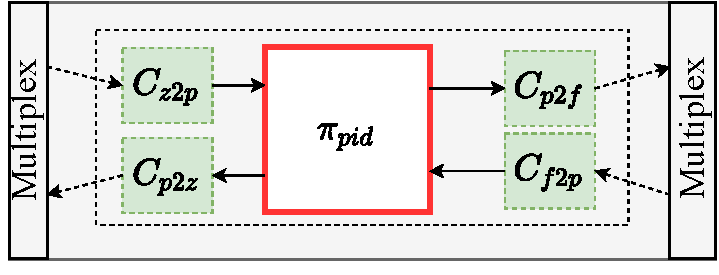
\includegraphics[scale=0.5]{figures/singleshellmultiplex.pdf}
	\caption{An instance of a single protocol party. The party $\pi_{pid}$ is the shell code around the actual protocol akin to Figure~\ref{fig:newpandq}, and it is given communicators for communication in both directions. The dotted box encapsulates all the code that the \partywrapper creates for each party.}
	\label{fig:singlemultiplex}
	\vspace{-3mm}
\end{figure}


%\begin{figure}
%\centering
%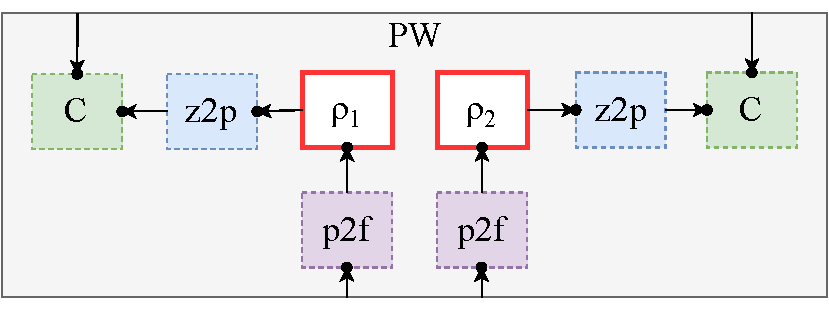
\includegraphics[scale=0.5]{figures/blankpartywrapper2.pdf}
%\caption{The internals of the protocol wrapper with two parties. The arrows indicates the client/provider relationship between each pair: provider $\rightarrow$ client. The wrapper creates \texttt{z2p} to offer a channel and convert from gunctional to message type---the \texttt{p2f} do the same. A communicator is used because \texttt{z2p} cannot send message to real one with differing token type. The types of the processes offered are (color): \tgr{comm[z2pmsg[comp2f]]}, \tb{sender}, \tr{party[Int]}, \tp{comm[p2fmsg[rop2f]]}. }
%\label{fig:blankpartywrapper}
%\vspace{-1.5em}
%\end{figure}

%For the commitment example, if $\pi_1$ and $\pi_2$ ran the commitment protocol, \inline{z2p} would offer a channel of type \inline{sender} and \inline{receiver} to $\pi_1$ and $\pi_2$, respectively, and it converts between the functional messages for the commitment protocol and the session typed ones. 
%In the ideal world, the $\pi_1$ and $\pi_2$ run a dummy protocol where their offered channels are simply forwarded to their \inline{z2p} channels, i.e. the \inline{z2p} and \inline{f2p} channels have the same type: \inline{sender} and \inline{receiver}, respectively.
%In the style of Nomos, the protocol wrapper:
%\begin{itemize}
%	\item Attempts to read messages incoming from \Z, \A, or \F and forward them to the appropriate process depending on \inline{pid}.
%	\item Read from the internal communicators or the \inline{p2f} processes for outcoing messages.
%\end{itemize}
%For reference the functional messages typed for the commitment protocol are:

%Recall the session types for the sender and receiver, with \Fcom, introduced in Section \ref{subsec:idealcommitment}.
%%\begin{gather}
%%	\mi{stype} \; \m{sender} = \ichoice{\mb{commit} : \m{bit} \product \m{scommitted}} \\
%%	\mi{stype} \; \m{scommitted} = \ichoice{\mb{open} : 1} \\
%%	\mi{stype} \; \m{receiver} = \echoice{\mb{commit} : \m{rcommitted}} \\
%%	\mi{stype} \; \m{rcommitted} = \echoice{\mb{open} : \m{bit} \arrow \one}
%%\end{gather}
%At the beginning there are no parties. When the \A or \Z write to a party with some pid $p$ the protocol wrapper creates $p$ if it does not exist.
%It creates and stores the session-typed channels or all of the parties in channels corresponding to their type and moves channels between them as the type evolves.
%For example for parties' channel with \Z the protocol wrapper generates the following lists:
%\begin{gather}
%	\m{R1L1}[\m{sender}] \\
%	\m{R1L2}[\m{scommitted}] \\
%	\m{R2L1}[\m{receiver}] \\
%	\m{R2L2}[\m{rcommitted}] 
%\end{gather}
%At the beginning of the protocol, the committer's \msf{z2p} channel would be in \inline{R1L1} and the receiver's is in \inline{R2L1}.
%The channel's connection the protocol wrapper to the rest are still functionally typed. It's channel \inline{p2f} will still be typed \inline{#ptof: comm[p2fmsg[comp2f]]} where \inline{comp2f} is:
%Succinctly, the protocol wrapper functions as follows:
%\begin{itemize}
%\item When the protocol wrapper receives a message for some \msf{pid}, if the party doesn't exist the protocol wrapper creates all the party's channel parameterized by the correct session types (the role of the party is determined by the incoming message). The channels are stored and outgoing channels are waiting to be read from.
%\item The message sent to the party with the session type is determined by the functional type. The wrapper creates a session-typed message and forwards the contents of the message to the party.
%Despite accepting functionally typed messages, the protocol wrapper uses session types in this way to allow the type checker to catch invalid and out of order environments, adversaries and functionalities. 
%For example, in the commitment protocol when the committer tries to commit a bit in \Fcom like this:
%\begin{lstlisting}[basicstyle=\small\BeraMonottFamily, frame=single, mathescape]
%$\$$p2f.commit 
%$\tb{send}$ $\$$p2f b
%$\tb{pay}$ {p2fn} $\$$p2f
%\end{lstlisting}
%\begin{lstlisting}[basicstyle=\small\BeraMonottFamily, frame=single, mathescape]
%$\$$p2f.SEND 
%$\tb{send}$ $\$$p2f pid 
%$\tb{send}$ $\$$p2f Commit(b)
%$\tb{pay}$ {p2fn} $\$$p2f
%\end{lstlisting}
%The party wrapper intercepts and converts it to a functionally typed message:
%\item For outgoing messages, the protocol wrapper does a similar conversion where it reads the sesion typed channel output by the party and converts its message to the appropriate functional message type.
%\end{itemize}

%\paragraph{Functionality Wrapper}
%The \fwrapper adopts a similar approach to the \partywrapper, except it only creates one instance of the underlying functionality.
%For the same reason as the \partywrapper, we use an \fwrapper to enable a dynamic set of parties.
%One caveat in supporting such functionalities, is that, so far, only functionalities whose type follows a specific form are allowed.
%In the random oracle type given below, notice that the type before and after a party interacts with it is the same: type $\m{party}[a]$.
%\begin{mathpar}
%\m{party}[a] = \textcolor{red}{\getpot^1} \ichoice{\mb{hash} : \m{pid} \arrow \m{int} \product \m{hashing}[a]} \\
%\m{hashing}[a] = \echoice{\mb{shash} : \m{pid} \arrow \m{int} \product \textcolor{red}{\paypot^0} \m{party}[a]} 
%\end{mathpar}
%A party queries a $\mb{hash}$ of an integer from \Fro and receives an integer as a response. The session type includes the \inline{pid}, which enables it to handle all parties over the same channel.
%
%An example of the internals of the \fwrapper are showing on the left-hand-side of Figure~\ref{fig:multisession}.
%Like the \inline{z2p} processes in the \partywrapper, \inline{S} and \inline{R} represent the sender and receiver in the commitment protocol, and they read from their virtual communicators and communicate with \Fcom over a session-typed channel.

%When a party invokes \Fro, the type it expects is \inline{party[a]}, and when it has received its hash the type is again back at \inline{party[a]}. 
%The wrapper handles such dynamic functionalities by channeling all party communication through one linear channel in the wrapper. 
%Therefore, \Fro reads on one channel and responds to the specific party with some \inline{pid}, and the protocol wrapper remains unchanged. 
%
%The constructions of the protocol wrapper and functionality wrapper enable users to write very simple ideal functionality and protocol code, as we will discuss in the next Section and in the Appedix.

%In the commitment example, \Fcom accepts two channels, one from each party, and two processes are created (call then \inline{p2f} for now) which offer channels of type \inline{sender} and \inline{receiver}, respectively. 
%The wrapper differs from the protocol wrapper for certain functionalities that accept a dynamic number of parties. 
%Continuing with our commitment example, the random oracle functionality, an idealized hash function, is used in the real world to realize \Fcom, and it allows a dynamic set of parties to inteact with it.
%Its session type with protocol parties is given below.
%The session type is special in that, for every interaction, the channels type always ends up back at \inline{party[a]} before any other party tries to use \Fro.
%NomosUC enables ideal functionalities whose types work like this by adding the \inline{pid} to the type, and having only one process in the functionality wrapper offering a channel of this type to \Fro.
%Unlike \Fcom where new communicator and \inline{p2f} process is created for each new party, messages from all parties pass through one such process.
%Additionally, moving the \inline{pid} into the session type means that the protocol wrapper can create arbitrarily many \inline{pid}s to communicate with \Fro.

\paragraph{The Adversary}
The adversary, much like the environment, is providing input to the protocol and functionalities. Specifically to corrupt parties and for special adversarial capabilities in the functionality.
Unlike protocols and functionalities, for which enforcing messages ordering for protocols is important, the adverasary in NomosUC is not session typed and receives inputs from \Z in the form of functional messages.
Furthermore, it communicates with functionalities and \pw through functional messages and relies on their types to enforce message ordering.

\paragraph{Arbitrary Parties}
The example we've used throughout this paper, \Fcom, supports only a limited number of parties.
We realize the functionality, in Section~\ref{sec:commitment}, with a protocol that uses random oracle \Fro--an idealize hash function.
This functionality allows for an arbitrary number of parties to write to it, and is the first example so far that makes use of the arbitrary parties support.
An environment that uses our arbitrary party mechanism is shown in Figure~\ref{fig:envarb}.

\begin{figure}
	\centering
	\begin{lstlisting}[basicstyle=\footnotesize\BeraMonottFamily, mathescape, frame=single]
$\nproc$ env_ro[K] :
  (k: Int), (rng: [Bit]), (sid: session[a]),
  (#z_to_pw: comm[z2pmsg[rop2f]]), (#pw_to_z: comm[p2zmsg[rof2p]]),
  (#z_to_a: comm[z2amsg[roa2f]]), (#a_to_a: comm[a2zmsg[roz2a]]) |- (#ch: EtoZ[a]) =
{
  ...
  b <- $\yo{sample}$ rng 5 ;
  i = 0 
  $\nwhile$ i < b {
    p <- $\tb{sample}$ rng k ;
    #z_to_pw.SEND ;
    $\tg{(* each call spawns a new party with pid=i *)}$
    $\nsend$ #z_to_pw Z2P(i, QHash(p)) ;
    ...
  }
  $\$$ch.output ;
  $\nsend$ $\$$ch 1 ;
}
	\end{lstlisting}
	\caption{An example of an environment that spawns an arbitrary number of parties. For the sake of clarity we present this example without the use of any import.}
	\label{fig:envarb}
\end{figure}
    	


\subsection{Polynomial Bound}
The security of the UC framework relies on computational constraints on adversaries, and, generally, on what all ITMs can do.
It introduces the concept of import tokens as a new way to reason about ITMs being polynomial in the security parameter $k$. 
The import mechainsm as described in UC, and which we descrive in Section~\ref{sec:background}, ensures that a single ITM's execution is upper-bounded by some poynomial $T(n,k)$ where $T$ is a polynomial, $n$ is its net import token balance (received - sent), and $k$ is the security parameter.
Canetti et al. limit their discussion to parameterized systems where all machines do not do anything until they have received at least $k$ import.
We depart from this notion slightly and express ``interactive polynomial time'' by using a bounding polynomial in both import and $k$.
We do this for two reasons.
First, it remedies our exclusion of ``parameterized systems'' by easing the import requirements of cacnonical cryprograpic operations, such as a random oracle operation on $k$-bit strings that would otherwise require $k$ import. 
Second, we add $k$ to reflect a more natural notion of import and modularity in UC by allowing minimial import for constant-work one-shot processes like \Fcom which no longer need import just to handle $k$-bit strings.

In NomosUC, we build import into the type system to be able to reason about ITMs being locally polynomial time given some polynomial $T$.
Specifically, the system provides novel constructs to exchange import, generate potential from that import, and create virtual import for virtualization and cryptographic reductions.
The language additionally encodes the computational cost of each operation performed by an ITM, and statically guarantees that the execution cost of each ITM is locally polynomial in the net import it has over its entire execution. 
Therefore, our type system subsumes the need to reason that our handling of polynomial time can judge local polynomial time.
Instead, in this section, show the soundness of our import definition by extending the local polynomial guarantee to show that the entire UC experiment is PPT in the security parameter $k$.

%We first define what it means to be PPT for a process, or term, in NomosUC. 
%\todo{experimental addition of the $\leq$ in the definition below, unclear if that is a good decision}
\begin{ddef}[PPT in $k$]\label{def:ppt}
A closed term $e(k,r)$ is  PPT in the $k$ if, given some amount of initial import $n$ polynomial in $k$, there exists a polynomial $T(n,k)$ such that $\forall k, r, e(r,k) \{n\}$ terminates in at most $T(n,k)$ steps.
We use the notation $e(r,k) \leq T(n,k)$ to refer to such a PPT process.
\end{ddef}
Notice that our choice of polynomial representation, a function of both the import and security parameter $k$, only partially defines PPT in terms of the security parameter. It still remains to be shown that the system is polynomial \emph{only} in $k$.

\begin{proof}
The Nomos type system already guarantees us that open terms which type-check must be polynomial. 
Here closed terms that receive some import $n$ polynomial in $k$ and bounded by a polynomial in $k$, $T(n,k)$, are also polynomial in $k$ in the traditional sense of UC.
%The Nomos type system guarantees that a satisfying assignment of $n$ and $T$ will correctly type-check.
%Therefore, given an initial amount of import $n(k) \in poly(k)$, the existence of some $T$ ensures that any process, regardless of its randomized execution according to the bit sequence $r$, $e$ is guarantees to be upper-bounded by $poly(k)$ satisfying the definition of probabilistic polynomial time in $k$.
\end{proof}

%We demonstrate that our local PPT definition implies a PPT UC execution by adapting Proposition 7 from the UC framework to the NomosUC setting.
%Our sandboxing mechanism and \inline{withdrawTokens} procedure let us simulate the well-resource-typed ITMs, in the UC execution, within one ITM.
%We need only provide a suitable ``exchange rate function'' \GlobalF and a bounding polynomial $T$ on the single machine to conclude that it is well-resource-typed.
%If the initial import given to the system is $n$ then the single ITM generates $n$ virtual tokens, and simulates all inputs generated by the environment.
%Subsequently a sufficient bounding polynomial for this ITM is to the order of $O(n \times T')$ wher $T'$ is the largest polynomial among those bounding the simulated machines. The additional factor of $n$ exists to allow for routing/handling of messages between simulated machines.
%Clearly, this is not a tight bound but it will bound the entire UC execution, and our \inline{withdrawTokens} rules ensures that we are left with a valid token context.
%Therefore, the resulting UC execution, as a single ITM, is also well-resource-typed.

The soundness of our polytime notion comes down to showing that our UC experiment is PPT in only the security parameter $k$. 
The UC framework provides a simulation of a configuration of ITMs on a universal turing machine and proves that such a turing machine is also bounded by a polynomial $T$. 
Given the initial input of import tokens into the machine ($poly(k)$ amount of import), it can conclude that their import mechanism falls in line with the standard notion length-of-input polynomial time and satisfied their ``PPT in $k$'' definition. 
In NomosUC, we do not deal directly with ITMs, however, our type system allows us to judge whether a process, or collection of processes through the Preservation Theorem~\ref{thm:preservation}, is locally PPT given a particular polynomial. 
We use this judgement as a foundation and adapt Proposition 7 from UC~\cite{uc} to NomosUC, and show that our notion of locally PPT leads to a UC execution that is PPT in the security parameter $k$.

In order to reason about configurations in Theorem~\ref{thm:soundness}, we define the UC execution as a series of configuations that capture the relevant processes--the \partywrapper, \Z, \F, and \A--and the channels that connect them.
Without loss of generality, we define each relevant process in terms of the its own code and the channels outgoing from it. 
For example the configuration we refer to as \Z in Theorem~\ref{thm:soundness}, we refer to the term for \Z as well as it's outgoing channels to the \partywrapper, \A, and the \inline{execUC} function itself. We define the other configurations in a similar way.

\begin{theorem} \label{thm:soundness}
Let \F, \A, \Z, and \m{PW}(\PI) be well-resource-typed configurations bounded by super additive polynomials $T_\F$, $T_\A$, $T_\Z$, $T_\PI$. Let \m{UC} be a configuration composed of a single process that runs \inline{execUC}. If \m{UC} receives $n \in poly(k)$ import initially, then any composed configuration $\m{UC} = \m{execUC} \; || \; \Z \; || \; \A \; || \; \m{MX}(\PI) \; || \; \F$ is PPT in $k$, where \m{MX} is the \partywrapper.
\end{theorem}

\begin{proof}
The resulting configuration \m{UC} has only one channel in it's context: the channel offered by \inline{execUC} of type \inline{Bit}. 
\inline{execUC}, therefore, is the intial process in the configuration and receives the intial import $n \in poly(k)$.

By the \m{compose} rule, the work done by the resulting configuration is strictly the sum of the work done by the composed configurations. 
The Preservation Theorem, in conjunction with \m{compose}, ensures type safety of \m{UC}, and allows us to concluce a sufficient bound on the total work done in \m{UC} by the polynomial $T'(n,k) = T_\A(n,k) + T_\Z(n,k) + T_\P(n,k) + T_\F(n,k) + O(1)$ where $n$ is the initial import into the system, and the addition $O(1)$ accounts for the constant bound on \inline{execUC}.
If we take the intial import $n$ to be polynomial in the security parameter $k$, then we conclude that any configuration \m{UC} which type checkes is PPT in $k$.
\end{proof}

%\paragraph{Sending/Receiving Import}
%Our construction of the UC experiment requires communicators (introduced in Section~\ref{sec:nomosuc}) to intermediate communication between the \Z, \A, \F, and \m{PW}(\PI).
%Their use adds import requirements to the experiment that are not captures by just the types of \F, \A, and \PI. 
%It results from them being activates a potentially polynomial number of times. Therefore, the communicator's type, introduced in Section~\ref{sec:nomosuc} defines the, reflects this computation by
%retaining one of the import tokens that is sent accross it. 
%Given that our functionalities are parameteric in the amount of import they send/receive (so as to not restriction wat protocols can realize them), the user must take into account the number of import taken by communicators.
%In our commitment example, the messages from \Z that uses the most import in the real world is the sending the \inline{open} message to the committer. This activationa results in 5 communicators being activated and so five more import than the protocol already requires. As long as the ideal functionality is parameterized to accept the same amount of import, indistinguishability still holds. \todo{This belongs somewhere else}.

%Our construction of the \partywrapper and \fwrapper rely on sending functional messages between them through a shared communicator.
%The same holds true between the adversary and the two wrappers, and also holds true between the environment and the \partywrapper.
%When any of these parties is sending import to each other, they must always send the maximum import of any message that can be exchanged with each other.
%For example if parties $p_1$ and $p_2$ send $n_1$ and $n_2$ import to the functionality, then the communicator between the \partywrapper and \fwrapper will be typed to expect $max(n_1, n_2)+1$ import on every message from the \partywrapper and vice versa for messages from \fwrapper to \partywrapper. 
%Recall from Section~\ref{sec:nomosuc} that the $+1$ is required to give the communicator at least one unit of import.
%Similarly, \Z will send the maximum of the imports required by $p_1$ and $p_2$ plus two additional import for communicators.
%In total, for any activation by \A or \Z there can be up to three communicators activated in the execution. 

%An simple example where that illustrates the type system's capabilities is the authenticated append/read functionality $\F_\msf{AppRd}$~\footnote{We provide the code for this functionality in the appendix for the simplified case of a single party.}.
%The functionality requires parties to provide 1 unit of import to append items to the list and 1 unit of import to read from the list, and the functionality generates potential proportional to the length of the list in order to traverse it.
%It is clear that the total work performed by $\F_\msf{AppRd}$ is bounded by a quadratic poynomail, and the NomosUC type system ensures that only bounding polynomials quadratic or larger successfully type check.
%\todo{something more to say here}

%\begin{definition}[PPT Term]\label{def:pptterm}
%A \textit{PPT term} is a \textit{well-typed} term $e(k, r)$ that is \textit{closed} except for security parameter $k$, random bit sequence $r$.
%\end{definition}
%
%We first-define terms that are well-typed in the traditional session-types-sense in Definition~\ref{def:pptterm}, i.e. without any resource constraints~\cite{caires2010session}.
%Such terms are closed except for the security parameter $k$ and some uniformly random bit sequence $r$. 

%However, we also want to reason about terms that are well-typed when connected to another Nomos terms.

\subsection{Emulation}
Emulation underpins the UC security definition, and reasons about indistinguishability between two protocols over all adversaries against it and a simulator for all environments.
In NomosUC, we must be more careful to only consider protocols and adverasaries whose types (both message and import) match over the channels they share. 
Therefore, we introduce the term \textit{well-matched} to mean a PPT term $e$ is well-typed when connected to another term $e'$.
Simply put, we want to capture terms $e$ and $e'$ that can be connected over the channels the share given their type.
The resulting terms in Definition~\ref{def:wellmatched} are partionall closed after connection: the terms may only be connected on some subset of their channels.
%Simply put, the channels that $e$ and $e'$ share are of the same type. 
%Specifically, we want to exclude processes that logically share a channel, say the channel from \inline{p} to \inline{f}, but send (their types message types don't match).
%This new definition becomes important when we discuss UC emulation below as we want to reason about environments that are \textit{well-matched} for a protocol $\pi$ or a specific adversary \A.

\begin{ddef}[Well-Matched]\label{def:wellmatched}
\begin{mathpar}
\footnotesize
\inferrule*[right=Well-matched]
{\Tokens_1, K \semi \Delta_1 \vdash e :: \Delta_1' \semi 
\Tokens_2, K \semi \Delta_2 \vdash e' :: \Delta_2' \\ \\
 S \equiv \Delta_1 \bigcap \Delta_2 \neq \emptyset}
%{\Delta_1 \leftrightarrow \Delta_2}
{\Delta_1 \equiv_{S} \Delta_2 \semi e \leftrightarrow e'} 
\end{mathpar}
\end{ddef}

In the UC security definition, we say that a protocol $\pi$ posesses the same security properties as another protocol $\phi$ if no environment can distinguish between them for any adversary.
In most cases we compare a real protocol $\pi$ with an idealized protocol $(\idealP, \F)$ which is actually just an ideal functionality with dummy parties.
The ideal functionality is known to achieve the desired security processes because it acts like a simple, trusted third party.
%They are much simpler than protocols because they don't require any special code to handle mutually distrustful other processes, and they perform the given computation on behald of the ideal world parties.

Given the random choices ITMs in UC can make, it is clear that the outputs of \inline{execUC} produces and ensemble of distributions over all possible random bitstrings and security parameters.
Emulation, then, is about the ensembles created by two UC environments being computationally indistinguishable from each other.
We define indistinguishabiliy between ensembles in a standard way using \textit{statistical distance} in Definition~\ref{def:distance}.

\begin{definition}[Indisinguishability]\label{def:distance}
Two ensembles $\mathcal{D}_{1,k}, \mathcal{D}_{2,k}$ are indistinguishable, $\mathcal{D}_{1,k} \sim \mathcal{D}_{2,k}$, if their statistical distance is at most $negl(k), \forall k$.
\end{definition}

%\paragraph{Validity}
%For the remainder of this section we refer to \emph{valid} adversaries and simulators given a particular protocol, functionality, or environment.
%We refer to adversaries that type-check when connected to \Z, \F, or $\Pi$ by \inline{execUC}, and that are \emph{well-matched} as defined above. 
%Indisintiguishability between two protocols is defined as follows (we shorten the communicator type \msf{comm} to \msf{c}):

UC emulation combines the UC exeution with indistinguishability resuting in the following NomosUC emulation definition.
\begin{definition}[Emulation]\label{def:emulation}
Given two protocols $(\pi, \F_1), (\phi, \F_2)$, which we refer to only by \PI and $\phi$ in the theorem, that are well-resource-typed, if $\forall \A$ well-matched with \PI, $\exists \Sim$ well-matched with $\phi$ s.t. $\forall \Z$ : $\msf{execUC}(\pi, \F_1, \Z, \A) \approx \msf{execUC}(\phi, \F_2, \Z, \Sim)$:

\begin{mathpar}
\footnotesize
	\inferrule*[right=emulate]
	{
		\pi : \Delta_1'[\Tokentypes][\mathrm{T}_{\pi}] \semi \phi : \Delta_2'[\Tokentypes][\mathrm{T}_{\phi}] \semi \\
		\forall \A \, | \, \Delta_4[\Tokentypes][\mathrm{T}_{\A}] \vdash \A :: \Delta_4', \langle \A \leftrightarrow \pi \rangle \\
		\Rightarrow \exists \Delta_3[\Tokentypes][\mathrm{T}_{\Sim}] \vdash \Sim_\A :: \Delta_3', \langle \Sim_\A \leftrightarrow \phi \rangle \\
		\Rightarrow \forall \Z  \; \msf{execUC} \ \pi\ \Z\ \F_1\ \A \approx\ \msf{execUC} \ \phi\ \Z\ \F_2\ \Sim_\A
	}
	{
		% EMULATION DEFINITION
		\lambda \A . \Sim_\A \vdash (\pi, \F_1) \sim (\phi, \F_2)
	}
\end{mathpar}
\end{definition}
The emulation definition requires only that the adverasries in question are well-matched with the protocols being emulated, because our type system ensures that they are well-resource-typed.
The definition ensures that for emulation to hold, the constructed simulator must be well-matched everywhere \A is well-matched: for all environments \A is well-matched with the \Sim must also be well-matched with.

With this emuluation definition we complete our definition of UC-realization in Definition~\ref{def:realize}.
If a simulator exists such that emulation holds for $(\pi, \F_1) \sim (\idealP, \F_2)$ then we say that the protocol $\pi$ UC-realied the functionality $\F_2$ in the $\F_1$-hybrid world:
\[
	\F_1 \xrightarrow{\pi} \F_2
\]

\paragraph{Import for Functionalities}
The \Fcom example use throughough this work is realized by protocol that uses the random oracle. 
A natural notion of import should define \Fcom as requiring 0 import because it is one-shot and halts after doing constant amount of work.
\Fro on the other hand, requires at least 1 unit of import in order to be handle a potentially polynomial mumber of activations as well as reading/writing $k$-bit strings.
This poses a problem that the ideal world requires 0 import however, the real world requires at least 1 unit of import.
We resolve this dilemma by defining functionalities as parameteric in the amount of import they require.
Parametric functionalities do not restrict UC-realization to only those protocols that are as compitatiaonally ``efficient'' as the them. In cryptography, it is common for real protocols to be computationally intensive while the ideal functionality they are realizing is trivial, and we want to be able to express such emulation.
We modify the arrow notation, slightly, to capture that a functionality can realize itself while requiring more import, and use the notation $\F^m$ to denote a functionality parameterized to require $m$ import.
\[
	\F_1^m \xrightarrow{\idealP} \F_2^{n \geq m}
\]
For the remainder of this work we do not bother import annotations on functionalities and only concern ourselves with the minimum import they require because it is an implementation detail.

%When we talk about emulation, we particularly care about emulation with respect to an ideal protocol $\phi$ which is really just $(\idealP, \F)$ where \idealP is the protocol which forwards all messages to/from \Z and \F.
%We say the protocol $\pi$ (potentially with a hybrid functionality $\F_1$) UC-realizes an ideal functionality $\F_2$ if Definition~\ref{def:emulation} holds for $(\pi, \F_1)$ and  $\phi = (\idealP, \F_2)$

%\begin{definition}[UC-Realize]
%A protocol $\pi$ UC-realized an ideal functionality $\F_1$ if $(\pi, \F_2) \sim (\idealP, \F_1)$ for some $\F_2$.
%
%\begin{mathpar}
%\footnotesize
%\inferrule*[right=UC-Realize]
%{ (\pi, \F_1) \sim (\idealP, \F_2) }
%{ \F_1 \xrightarrow{\pi} \F_2 }
%\end{mathpar}
%\end{definition}

\subsection{Dummy Lemma} \label{sec:dummy}
The dummy lemma is a crucial result in UC that reduces the design space of simulators to just one: for the dummy adversary in the real world.
The Lemma states that if a simulator exists for the dummy adversary, called the dummy simulator \DS, then there it is easy to construct a simulator for any other adversary \A. 
The simulator constructed in this lemma uses virtual tokens to internally run \DS and \A.

The intuitiom behind this results rests in the fact that emulation must hold over $\forall \Z$ for a particular \A. 
Particularly, in the case of \DS and \DummyAdv, emulation holds for a \Z that may be running any other possible \A internally and passing it's output to \DS and \DummyAdv.
Therefore, moving \A out of the simulation and into the execution, as the real adversary and as providing input to \DS, should maintain emulation between the two worlds.

\begin{theorem}[Dummy Lemma]\label{thm:dummy}
If \ $\exists \DS$ s.t. $ \DA, \DS \vdash \F_2 \xrightarrow{\pi} \F_1$ then $\forall \A \ \exists \Sim_\A$ s.t. $\Sim_{\A} \vdash  \F_2 \xrightarrow{\pi} \F_1)$ 
\end{theorem}

We give the proof of this lemma in the appendix, however, we provide an intuition for understanding why it is true.
Simulation w.r.t the dummy simulator works for all environments, even those that could run any potential real-world adversary internally. Such environments, pass input to the adversary, whose output is given to the dummy simulator. 
The constructed simulator captures the idea of moving the adversary from the environment into the the execution, and the constructed simulator runs the real-world adversary and dummy simulator internally.
Environment inputs are not passed to the adversary, and the adversary's outputs are passed to the dummy simulator.

%\begin{proof}
%The constructed simulator $\Sim_\A$ internally simulates \DS and \A through a virtual token type $K'$. 
%We describe the simulation pattern below to simulate messages to \DS and \A.
%
%On \inline{Z2A2P} input from \Z on channel \msf{z2a}, \Sim fowards the message to the internal \A with the same type but virtual tokens instead of real ones:
%\begin{lstlisting}[basicstyle=\small\BeraMonottFamily, frame=single,  mathescape, label={lst:sim}]
%msg = $\nrecv$ $\$$z2a ;
%$\nget$ $\$$z2a {z2an : K} ;
%$\tm{withdrawTokens}$ f K K1 z2an ;
%$\nsend$ $\$$a_z2a msg ;
%$\npay$ {z2an : K1} $\$$a_z2a ; 
%\end{lstlisting}
%
%Similarly, on \inline{A2P(pid,msg)} output from \A to a protocol party on channel \msf{a2p}, \Sim sends the message to \DS as input from \Z (type: \inline{Z2A2P(pid, msg)}:
%\begin{lstlisting}[basicstyle=\small\BeraMonottFamily, frame=single,  mathescape]
%pid = $\tb{recv}$ $\$$a_a2p ;
%msg = $\tb{recv}$ $\$$a_a2p ;
%$\tb{get}$ K1 $\$$aa2p {a2pn} ;
%$\tb{send}$ $\$$sd_z2a A2P(pid, msg) ;
%$\npay$ $\$$sd_z2a {z2an : K1} ;
%\end{lstlisting}
%
%$\Sim_\A$ accepts input from \Z and forwards it to the internal \A, which outputs to either the protocol parties or the ideal functionality. 
%\Sim forwards this output to \DS acting as input from the environment  and forward any outputs \DS creates to the intended recipients.
%Our main proof obligation here is to ensure that $\SIM{\A}$ in NomosUC is well-resource-typed for all well-resource-typed \A.
%The $\Sim_\A$ performs constant overhead on the simulattion of \A and \DS. Therefore, a sufficient bounding polynomial on the runtime of $\Sim_\A$ can be given as:
%\[
%T(n) = T_{\A,\DS}(n) + T_{\A,\DS}(n) + O(n)
%\]
%where $T_{\A,\DS}(n)$ is the greater of the two bounding polynomials for \DS and \A evaluated at $n$, and $n$ is the import that \Z sends to \A and \Sim. 
%We must also reason about the use of virtual tokens.
%Given that \A and \DS are well-resource-typed we can conclude that the virtual import tokens generated for activating \A and \DS never exceeds a polynomial in the number of real import tokens received by \Sim. 
%\end{proof}

\subsection{Single Composition}
In this section we present a composition operator for protocols that completes the single composition theorem, Theorem~\ref{thm:singlecomp}.
The composition operator allows replacement of a functioality with a protocol realizing it, and, potentially, any functionality that protocol uses.

Say a protocol $\pi$, using hybrid functionality $\F_1$, realizes functionality $\F_2$. 
For a protocol $\rho$ that uses $\F_2$, replacement of the functionality with $\pi$ means connected patries of $\rho$ to the corresponding party of $\pi$ within the \partywrapper.

The basic composition operator replicates communication in Figure~\ref{fig:newpandq} and connects parties of \RHO and parties of \PI be means of a communicator. This communicator is not shown as we retain the abstract notion given in Fig~\ref{fig:newpandq}.
Within the party wrapper, both \RHO and \PI are connected by multiple session-typed channels to \Z and to \F, and those channels connected to generated processes which read communicator messages and ofrward them to/from the party.
When we compose two protocols we connect them in the natural way, and the communicators reflect the appropriate type between the party and \Z and the party and \F. This replacement is seen in Figure~\ref{fig:replacement}.
Recall that the shell codes are generated by the UC-executions of each of \RHO and \PI, and the composition operator duplicates their code here.

%In this section we present a simplified composition theorem and a second theorem we call the squash theorem.
%These two theorems combine later in the section to prove the full UC composition theorem as it appears in the UC framework~\cite{uc}.
%
%Briefly the composition operator allows substitution of a functionality for a protocol that realized is. 
%The theorem states that a protocol that uses some functionaliy \F can replace with a protocol $\pi$ that realizes it along with any hybrid functionality $\pi$ uses.
%More specifically, in NomosUC, say a protocol $(\pi, \F_1)$ realizes some functionality $\F_2$.
%A protocol $\rho$ that uses $\F_2$ can replace is with instances of $\pi$ directly connected to the corresponding instances of $\rho$ \emph{within} the protocol wrapper, and the ideal functionality $\F_2$ being replaced by $\F_1$ in the functionality wrapper.

%We highlight first, that our protocol wrapper construction illustrated in \ref{fig:blankpartywrapper}, connects the internal process in that specific way to enable composition.
%Recal that the Nomos language has the concept of clients and providers for a give linear channel. Given to processes, the type of the channel changes depending on which process \emph{offers} the channel, i.e. is the provider, and who is the client.
%The arrows in Figure~\ref{fig:blankpartywrapper} illustrate the \emph{client} $\rightarrow$ \emph{provider} relationship.
%We illustrate how protocol replacement works in NomosUC in Figure~\ref{fig:replacement}.

\begin{figure}
\centering
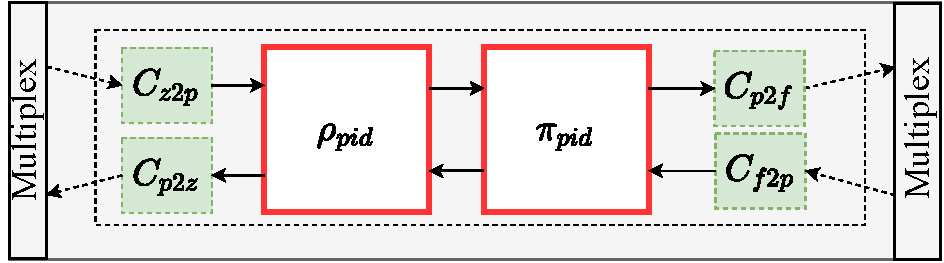
\includegraphics[scale=0.5]{figures/newcompose.pdf}
\caption{When we compose two protocols, we connect the two corresponding parties of each (with the same \m{pid}, in the way of Figure~\ref{newpandq}. The arrows between \RHO and \PI abstract away communicatior details. The communicators on the right side of \PI correspond to the type of \PI with it's hybrid \F.}
\label{fig:replacement}
\end{figure}

%The code for the operator has the same type as any other protocol except, from the description above, it's offered channel is for the type of the functionality $\F_1$ instead of $\F_2$.
%We rely on the code generation for to handle spawning instaces of a \inline{p2f} process corresponding to $\pi$ rather than $\rho$.
%The operator is given in Figure~\ref{lst:compose}.
%\begin{figure}
%\begin{lstlisting}[basicstyle=\footnotesize\BeraMonottFamily, frame=single, mathescape]
%$\tb{proc}$ compose[K][z,p]:
%  (pid: Int), (rng: [Bit]), (sid: session[1]),
%  (pid: Int), ($\$$z2p: z) |- ($\$$c: p) =
%{
%  $\$$ch <- PS.rho <- k rng sid pid $\$$z2p ;
%  $\$$c <- Ps.pi <- k rng sid pid $\$$ch 
%}
%\end{lstlisting}
%\caption{The composition operator accepts the same parameters as any other protocol party and offers the channel of type $p2f$ of the realizing protocol $\pi$. We connect $\rho$ to $\pi$ as an environment giving input to $\pi$. We do not need to include any import in our composition operator as the two protocols are guaranteed to be well-matched by the emulation definition. The operator replaces only one party (one \msf{pid}), and the \partywrapper instantiates parties that run the composed protocol.}
%\label{lst:compose}
%\end{figure}

We further require a composition operator for simulators and we briefly describe, in writing, how to connect two simulators \SIM{\rho} and \SIM{\pi} inside the construction simulator.
You can find the full simulator composition operator in the appendix.
\begin{itemize}
	\item Input from \Z is split between the two simulators
	\begin{itemize} 
		\item \inline{Z2A2P(pid, msg)} intended for parties of $\rho$ are passed to \SIM{\rho}
		\item \inline{Z2A2F(msg)} intended for $\F_1$ is passed to \SIM{\pi}.
	\end{itemize}
	\item Output from \SIM{\pi}: 
	\begin{itemize}
		\item \inline{A2F(msg)} for $\F_2$ and \inline{A2P(pid,msg)} for dummy parties of $\F_2$ are sent to \SIM{\rho} as \inline{Z2A2F(msg)}
		\item \inline{F2A2Z(msg)} is sent to \Z unaltered.
	\end{itemize}
	\item Output from \SIM{\rho}: 
	\begin{itemize}
		\item \inline{A2F(msg)} and \inline{A2P(pid,msg)} for $\F_3$ are sent out unaltered.
		\item \inline{F2A2Z(msg)} messages are sent to \SIM{\pi} as \inline{F2A(msg)} from $\F_2$.
		\item \inline{P2A2Z(pid,msg)} messages are sent to \Z unaltered.
	\end{itemize}
\end{itemize}
The simulator relies on simulators for $\F_1 \xrightarrow{\pi} \F_3$ and $\F_2 \xrightarrow{\rho} \F_3$ to satisfy simulation for Theorem~\ref{thm:singlecomp}.
It is clear that this construction adequately simulates the composed protocol. 
The type in the ideal world gurantees that both the real and ideal world adversaries get at least as much impor as any of the protocol parties. 
This ensures that the composed simulator has enough import to sandbox the two existing simulators and send import out to the ideal world parties and ideal funfctionality.
Therefore it is trivial to see that the composed simulator is well-resource-typed.

Another illustrative description of what composition proposes, logically, is shown by this series of UC executions where the $\equiv$ operator denotes equivalent UC executions that result from moving ITMs in and out of a sandbox, and $\approx$ indicates emulation:
\begin{align}
& \msf{execUC} \: \Z \, (\rho \circ \pi) \, \F_1 \, \DA \\
\equiv \; & \msf{execUC} \: (\Z \circ \rho) \, \pi \, \F_1 \, \DA \\
\approx \; & \msf{execUC} \: (\Z \circ \rho) \, \idealP \, \F_2 \, \SIM{\pi} \\
\equiv \; & \msf{execUC} \: \Z \, \rho \, \F_3 \, (\SIM{\pi} \circ \SIM{\rho})
\end{align}

%\item Inputs from \Z of \inline{Z2A2P(msg)} are passed to \SIM{\rho}, and inputs of \inline{Z2A2F(msg)} are passed to \SIM{\pi}.  
%\item \inline{P2A2Z(pid, msg)} outputs from \SIM{\rho} are forwarded to \Z unaltered.
%\item \inline{A2F(msg)} and \inline{A2P(pid, msg)} messages from \SIM{\pi} for $\F_2$ are sent to \SIM{\rho} as \inline{Z2A2F(msg)} and \inline{Z2A2P(pid, msg)}, respectively. 
%\item In the reverse direction, \inline{F2A2Z(msg)} messages from \SIM{\rho} are sent to \SIM{\pi} as \inline{F2A(msg)}, and, finally, \inline{F2A2Z(msg)} output generated by \SIM{\pi} is forwarded to \Z.
%\item \inline{A2P(pid,msg)}, \inline{A2F(msg)} messages from \SIM{\rho}, and \inline{P2A(pid,msg)} and \inline{F2A(msg)} from $\F_3$, are forwarded unaltered. 
%\end{itemize}

%We also provide a composition operator for simulators to construct a simulator for the composed protocol. We connect the simulatorsin the following way
%\begin{figure*}
%\begin{lstlisting}[basicstyle=\small\BeraMonottFamily, frame=single, mathescape]
%$\tb{proc}$ sim_compose[K][a2r,r2a][a2p,p2a][a2f,f2a]:
%  (k: Int), (rnd: [Bit]), (sid: session[1]),
%  (#z_to_a: comm[z2amsg[a2r][a2f]]), (#a_to_z: comm[a2zmsg[r2a,f2a]]),
%  (#a_to_p: comm[a2pmsg[a2r]]), (#p_to_a: comm[p2amsg[r2a]]), (#a_to_f: comm[a2fmsg[a2f]]), (#f_to_a: comm[f2amsg[f2a]])
%    |- ($\$$c: 1) =
%{
%  $\$$ch 
%\end{lstlisting}
%\end{figure*}

%\begin{figure*}
%\begin{lstlisting}[basicstyle=\small\BeraMonottFamily, frame=single,  mathescape]
%$\tb{proc}$ compose[K][z2r][r2z][f2r][r2f][p2f][f2p] : 
%    (pid: Int), ($\$$z_to_p: c[K][z2p]), ($\$$p_to_z: c[K][r2z]), 
%    ($\$$f_to_p: c[K][f2r]), ($\$$p_to_f: c[K][r2f])  |- ($\$$D : 1) =
%{
%	$\$$rho_to_pi <- $\tm{createchan}$[K][p2f];
%	$\$$pi_to_rho <- $\tm{createchan}$[K][f2p];
%
%	 <- pi  <-                 $\$$rho_to_pi $\$$pi_to_rho $\$$p_to_f $\$$f_to_p ;
%	 <- phi <- $\$$z_to_p $\$$p_to_z $\$$rho_to_pi $\$$pi_to_rho ; 
%}
%\end{lstlisting}
%\caption{Composition operator in Nomos that connects a protocol $\rho$ to a protocol $\pi$ that uses some functionality $\F$. The operators creates new channels to connect the realizing $\pi$ and it's hybrid \F. Output from $\rho$ intended for the replace functionality are actually send to parties of $\rho$, and channels outgoing from the parties to the functionality are given to $\pi$.}
%\label{lst:compose} 
%\end{figure*}

%\begin{theorem}[Composition]\label{thm:singlecomp}
%\begin{mathpar}
%\inferrule*[right=single-compose]
%{
%	\F_1 \xrightarrow{\pi} \F_2 \semi \F_2 \xrightarrow{\rho} \F_3 \\
%}
%{
%	\F_1 \xrightarrow{\rho \circ \pi} \F_3
%}
%\end{mathpar}
%
%If \textit{well-typed} $(\pi, \F_1$) realizes $\F_2$ and ($\rho$, $\F_2$) realizes some $\F_3$, then $(\rho \circ \pi, \F_2)$ is \textit{well-typed} and realizes $\F_3$ when $\circ$ is defined as in Figure~\ref{lst:compose}.
%\end{theorem}

%\begin{proof}
%The pre-condition ensures the existence of \textit{well-resource-typed} simulators $\Sim_\rho$ for $\F_2 \xrightarrow{\rho} \F_3$ and $\Sim_\pi$ for $\F_1 \xrightarrow{\pi} \F_2$, and, it is obvious that the composed protocol is also well-resource-typed.
%We construct a simulator \Sim' for the dummy adversary to show
%\[
%	\msf{execUC}\ (\rho \circ \pi)\ \F_1\ \Z\ \A \approx \msf{execUC}\ \idealP\ \F_3\ \Z\ \Sim''
%\]	
%
%The simulator $\Sim'$ relies only simulating \SIM{\pi} and \SIM{\rho}.
%Note that \SIM{\pi} can accept messages for $\pi$ or $\F_1$, simulate them, and generate input for $\F_2$. 
%Similarly, \SIM{\rho} can take inputs for $\rho$ or $\F_2$, simulate them, and generate input for $\F_3$.
%Therefore, we connect the two simulators in the natural way:
%\begin{itemize}
%\item Inputs from \Z of \inline{Z2A2P(msg)} are passed to \SIM{\rho}, and inputs of \inline{Z2A2F(msg)} are passed to \SIM{\pi}.  
%\item \inline{P2A2Z(pid, msg)} outputs from \SIM{\rho} are forwarded to \Z unaltered.
%\item \inline{A2F(msg)} and \inline{A2P(pid, msg)} messages from \SIM{\pi} for $\F_2$ are sent to \SIM{\rho} as \inline{Z2A2F(msg)} and \inline{Z2A2P(pid, msg)}, respectively. 
%\item In the reverse direction, \inline{F2A2Z(msg)} messages from \SIM{\rho} are sent to \SIM{\pi} as \inline{F2A(msg)}, and, finally, \inline{F2A2Z(msg)} output generated by \SIM{\pi} is forwarded to \Z.
%\item \inline{A2P(pid,msg)}, \inline{A2F(msg)} messages from \SIM{\rho}, and \inline{P2A(pid,msg)} and \inline{F2A(msg)} from $\F_3$, are forwarded unaltered. 
%\end{itemize}
%It is clear that \Sim' is able to emulate inputs from \Z to both parties of $\rho$ and the ideal functionalty $\F_1$.
%\Sim' performs constant over head in simulating two \emph{well-resource-typed}, and therefore it is clear that \Sim' is \emph{well-resource-typed}.
%When combined with the \emph{dummy lemma}, a well-resource-typed simulator exists for composition for any adversary \A. 
%The dummy lemma presented above ensures that a simulator for any \A can be constructed that is well-resource-typed for all wel-resource-typed \A.
%\end{proof}
%
%We give a simpler, high-level idea of the forst step of the proof proof here which can be understood visually:
%The $\equiv$ operator is a result of moving around ITMs (some from within other ITMs into the main UC execution) and $\sim$ refers to indistinguishability.
%In line (13) above, $\rho$ is moved into the execution environment with an unchanged simulator as no additional simulation is required: the simulator allows unfettered communication between parties of $\rho$ and \Z.

\subsection{Multisession}

\begin{theorem}[Composition]\label{thm:composition}
\begin{mathpar}
\inferrule*[right=compose]
{
	%(\pi, !\F_1) \sim (\idealP, F_2) \semi (\rho, !\F_2) \sim (\idealP, \F_3) \\ 
	!\F_1 \xrightarrow{\pi} \F_2 \semi !\F_2 \xrightarrow{\rho} \F_3 \\
	%\Rightarrow \exists \Sim(\A) \vdash (\rho^{!\F_2 \rightarrow (!\pi \, \circ \, \msf{squash})}, !\F_1) \sim (\idealP, \F_3)
}
{
	!\F_1 \xrightarrow{\rho \, \circ !\pi \circ \, \msf{squash}} \F_3
	%(\rho \, \circ \, !\pi \circ \msf{squash}, !\F_1) \sim (\idealP, \F_3)
}
\end{mathpar}
\end{theorem}
Full composition in the UC framework extends beyond the simpler composition in Theorem~\ref{thm:singlecomp} which only defines replacement of one functionality with a protocol that realizes it.
Instead, UC composition allows for replacement of any number of instances of a functionality with instances of the realizing protocol.
Theorem~\ref{thm:composition} illustrates the full composition theorem using our arrow notation, and highlights a theorem that we must prove before we can achieve full composition.
We rely on two sub-theorems that make use of the multisession extension: Theorem~\ref{thm:squash} and Theorem~\ref{thm:functor}.
Notice that Theorem~\ref{thm:compose} follows directly from Theorem~\ref{thm:singlecomp}, Theorem~\ref{thm:squash}, and Theorem~\ref{thm:functor}.

The multi-session extension of a protocol or functionality, specified by the $!$ operator (such as $!\rho$ or $!\F$), allows multiple instances of the protocol/functionality to be run within a sinlge ITM.
An ITM simulates the instances and multiplexes input/output to/from them much like the \partywrapper.


For the multisession extension of a fuctionality, the type is straightforward and ony acts to multiplex input/outpt based on the intended target \inline{ssid}.
\begin{center}
\parbox{0cm}{
\begin{tabbing}
$\m{{P2MS}[a,b]\{n,m\}} = \textcolor{red}{\getpot^n} \ichoice{\mb{Inp}: ssid \arrow a \tensor \echoice{$\=$\mb{Ok}: \textcolor{red}{\paypot^0} \; \m{P2MS[a,b]\{n,m\}},$ \\
\>$\mb{Out}: ssid \arrow b \tensor \textcolor{red}{\paypot^m} \; \m{P2MS[a,b]\{m,n\}}}}$
%\m{MS2P[a][b]\{n,m\}}}$ \\
%\mi{stype} \; \m{{MS2P}[a][b]\{n,m\}} = \echoice{\mb{Ok}: \textcolor{red}{\paypot^0} \; \m{P2MS[a][b]\{n,m\}}, \mb{Out}: ssid \product b \arrow \textcolor{red}{\paypot^m} \; \m{P2MS[a][b]\{n,m\}}}  
\end{tabbing}}
\end{center}
The multisession extension is mentioned in greater detail in the appendix.
%and the functional types that are sent to the wrapper surrounding it are given by
%\begin{lstlisting}[basicstyle=\small\BeraMonottFamily, mathescape]
%$\yo{type}$ p2ms[a] = P2MS of ssid ^ a ;
%$\yo{type}$ ms2p[b] = MS2P of ssid ^ b ;
%\end{lstlisting}
%It is important to note that we require a session type here instead of allowing !\F act as the functionality wrapper because, when composed it must communicate directly communicate, over a session-typed channel, to another protocol.
%Furthermore, the construction of !\F is the same as in the \Fro example: one session typed channel for all parties.
%In Figure~\ref{fig:multisession} illustrated the functionality wrapper (right) and the multisession extension (left) for \Fcom. 
%\begin{figure}
%\centering
%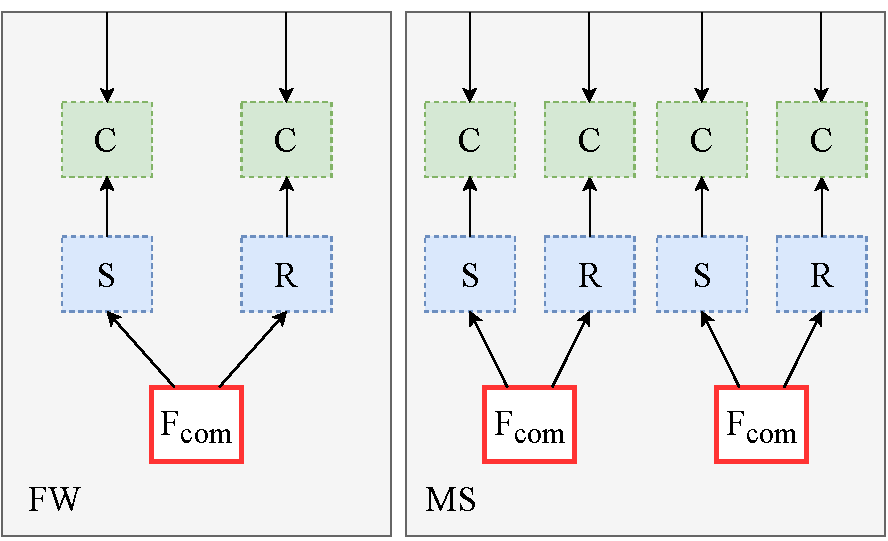
\includegraphics[scale=0.5]{figures/multisession.pdf}
%\caption{The multisession extension of \Fcom (right) with only two instances, creates the same processes $S$ and $R$ (offering the session typed channel to \Fcom) for every created instance. A communicator per session buffers messages for the $S$ and $R$ processes to consume and forward along their session-typed channel to \Fcom.}
%\label{fig:multisession}
%\end{figure}

%As a generic construction provided by NomosUC, the multisession operator requires some code generation but only to accept an arbitrary number of virtual token types if the underlying \F simulators other processes. 
%Furthermore, similar to the functionality wrapper, the multisession operator constructs the processes around \F in the same way and spawns them on-demand.
%The process definition for $!\F_\msf{com}$ is shown in Figure \ref{lst:bangf} accepting two token types: the real token type $K$ and the virtual token type $K_1$ for instances of $\F_\msf{com}$.
%
\begin{figure}
\begin{lstlisting}[basicstyle=\footnotesize\BeraMonottFamily, frame=single, mathescape]
$\tb{proc}$ bangF[K,K1][p2f,...] :
  (k: $\tgr{Int}$), (rng: [Bit]), (sid: session[a]), 
  ($\$$p: P2MS[p2f][f2p]) |- ($\$$ch: 1) =
\end{lstlisting}
\caption{The type definition for the multisession operator for functionalities and the correspond message type and import parameters. The operator for protocol parties is identical in code but differens in that the parameters to the \texttt{P2MS} type are for \texttt{Z2P} interaction.}
\label{lst:bangf}
\end{figure}

\begin{theorem}[PPT !]\label{thm:bangppt}
If a functionality $\F$ is well-resource-typed, then it's multisession extension $!\F$ is well-resource-typed.
\end{theorem}

It easy to see why the multisession extension, performing constant work and being activated a polynomial number of times, remains well-resource-typed and PPT given that \F is PPT.
We formally treat this and the remaining theorems in this section in the Appendix.

\begin{theorem}[Something About Functors]\label{thm:functor}
	\begin{mathpar}
		\inferrule*[right=somefunctor]
		{
			\F_1 \xrightarrow{\pi} \F_2
		}
		{
			!\F_1 \xrightarrow{!\pi} !\F_2
		}
	\end{mathpar}
\end{theorem}
Theorem~\ref{thm:functor} is intuitive in the sense that each session of the real world protocol $\pi$ communicates with an analogous session of $\F_1$ in isolation to realize the corresponding instance of $\F_2$. 
A UC proof for this is more involved that just providing a simulator but, instead, relies on a hybrid argument. 
We leave the bulk of the hybrid argument to Appendix~\ref{app:ms}.

\begin{theorem}[Squash Theorem]\label{thm:squash}
	\begin{mathpar}
		\inferrule*[right=squash]
		{
			\textit{well-resource-typed} \; \F
		}
		{
			!\F \xrightarrow{\msf{squash}} !!\F
		}
	\end{mathpar}
\end{theorem}
The Squash theorem, is more straightforward to prove than Theorem~\ref{thm:functor}.
It is a direct \todo{finish explaining and shove off to the Appendix.}


%\begin{proof}
%A \textit{well-resource-typed} \F guarantees a polynomial $T_{\F}$ bounding its execution.
%In the worse-case, the multisession operator must spawn a new instance of $\F$ an every activation. 
%Let $N_{\F}$ denote the total number of instances (and, hence, number of activations) of $\F$ created by the operator.
%Note that $N_{\F}$ is polynomial in the security parameter $k$ for all well-typed environments, protocols, and adversary.
%Therefore, there always exists a bounding polynomial to bound a polynomial number of simulated instances of \F.
%The polynomial can be given as:
%$$ P_{!\F}(n) = N_{\F} P_{\F}(n) + \mathcal{O}(N_{\F}) $$
%where the $\mathcal{O}(N_{\F})$ is due to the overhead of maintaining and accessing the set of all instances.
%
%Similarly, \F being \textit{well-resource-typed} ensures a valid token context for all processes it may simulate. 
%Therefore, it is clear that there exists a global connecting poltnomial $f$ that ensures a valid token context for $!\F$.
%\end{proof}


%\begin{figure}
%\begin{lstlisting}[basicstyle=\small\BeraMonottFamily, mathescape, frame=single]
%$\yo{type}$ p2bFmsg[a] = P2bF of ssid ^ a ;
%$\yo{type}$ p2bbFmsg[a] = P2bbF of ssid ^ ssid ^ a ;
%$\tg{(* z2p : comm[z2pmsg[p2bbf[a]]] *)}$
%$\tg{(* p2f : comm[p2fmsg[P2bf[a]]] *)}$
%pid = recv $\$$z2p ;
%m = recv $\$$z2p ;
%case m (
%  P2bbF(ssid1, ssid2, m) =>
%    send $\$$p2f P2bF(ssid1 + ssid2, m) ;
%)
%\end{lstlisting}
%\caption{The \textit{squash protocol} accepts a message intended intended for $!!\F$ of type \inline{P2MS[p2ms[a]][ms2p[b]]}, i.e. of the form $(\msf{ssid}_1, (\msf{ssid}_1, msg))$.
%It ``flattens'' it into a single $\msf{ssid}_3 = \msf{ssid}_1 + \msf{ssid}_2$ that can be passed to $!\F$. The result is the same number of instances of \F but behind only a single $!$ operator.}
%\label{fig:squash}
%\end{figure}

\begin{proof} (Theorem~\ref{thm:squash})
On examination the \msf{squash} theorem does constant work per activation and concantenates two \inline{ssid}s into one for messages going to the functionality and does the inverse for messages incoming from the functionality.
We provide more detail for a proof of Theorem~\ref{thm:squash} in the Appendix, however, it is clear to see that the this theorem holds with a trivial simulator.
%First we describe the \msf{squash} protocol where $!!\F$ are nested $!$ operators.
%The protocol accepts messages intended for $!!\F$ of type \inline{P2MS[p2ms[a]][ms2p[b]]}, i.e. of the form $(\msf{ssid}_1, (\msf{ssid}_2, msg))$, and ``flattens'' them into a single message of type $\inline{P2MS[a][b]}$, i.e. of the form $(\msf{ssid}_3, msg)$.
%
%In $(\idealP, !!\F)$, \idealP~expects to receive messages of the form $(\msf{ssid}_1, (\msf{ssid}_2, m))$ where $\msf{ssid_2}$ is a sub-session of $\F$ (i.e. instance) inside some $!\F$ with sub-session id $\msf{ssid}_1$ inside of $!!\F$ (the message accesses functionality $\F[\msf{ssid}_1][\msf{ssid}_2]$).
%The \msf{squash} protocol flattens the indexing of instances of \F and combines session ids $\msf{ssid}_1$ and $\msf{ssid}_2$ into a single \msf{ssid}: $\msf{ssid}_3 := \msf{ssid}_1 \cdot \msf{ssid}_2$.
%If follows intuitively that the view for the environment remains the same. 
%
%We construct a simulator such that:
%\[
%\msf{execUC} \, \Z \, \idealP \, !!\F \, \SIM{\msf{squash}} \approx \msf{execUC} \, \Z \, \msf{squash} \, !\F \DA 
%\]
%The simulator is very simple. 
%Inputs to/from parties/\Z for a corrupt party is forwarded unmodified.
%Input intended for $!\F$ of the form $(\msf{ssid}_1 \cdot \msf{ssid}_2, msg)$ is sent as $(\msf{ssid}_1, (\msf{ssid}_2, msg))$ to $!!\F$. 
%Output from $!!\F$ is modified inversely and sent to \Z.
%
%The proposed simulator is trivially analyzed to be \textit{well-resource-typed}.
%It performs constant work per activation and does ``real'' simulation other than message modification to/from $!!\F$.
\end{proof}

\subsection{UC Composition}
Finally, we can conclude with full composition in Theorem~\ref{thm:compose}.
The proof follows directly from Theorems~\ref{thm:singlecomp} and \ref{thm:squash}.

\begin{proof}
By Theorem~\ref{thm:singlecomp} we can construct a simulator \SIM{1} for $!!\F_1 \xrightarrow{\rho \, \circ \, !\pi} \F_3$.
Theorem~\ref{thm:squash} then allows us to ``squash'' $!!\F_1$ and construct a simulator using \SIM{1} for $!\F_1 \xrightarrow{\rho \, \circ \, !\pi \, \circ \, \msf{squash}} \F_3$
\end{proof}


